% Options for packages loaded elsewhere
% Options for packages loaded elsewhere
\PassOptionsToPackage{unicode}{hyperref}
\PassOptionsToPackage{hyphens}{url}
\PassOptionsToPackage{dvipsnames,svgnames,x11names}{xcolor}
%
\documentclass[
  titlepage]{article}
\usepackage{xcolor}
\usepackage{amsmath,amssymb}
\setcounter{secnumdepth}{5}
\usepackage{iftex}
\ifPDFTeX
  \usepackage[T1]{fontenc}
  \usepackage[utf8]{inputenc}
  \usepackage{textcomp} % provide euro and other symbols
\else % if luatex or xetex
  \usepackage{unicode-math} % this also loads fontspec
  \defaultfontfeatures{Scale=MatchLowercase}
  \defaultfontfeatures[\rmfamily]{Ligatures=TeX,Scale=1}
\fi
\usepackage{lmodern}
\ifPDFTeX\else
  % xetex/luatex font selection
\fi
% Use upquote if available, for straight quotes in verbatim environments
\IfFileExists{upquote.sty}{\usepackage{upquote}}{}
\IfFileExists{microtype.sty}{% use microtype if available
  \usepackage[]{microtype}
  \UseMicrotypeSet[protrusion]{basicmath} % disable protrusion for tt fonts
}{}
\makeatletter
\@ifundefined{KOMAClassName}{% if non-KOMA class
  \IfFileExists{parskip.sty}{%
    \usepackage{parskip}
  }{% else
    \setlength{\parindent}{0pt}
    \setlength{\parskip}{6pt plus 2pt minus 1pt}}
}{% if KOMA class
  \KOMAoptions{parskip=half}}
\makeatother
% Make \paragraph and \subparagraph free-standing
\makeatletter
\ifx\paragraph\undefined\else
  \let\oldparagraph\paragraph
  \renewcommand{\paragraph}{
    \@ifstar
      \xxxParagraphStar
      \xxxParagraphNoStar
  }
  \newcommand{\xxxParagraphStar}[1]{\oldparagraph*{#1}\mbox{}}
  \newcommand{\xxxParagraphNoStar}[1]{\oldparagraph{#1}\mbox{}}
\fi
\ifx\subparagraph\undefined\else
  \let\oldsubparagraph\subparagraph
  \renewcommand{\subparagraph}{
    \@ifstar
      \xxxSubParagraphStar
      \xxxSubParagraphNoStar
  }
  \newcommand{\xxxSubParagraphStar}[1]{\oldsubparagraph*{#1}\mbox{}}
  \newcommand{\xxxSubParagraphNoStar}[1]{\oldsubparagraph{#1}\mbox{}}
\fi
\makeatother


\usepackage{longtable,booktabs,array}
\usepackage{calc} % for calculating minipage widths
% Correct order of tables after \paragraph or \subparagraph
\usepackage{etoolbox}
\makeatletter
\patchcmd\longtable{\par}{\if@noskipsec\mbox{}\fi\par}{}{}
\makeatother
% Allow footnotes in longtable head/foot
\IfFileExists{footnotehyper.sty}{\usepackage{footnotehyper}}{\usepackage{footnote}}
\makesavenoteenv{longtable}
\usepackage{graphicx}
\makeatletter
\newsavebox\pandoc@box
\newcommand*\pandocbounded[1]{% scales image to fit in text height/width
  \sbox\pandoc@box{#1}%
  \Gscale@div\@tempa{\textheight}{\dimexpr\ht\pandoc@box+\dp\pandoc@box\relax}%
  \Gscale@div\@tempb{\linewidth}{\wd\pandoc@box}%
  \ifdim\@tempb\p@<\@tempa\p@\let\@tempa\@tempb\fi% select the smaller of both
  \ifdim\@tempa\p@<\p@\scalebox{\@tempa}{\usebox\pandoc@box}%
  \else\usebox{\pandoc@box}%
  \fi%
}
% Set default figure placement to htbp
\def\fps@figure{htbp}
\makeatother


% definitions for citeproc citations
\NewDocumentCommand\citeproctext{}{}
\NewDocumentCommand\citeproc{mm}{%
  \begingroup\def\citeproctext{#2}\cite{#1}\endgroup}
\makeatletter
 % allow citations to break across lines
 \let\@cite@ofmt\@firstofone
 % avoid brackets around text for \cite:
 \def\@biblabel#1{}
 \def\@cite#1#2{{#1\if@tempswa , #2\fi}}
\makeatother
\newlength{\cslhangindent}
\setlength{\cslhangindent}{1.5em}
\newlength{\csllabelwidth}
\setlength{\csllabelwidth}{3em}
\newenvironment{CSLReferences}[2] % #1 hanging-indent, #2 entry-spacing
 {\begin{list}{}{%
  \setlength{\itemindent}{0pt}
  \setlength{\leftmargin}{0pt}
  \setlength{\parsep}{0pt}
  % turn on hanging indent if param 1 is 1
  \ifodd #1
   \setlength{\leftmargin}{\cslhangindent}
   \setlength{\itemindent}{-1\cslhangindent}
  \fi
  % set entry spacing
  \setlength{\itemsep}{#2\baselineskip}}}
 {\end{list}}
\usepackage{calc}
\newcommand{\CSLBlock}[1]{\hfill\break\parbox[t]{\linewidth}{\strut\ignorespaces#1\strut}}
\newcommand{\CSLLeftMargin}[1]{\parbox[t]{\csllabelwidth}{\strut#1\strut}}
\newcommand{\CSLRightInline}[1]{\parbox[t]{\linewidth - \csllabelwidth}{\strut#1\strut}}
\newcommand{\CSLIndent}[1]{\hspace{\cslhangindent}#1}



\setlength{\emergencystretch}{3em} % prevent overfull lines

\providecommand{\tightlist}{%
  \setlength{\itemsep}{0pt}\setlength{\parskip}{0pt}}



 


\usepackage{fvextra}
\DefineVerbatimEnvironment{Highlighting}{Verbatim}{breaklines,commandchars=\\\{\}}
\DefineVerbatimEnvironment{OutputCode}{Verbatim}{breaklines,commandchars=\\\{\}}
\makeatletter
\@ifpackageloaded{caption}{}{\usepackage{caption}}
\AtBeginDocument{%
\ifdefined\contentsname
  \renewcommand*\contentsname{Table of contents}
\else
  \newcommand\contentsname{Table of contents}
\fi
\ifdefined\listfigurename
  \renewcommand*\listfigurename{List of Figures}
\else
  \newcommand\listfigurename{List of Figures}
\fi
\ifdefined\listtablename
  \renewcommand*\listtablename{List of Tables}
\else
  \newcommand\listtablename{List of Tables}
\fi
\ifdefined\figurename
  \renewcommand*\figurename{Figure}
\else
  \newcommand\figurename{Figure}
\fi
\ifdefined\tablename
  \renewcommand*\tablename{Table}
\else
  \newcommand\tablename{Table}
\fi
}
\@ifpackageloaded{float}{}{\usepackage{float}}
\floatstyle{ruled}
\@ifundefined{c@chapter}{\newfloat{codelisting}{h}{lop}}{\newfloat{codelisting}{h}{lop}[chapter]}
\floatname{codelisting}{Listing}
\newcommand*\listoflistings{\listof{codelisting}{List of Listings}}
\makeatother
\makeatletter
\makeatother
\makeatletter
\@ifpackageloaded{caption}{}{\usepackage{caption}}
\@ifpackageloaded{subcaption}{}{\usepackage{subcaption}}
\makeatother
\usepackage{bookmark}
\IfFileExists{xurl.sty}{\usepackage{xurl}}{} % add URL line breaks if available
\urlstyle{same}
\hypersetup{
  pdftitle={Chinese Language Web Classification Model Capstone Project Report},
  pdfauthor={Mingjia ``Jacky'' Guan},
  colorlinks=true,
  linkcolor={blue},
  filecolor={Maroon},
  citecolor={Blue},
  urlcolor={Blue},
  pdfcreator={LaTeX via pandoc}}


\title{Chinese Language Web Classification Model Capstone Project
Report}
\author{Mingjia ``Jacky'' Guan}
\date{2025-08-21}
\begin{document}
\maketitle

\renewcommand*\contentsname{Table of contents}
{
\hypersetup{linkcolor=}
\setcounter{tocdepth}{3}
\tableofcontents
}
\listoffigures
\listoftables

\newpage

\section*{Abstract}\label{abstract}
\addcontentsline{toc}{section}{Abstract}

Digital technology integration in education has created significant
challenges for content filtering, particularly in non-English
educational environments where existing filtering technologies
demonstrate limited effectiveness. This study presents the development
of an enhanced Chinese Web Classification Model (CWCM) designed to
address critical limitations in current web filtering systems used
within the global K-12 education sector by constructing a comprehensive
dataset of 400k+ Chinese web content samples with focused enhancement of
three critical harmful categories: drugs, tobacco, and weapons. Using
Jieba-based text segmentation and custom TF-IDF vectorization with
strategically extracted feature dictionaries, we evaluated over 34
machine learning algorithms through rigorous 10-fold cross-validation,
with methodology incorporating statistical significance testing and
correlation analysis to examine the relationship between dataset size
and model performance across content categories. The optimized Logistic
Regression model achieved a macro-averaged F1-score of 0.9183,
demonstrating statistically significant superior performance compared to
baseline models including XGBoost (\(p < 0.000001\)) and LinearSVC
(\(p < 0.000001\)), while statistical analysis revealed strong positive
correlations between dataset size and performance metrics
(\(\rho = 0.6868\) for F1-score, \(p = 0.009\)), providing empirical
evidence for strategic data collection priorities. The model
successfully addresses deployment constraints through client-side
JavaScript implementation, enabling real-time inference on
resource-limited devices while maintaining privacy and eliminating API
dependencies, thus contributing to educational technology by providing
an effective, deployable solution for Chinese content filtering that
balances accuracy, computational efficiency, and practical
implementation requirements for protecting digital learning
environments.

\textbf{Keywords:} web content classification, Chinese natural language
processing, educational technology, machine learning, content filtering,
digital safety

\newpage

\section*{Acknowledgments}\label{acknowledgments}
\addcontentsline{toc}{section}{Acknowledgments}

I would like to thank Prof.~Zheng Qu and Prof.~Miao Yu for guidance,
Mr.~A. Y. and Mr.~B. L. for continued support and providing directions,
DLD Technologies Inc.~and Mr.~Shuang Ji for bare metal services and the
opportunity, and collaborators who provided vital feedback, without all
of whom this project would not be possible.

\section{Introduction}\label{introduction}

Digital connectivity now reaches more than half of the world's
lower-secondary classrooms, yet the very screens intended to expand
learning often become the prime source of distraction for students
(UNESCO, 2023). The next generation is now constantly immersed in
technology, with the average student-to-computer steadily rising from
7:1 in 2012 to about 3:2 in 2022 across 38 countries (OECD, 2023).
Educational departments worldwide have also been eager to adapt
technology, with over 85\% of OECD countries adopting or promoting
explicit strategies to digitize their classrooms. This effort was only
compounded by the COVID-19 pandemic, leading to over 1 billion students
worldwide adopting digital learning methods (UNESCO, 2023). With the
gradual paradigm shift--as evident by 85\% of countries having plans to
increase connectivity in the education sector--the digital age has
redefined the modern educational framework, propelling digital learning
into the mainstream (Qureshi \& Khan, 2023).

Over the past decade, investors, governments, and the education sector
have all shown great interest and confidence in education technology (ed
tech). For instance, the global market for ed tech is expected to reach
\$404 billion in 2025 (HolonIQ, 2025). There has also been a 21.5\%
year-on-year increase in related research from 2014-2023 regarding
digital education ({``Digital Education Research Trends 2014-2023,''}
2025). While there is strong enthusiasm to digitize our classrooms,
inadequate implementations of technology in education can negatively
impact student achievement, mental wellbeing, and cognitive performance.

There is substantial evidence showing that high levels of media
multitasking in an education setting--defined as simultaneously engaging
in classwork and digital media--resulted in lower overall grades and
increased distractibility (Ragan et al., 2014). Students often feel
compelled to simultaneously juggle academic materials, social media
notifications, as well as audio-visual content when presented with
technology in an academic setting. Laboratory and field experiments
demonstrate that task-switching to unrelated digital content overloads
cognitive resources, resulting in diminished comprehension, memory
retention, and critical thinking during learning tasks, also known as
``brain drain.'' (Levine et al., 2012; Ward et al., 2017)

The decline in attention span is strongly linked to the presence and
increasing influence of digital technology, both inside and outside the
classroom. According to a 2024 study conducted by the Programme for
International Student Assessment (PISA), nearly one in three students
(30\%) across OECD countries reported being distracted by digital
devices in ``most or every'' math lesson (OECD, 2024). In countries such
as Argentina, Uruguay, and Chile, over 50\% of students have reported a
high frequency of digital distraction in a classroom setting (OECD,
2024). A study published by the Institute for Labor Economics in April
2018 already found that 80\% of students engage with two electronic
devices simultaneously while studying (\emph{Student Device Usage
Patterns}, 2018).

Further research suggest that the negative impact of unrestricted and
ubiquitous media use does not limit itself to K-12 or even the education
system. For instance, a 2014 study shows that students with laptops in
universities engage in content unrelated to the task at hand for roughly
two-thirds of the time (Junco, 2014). In our daily lives, multimedia
exposure has led to a significant change in attention span, increased
distractability, and heightened impulsivity ({``Task Switching and
Cognitive Performance,''} 2013). Given the expansion of multimedia
device use, these phenomena and figures are likely to be higher today.
Most of these studies do not point to technology being the issue --
rather, it is the distraction factor that comes with technology, a
factor children have a difficult time reducing by themselves. One often
finds existing studies focusing on digital prevalence and outcomes
thereof, with less attention to how novel technological interventions
could mitigate distraction and underperformance.

\subsection{The Loopholes of Legacy
Technology}\label{the-loopholes-of-legacy-technology}

As a direct result of this international trend to digitize education,
the ed tech sector should have improved the development of resources
that are effective at filtering the internet for appropriate use in
classrooms. Legacy web filtering technologies typically operate through
one of three primary mechanisms: Uniform Resource Locator (URL)
filtering, Domain Name System (DNS) filtering, or proxy-based filtering.
URL filtering works by comparing requested web addresses against
predetermined block-or-allow lists. DNS filtering intervenes during the
domain name resolution process, blocking or allowing connections from
entire domains before content is accessed. Proxy-based filtering routes
traffic through intermediary servers that inspect and filter requests
based on predefined rules.

While these approaches offer advantages such as operational speed,
reduced processing overhead, and high scalability when implemented with
comprehensive blocklists, they suffer from significant technical
limitations. The most notable constraint is their limited granularity,
typically operating at the URL/domain level rather than analyzing
specific content on individual webpages. This binary approach to access
control (either allowing or blocking entire domains) creates particular
challenges in educational environments where nuanced content
distinctions are essential. For instance, a traditional filter might
block or allow an entire news website, without distinguishing between
educational news articles, inappropriate content, or entertainment
sections on the same domain. Similarly, video streaming platforms
contain both valuable educational content and material unsuitable for
classroom settings, yet traditional filters lack the capability to
differentiate between these content types within the same platform.

Legacy filtering technologies are also vulnerable to various
circumvention techniques. Students with basic networking knowledge are
able to use public DNS servers to bypass such implementations by IT
administrators. Virtual Private Networks (VPNs) provide another evasion
route by encrypting traffic and routing it through external servers.
Another common method is through web-proxies, where students access
websites through intermediary servers that fetch content on behalf of
the student-operated device, thus avoiding direct connections, which
would potentially flag inappropriate use. Additionally, specialized
circumvention websites and browser extensions continuously emerge,
designed specifically to bypass school filtering systems. Even if a
combination of such technologies is used, it is still difficult for
schools to effectively manage technology access within their network.

However, the educational-technological landscape is perhaps one of the
most dynamic markets in today's economy, with complete product updates
happening every 36 months on average (UNESCO, 2023). In response to
these limitations, next-generation filtering technologies have emerged
that provide more sophisticated content analysis capabilities. Unlike
traditional methods that simply block entire domains, content-aware
filtering systems analyze the actual content of web pages, including
text, images, and videos in real time. This ensures that there is little
to no delay between the harmful content appearing on the device and a
filter blocking it. This approach is particularly valuable in
educational settings where new harmful content can emerge rapidly, and
traditional methods become ineffective or obsolete in the ed tech
landscape.

\subsection{Integrating Machine
Learning}\label{integrating-machine-learning}

The integration of artificial intelligence and machine learning has
revolutionized web filtering capabilities, enabling systems to recognize
patterns, learn from new threats, and make increasingly accurate content
classifications without relying solely on predetermined rules. One
enhancement that could be made to legacy technology is to intercept the
network request traffic at the DNS resolution step before into a
pre-trained machine learning (ML) model to determine whether to allow or
deny access to the requested site (Jare \& Kolte, 2023). The present
study investigates the development of a client-level interceptor
application capable of real-time parsing and analysis of website source
code through the application of pre-trained machine learning algorithms.
This algorithm will be able to separate websites into several
pre-determined categories, leaving it up to the individual school
administrator to block or unblock, not based on granular websites, but
rather on refined categories. As a result, our ML-based web filter will
keep students on track and instantly prohibit technological
distractions, offering real-time results when delivering results and
providing a significant improvement in performance over legacy filtering
technology.

\section{Background and Related Work}\label{background-and-related-work}

The landscape of machine learning and natural language processing has
undergone a remarkable transformation over the past decade, evolving
from traditional statistical methods to sophisticated deep learning
architectures capable of understanding complex linguistic patterns and
contextual relationships. Earlier generation models, particularly
sequence-to-sequence architectures, struggled with fundamental
limitations in contextual understanding, often failing to capture
long-range dependencies and nuanced semantic relationships within text.
The introduction of the attention mechanism, popularized by the seminal
``Attention is All You Need'' paper, marked a pivotal breakthrough by
enabling models to dynamically focus on relevant parts of input
sequences when generating output tokens, effectively learning the
relevance and relationships between words without explicit supervision
through the use of additional context vectors. This fundamental shift
toward attention-based architectures not only revolutionized natural
language processing but also laid the groundwork for the
transformer-based models that dominate today's AI landscape. To
understand this evolution fully, it is essential to examine both the
traditional machine learning approaches that preceded these
advances---including boosted trees and support vector machines---as well
as the progression of deep learning architectures from recurrent neural
networks through to modern transformer-based models like BERT and its
variants.

\subsection{Logistic Regression}\label{logistic-regression}

Logistic regression transforms linear combinations of features into
probabilities using the sigmoid function, an S-shaped curve that maps
any real number to a value between 0 and 1. Unlike linear regression,
this approach directly models probabilities, ensuring outputs remain
within valid ranges. The model finds optimal parameters through Maximum
Likelihood Estimation (MLE), which maximizes the likelihood of observing
the training data. The resulting cost function (cross-entropy loss) is
convex, guaranteeing that optimization algorithms find the global
optimum rather than getting stuck in local minima.

For multi-class problems, two main approaches exist: One-vs-Rest creates
separate binary classifiers for each class, while multinomial logistic
regression directly models probabilities across all classes using the
softmax function. Multinomial approaches generally provide better
calibrated probabilities ({``Better Calibrated Probabilities in Machine
Learning Models,''} 2024). High-dimensional datasets with thousands of
features face the curse of dimensionality, where data becomes sparse and
overfitting increases. Three regularization techniques address this: L1
(Lasso) drives coefficients to zero for automatic feature selection, L2
(Ridge) shrinks coefficients while maintaining numerical stability, and
Elastic Net combines both approaches to balance feature selection with
grouping of correlated features.

Scikit-learn's LogisticRegression class effectively handles
high-dimensional sparse data through key parameters: the penalty type,
the SAGA solver (best for scalability and all penalty types),
regularization strength C (typically starting at 1.0 and inversely
proportional to the strength of the regularization), and increased
maximum iterations (1,000-10,000 for convergence).

\subsection{Boosted Trees}\label{boosted-trees}

During the initial model selection round, XGBoost was selected as a
representative of the boosted trees family of classifiers. Boosted trees
are ensemble machine learning models, sequentially fitting trees in a
forward, stagewise fashion, where each new tree is trained to correct
the errors made by the previous trees ({``A Working Guide to Boosted
Regression Trees,''} 2008). This creates an additive model where
individual terms are simple trees that together form a powerful
predictor.

Boosted trees overcome the biggest drawback of single tree models -
their inability to generalize to larger distributions of data. While
maintaining the strengths of tree-based methods (handling different
variable types, accommodating missing data, and fitting complex
nonlinear relationships), boosted trees achieve much higher predictive
performance compared to single trees, often surpassing most traditional
modeling methods in terms of out-of-box performance. They're
particularly dominant for tabular data tasks and can achieve both
accurate prediction and meaningful explanation simultaneously, making
them one of the most successful traditional machine learning approaches
available.

At each iteration during the training process for boosted training
algorithms, new trees are trained on pseudo-residuals (negative
gradients of the loss function), effectively moving the ensemble toward
optimal predictions through sequential learning. Most modern boosting
frameworks enhance basic gradient boosting through various optimization
techniques including second-order derivatives, regularization terms, and
sophisticated tree-building strategies. The regularization components
prevent overfitting through tree structure constraints (controlling tree
depth, minimum leaf weights, and split requirements) and weight
penalties using L1 and L2 regularization methods.

For multiclass classification, boosting frameworks typically employ
softmax objectives where class probabilities are computed using
exponential functions normalized across all classes, optimizing
multiclass log-loss across all classes simultaneously. Different
frameworks implement multiclass classification through various
strategies including one-vs-rest, one-vs-one, or direct multiclass
approaches. When handling high-dimensional sparse data, modern boosting
frameworks leverage compressed storage formats for memory efficiency,
sparse-aware algorithms that handle missing values intelligently, and
feature subsampling strategies at multiple granularities to achieve
significant computational savings while maintaining performance.

Hyperparameter tuning across boosting frameworks generally follows
hierarchical approaches: first optimizing core tree parameters (maximum
depth, minimum samples), then regularization parameters (weight
penalties, subsampling ratios), and finally efficiency parameters
specific to each implementation. The learning rate controls how much
each weak learner contributes to the final ensemble, where lower
learning rates require more iterations but generally produce better
generalization. The optimal number of boosting rounds is typically
inversely related to the learning rate, with frameworks balancing
training speed and generalization through regularization and early
stopping mechanisms.

\subsubsection{LightGBM}\label{lightgbm}

LightGBM is a gradient boosting framework that achieves high speed and
memory efficiency via histogram-based split finding, leaf-wise
(best-first) tree growth, and two core innovations: Gradient-based
One-Side Sampling (GOSS) to prioritize high-gradient instances and
Exclusive Feature Bundling (EFB) to compress sparse, mutually exclusive
features ({``LightGBM,''} 2017). These design choices typically yield
faster training than conventional level-wise boosters at comparable
accuracy, with strong scalability and distributed/GPU support reported
across applications. Key weaknesses include sensitivity to
hyperparameters due to leaf-wise growth, which can overfit without
depth/leaf constraints; practical tuning difficulty; and potential
memory intensity on very large, high-dimensional data despite overall
efficiency gains.

\subsubsection{XGBoost}\label{xgboost}

XGBoost is a regularized gradient boosting implementation known for
robust accuracy on tabular data, with features such as L1/L2
regularization much like LightGBM, but also sparsity-aware split finding
that learns default directions for missing values, and approximate split
methods such as weighted quantile sketch to scale training (Chen \&
Guestrin, 2016). Like LightGBM, models still require careful tuning and
can overfit if regularization and early stopping are not used
appropriately. Limitations often cited are heavier computational and
memory costs relative to newer histogram/leaf-wise designs and a
comparatively steeper configuration burden to reach peak performance on
large datasets.

\subsection{LinearSVC}\label{linearsvc}

Support Vector Machines represent one of the most theoretically grounded
and practically effective machine learning algorithms, particularly
well-suited for high-dimensional sparse data classification tasks. The
mathematical elegance of SVMs stems from their foundation in statistical
learning theory and convex optimization, making them especially powerful
for datasets with thousands of features where traditional methods often
struggle. Unlike many algorithms that suffer from the curse of
dimensionality, SVMs often improve performance as dimensionality
increases, making them ideal candidates for modern data science
challenges involving feature-rich yet extremely sparse datasets
({``Support Vector Machines as Ideal Candidates for Sparse Data
Classification,''} 2018; {``Support Vector Machines Performance in High
Dimensional Data,''} 2017).

The core strength of linear SVMs lies in their ability to find optimal
decision boundaries through a process that balances margin maximization
with empirical risk minimization. This optimization problem seeks to
identify the hyperplane that best separates different classes with
modest error tolerance with slack variables. The resulting model depends
only on a subset of training points called support vectors, which
provides both computational efficiency (with the exploitation of the
kernel trick) and strong generalization capabilities (Wen, 2018). This
sparse representation is particularly advantageous when working with
high-dimensional data, as the model complexity depends on the number of
support vectors rather than the total dimensionality of the feature
space.

For high-dimensional sparse data applications, particularly those
involving thousands of features, scikit-learn's LinearSVC implementation
provides significant computational advantages over general SVM
approaches, as it utilizes the LIBLINEAR library under the hood
(developers, n.d.; Fan et al., 2008). The algorithm leverages coordinate
descent optimization that scales linearly with both samples and
features, enabling training on datasets with hundreds of thousands of
examples in seconds rather than hours required by general SVM solvers.
Additionally, LIBLINEAR's support for both L1 and L2 regularization
enables automatic feature selection and model regularization,
effectively identifying the most relevant predictors while maintaining
computational efficiency.

This combination of exceptional speed, theoretical foundation, and
practical accessibility makes LinearSVC an excellent choice for
classification tasks in high-dimensional sparse environments where
traditional nonlinear SVM methods may be computationally prohibitive.

\subsection{Modern Deep Learning
Algorithms}\label{modern-deep-learning-algorithms}

The evolution from traditional machine learning approaches to modern
deep learning represents a fundamental shift in how machines process and
understand language. While boosted trees and linear SVMs excel with
structured tabular data, the complexity of natural language
understanding demanded more sophisticated architectures capable of
capturing contextual relationships and semantic meaning at scale.

\subsubsection{Recurrent Neural Networks and Sequential
Processing}\label{recurrent-neural-networks-and-sequential-processing}

The foundation of modern NLP began with Recurrent Neural Networks
(RNNs), which introduced the revolutionary concept of sequential
information processing (Jordan, 1986; Schmidt, 2019). Unlike feedforward
networks that process inputs independently, RNNs maintain hidden states
that carry information across time steps, enabling them to understand
context within sequences. The mathematical formulation shows this
clearly:

\[
H_t = \phi_h X_t W_{xh} + H_{t-1} W_{hh} + b_h
\]

However, vanilla RNNs suffered from the vanishing gradient problem,
where information from distant past tokens would effectively disappear
during backpropagation through time This limitation was partially
addressed by Long Short-Term Memory (LSTM) units, which introduced
gating mechanisms to selectively retain and forget information across
longer sequences.

\subsection{Long Short-Term Memory (LSTM) Networks: Solving the Memory
Problem}\label{long-short-term-memory-lstm-networks-solving-the-memory-problem}

While vanilla RNNs introduced the groundbreaking concept of sequential
processing, they suffered from a fundamental limitation that severely
restricted their practical applications: the vanishing gradient problem.
As information propagated backward through time during training, error
signals would exponentially decay, making it nearly impossible for
networks to learn dependencies spanning more than a few time steps. The
mathematical foundation shows that gradients scale by products of weight
matrices and activation function derivatives across time steps, causing
exponential decay when values are consistently less than 1.0 or
explosive growth when greater than 1.0.

\begin{figure}[H]

{\centering \pandocbounded{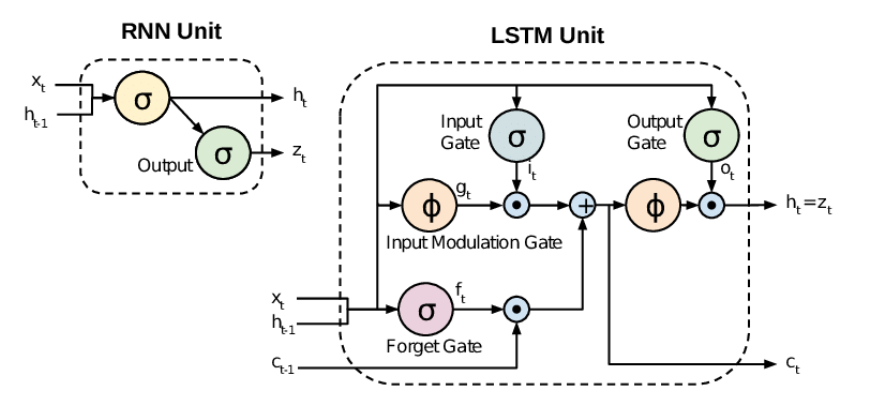
\includegraphics[keepaspectratio]{figures/rnn-vs-lstm.png}}

}

\caption{RNN vs LSTM comparison diagram (Tripathi, 2021)}

\end{figure}%

Long Short-Term Memory (LSTM) networks, introduced by Hochreiter and
Schmidhuber in 1997, revolutionized sequential modeling by introducing
sophisticated gating mechanisms that enable constant error flow through
specially designed memory cells (Hochreiter \& Schmidhuber, 1997). The
LSTM architecture centers around memory cells with linear
self-connections called ``Constant Error Carousels'' (CECs), protected
by three types of gates: input gates that control when new information
should be stored, forget gates that decide what information should be
discarded, and output gates that control when stored information should
influence other units. The genius of LSTM lies in these multiplicative
gates, which solve the conflicting weight update problem by providing
context-sensitive control mechanisms---the input gate learns when to
write to memory, the forget gate learns what to discard, and the output
gate learns when to read from memory, all while the memory cell
maintains constant error flow through its linear self-connection.

LSTM's ability to bridge time intervals exceeding 1000 steps
fundamentally changed what was possible in language modeling and
sequential tasks. Unlike previous approaches that could only capture
short-term dependencies, LSTMs could maintain coherent representations
of linguistic context across entire paragraphs or documents, enabling
practical applications in machine translation, where source sentence
information needed to be preserved while generating target translations,
and in language modeling, where long-range syntactic and semantic
dependencies could finally be captured effectively. LSTM variants and
improvements continued to dominate sequence modeling until the
transformer revolution, with architectures like GRUs (Gated Recurrent
Units) simplifying the gating mechanism while maintaining the core
benefits of selective memory management.

The real breakthrough came with bidirectional processing capabilities,
where models could consider both past and future context simultaneously.
This bidirectional approach proved crucial for tasks requiring
comprehensive understanding of linguistic context, laying the groundwork
for the LSTM and subsequent transformer revolution that followed.

\subsubsection{The Transformer Architecture
Revolution}\label{the-transformer-architecture-revolution}

The seminal ``Attention is All You Need'' paper fundamentally changed
the landscape by introducing the Transformer architecture, abandoning
recurrence entirely in favor of self-attention mechanisms (Vaswani et
al., 2017). This paradigm shift enabled models to attend to all
positions in a sequence simultaneously, dramatically improving both
training efficiency and the model's ability to capture long-range
dependencies.

The attention mechanism allows the model to dynamically focus on
relevant parts of the input when processing each token, similar to how
humans selectively attend to different words when comprehending text.
Multi-head attention extends this capability by allowing the model to
attend to information from different representation subspaces
simultaneously, creating a rich understanding of contextual
relationships.

\subsubsection{BERT and Bidirectional Language
Understanding}\label{bert-and-bidirectional-language-understanding}

\begin{figure}[H]

{\centering \pandocbounded{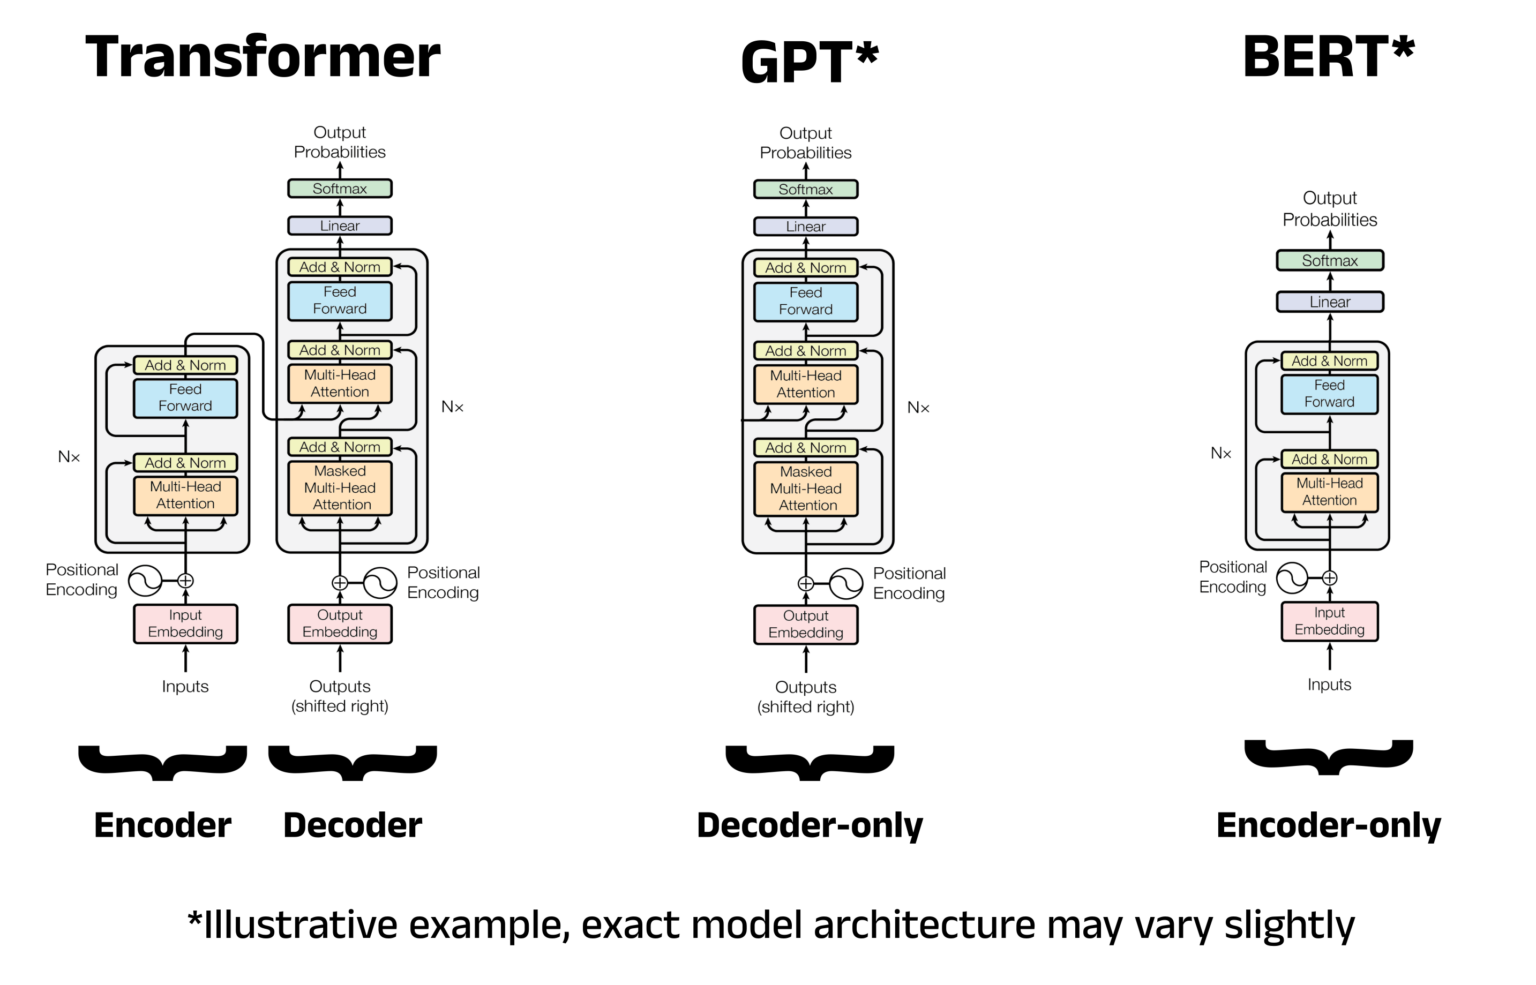
\includegraphics[keepaspectratio]{figures/transformer_architecture.png}}

}

\caption{A comparison of the architectures for the Transformer, GPT, and
BERT (Smith, 2024)}

\end{figure}%

BERT (Bidirectional Encoder Representations from Transformers)
represented a revolutionary paradigm shift in natural language
processing by introducing truly bidirectional pre-training through its
innovative masked language modeling approach (Devlin et al., 2018).
Unlike its predecessors, such as GPT and ELMo, which processed text in a
unidirectional manner or used shallow concatenation of independently
trained left-to-right and right-to-left models, BERT's architecture
enables the model to condition on both left and right context
simultaneously across all layers of the network (Peters et al., 2018;
Radford et al., 2018).

The fundamental innovation lies in BERT's use of the Transformer encoder
architecture with bidirectional self-attention. In traditional
left-to-right language models, each token can only attend to previous
tokens in the self-attention layers, creating a fundamental limitation
in understanding context. BERT overcomes this constraint by employing a
``masked language model'' (MLM) pre-training objective inspired by the
Cloze task. During training, the model randomly masks 15\% of the input
tokens and attempts to predict these masked tokens based on the complete
bidirectional context. This approach forces the model to learn rich
representations that incorporate information from both directions of the
sequence.

The masking strategy itself is carefully designed to prevent the model
from simply memorizing token positions. When a token is selected for
masking, 80\% of the time it is replaced with the special {[}MASK{]}
token, 10\% of the time it is replaced with a random token from the
vocabulary, and 10\% of the time it remains unchanged. This stochastic
approach ensures that the model learns to predict tokens based on
contextual understanding rather than positional cues, while also
addressing the mismatch between pre-training (where {[}MASK{]} tokens
appear) and fine-tuning (where they do not).

The second pre-training objective, Next Sentence Prediction (NSP), was
designed to help the model understand relationships between sentence
pairs, which is crucial for downstream tasks like question answering and
natural language inference. During pre-training, the model receives
pairs of sentences where 50\% are consecutive sentences from the same
document (labeled as ``IsNext'') and 50\% are random sentence pairs from
different documents (labeled as ``NotNext''). This objective enables
BERT to learn discourse-level representations that capture
inter-sentence relationships.

The architectural foundation of BERT relies heavily on the Transformer's
multi-head self-attention mechanism, which allows each token to attend
to all other tokens in the sequence simultaneously. This bidirectional
attention enables the model to build rich contextual representations
where each token's representation is influenced by the entire sequence
context. The model processes input through multiple layers of
self-attention and feed-forward networks, with each layer refining the
representations by incorporating increasingly complex linguistic
patterns and relationships.

BERT's input representation is particularly sophisticated, combining
token embeddings, segment embeddings, and positional embeddings. Token
embeddings represent the actual words or subwords, segment embeddings
distinguish between different sentences in a pair, and positional
embeddings provide sequence order information. This multi-faceted
representation allows the model to understand not just what tokens
appear in the sequence, but also their roles and relationships within
the broader context.

The impact of this bidirectional approach was immediately apparent in
BERT's performance across a wide range of NLP tasks. The model achieved
new state-of-the-art results on eleven different tasks, including a
remarkable 7.7\% absolute improvement on the GLUE benchmark (Wang et
al., 2018). This success demonstrated that bidirectional pre-training
could capture linguistic phenomena that were previously difficult for
unidirectional models to learn, such as syntactic dependencies that span
long distances and semantic relationships that require understanding of
both preceding and following context.

\subsection{Optimization and Scaling
Improvements}\label{optimization-and-scaling-improvements}

RoBERTa (Robustly Optimized BERT Pretraining Approach) emerged as a
systematic investigation into the training procedures and
hyperparameters that contribute to BERT's success, revealing that many
of the performance gains attributed to architectural innovations were
actually due to suboptimal training configurations in the original BERT
implementation (Liu et al., 2019). The research demonstrated that BERT
was significantly undertrained and that careful optimization of the
training process could yield substantial improvements without any
architectural modifications.

One of the most significant findings was the impact of training duration
and batch size scaling. While the original BERT was trained for 1
million steps with a batch size of 256 sequences, RoBERTa experiments
showed that training with larger batches (up to 8,000 sequences) for
extended periods dramatically improved performance. The research
revealed that training with large batches not only improved optimization
speed but also enhanced end-task performance when the learning rate was
appropriately adjusted. This finding challenged conventional wisdom
about batch size limitations and demonstrated that modern optimization
techniques could effectively handle much larger batch sizes than
previously thought practical.

The data scaling experiments provided equally compelling insights. While
BERT was originally trained on approximately 16GB of text from
BookCorpus and English Wikipedia, RoBERTa systematically expanded this
to over 160GB of diverse text data, including CC-NEWS (76GB of English
news articles), OpenWebText (38GB of web content), and Stories (31GB of
story-like text). Each increase in data volume corresponded to
measurable improvements in downstream task performance, with the model
continuing to benefit from additional data even at the largest scales
tested. This scaling behavior suggested that the model had not yet
reached its capacity limits and could potentially benefit from even
larger datasets.

Dynamic masking represented another crucial optimization that addressed
a fundamental limitation in BERT's original training approach. The
original implementation performed masking once during data
preprocessing, creating static masks that were reused throughout
training. This meant that each training sequence was seen with the same
mask pattern multiple times across epochs, limiting the diversity of
training signals. RoBERTa introduced dynamic masking, where new masking
patterns are generated each time a sequence is fed to the model. This
approach provides richer training signals and becomes increasingly
important when training for longer periods or with larger datasets, as
it prevents the model from memorizing specific mask patterns.

The removal of the Next Sentence Prediction (NSP) objective emerged as a
surprising but significant improvement. While the original BERT paper
suggested that NSP was crucial for performance, RoBERTa's systematic
analysis revealed that removing this objective actually improved or
maintained performance on downstream tasks. The research showed that
training with full-length sequences packed from multiple documents
(without NSP) outperformed the original segment-pair format with NSP.
This finding suggested that the model could learn inter-sentence
relationships implicitly through the masked language modeling objective
alone, without requiring an explicit sentence-level prediction task.

The investigation into sequence length optimization revealed that
training with longer sequences throughout the entire training process,
rather than using shorter sequences for the initial phases, led to
better contextual understanding. BERT's original training procedure used
sequences of 128 tokens for 90\% of training steps and only used full
512-token sequences for the final 10\% of training. RoBERTa demonstrated
that using full-length sequences from the beginning of training, despite
the increased computational cost, resulted in superior performance on
tasks requiring long-range contextual understanding.

Text encoding improvements through the adoption of byte-level Byte-Pair
Encoding (BPE) addressed vocabulary limitations in the original BERT
implementation. While BERT used a character-level BPE vocabulary of
30,000 subwords with heuristic tokenization rules, RoBERTa adopted a
larger byte-level BPE vocabulary of 50,000 units without additional
preprocessing. This approach eliminated unknown tokens entirely and
provided more robust handling of diverse text inputs, though it required
larger vocabulary matrices and slightly increased model parameters.

The cumulative effect of these optimizations was remarkable. RoBERTa
achieved 88.5\% on the GLUE leaderboard while using the same masked
language modeling objective as BERT, demonstrating that training
procedures and data quality were often more important than architectural
innovations (Wang et al., 2018). This finding had profound implications
for the field, suggesting that many reported improvements in subsequent
models might be attributable to better training practices rather than
fundamental architectural advances.

\subsection{Knowledge Distillation and
Efficiency}\label{knowledge-distillation-and-efficiency}

The emergence of increasingly large language models created a critical
challenge for practical deployment, particularly in resource-constrained
environments such as mobile devices, edge computing scenarios, and
applications requiring real-time inference. DistilBERT addressed this
challenge by pioneering the application of knowledge distillation
techniques specifically during the pre-training phase, creating a
fundamentally new approach to model compression that maintained strong
performance while dramatically reducing computational requirements (Sanh
et al., 2019).

Knowledge distillation, originally developed for supervised learning
tasks, involves training a compact ``student'' model to reproduce the
behavior of a larger ``teacher'' model. The key insight is that the
teacher model's output distribution contains richer information than
simple one-hot target labels. Even when the teacher model predicts the
correct class with high confidence, the relative probabilities assigned
to other classes encode valuable information about the model's
understanding of input similarity and generalization capabilities. These
``dark knowledge'' patterns in the softmax output distribution capture
nuanced relationships that would be lost in hard classification targets.

DistilBERT adapted this concept for self-supervised pre-training by
creating a student model with the same general architecture as BERT but
with significant parameter reduction. The student model retained BERT's
token and position embeddings but eliminated the token-type embeddings
and pooler layer while reducing the number of Transformer layers by
half. This architectural choice was informed by empirical observations
that variations in the hidden dimension had less impact on computational
efficiency than reductions in the number of layers, making layer
reduction the most effective approach for achieving meaningful speedups.

The distillation process employed a sophisticated triple loss function
that combined multiple learning objectives to maximize knowledge
transfer from the teacher to the student. The primary component was the
distillation loss, calculated as the cross-entropy between the student's
predictions and the teacher's soft target probabilities. This loss
function used temperature-controlled softmax outputs, where higher
temperatures create smoother probability distributions that emphasize
the relative differences between class predictions rather than just the
most likely class. The temperature parameter T was applied equally to
both teacher and student during training but reset to 1 during inference
to recover standard softmax behavior.

The second component of the loss function was the traditional masked
language modeling loss, ensuring that the student model could perform
the core pre-training task independently. This dual objective structure
allowed the student to learn both from the teacher's knowledge and from
the original training signal, preventing over-reliance on the teacher's
potentially imperfect predictions while maintaining the ability to
generalize to new contexts.

The third and most innovative component was the cosine embedding loss,
which aligned the directions of the teacher and student hidden state
vectors. This geometric constraint encouraged the student model to learn
similar internal representations to the teacher, not just similar output
predictions. By aligning the high-dimensional representation spaces,
this loss component helped preserve the rich semantic relationships that
BERT had learned to encode in its hidden states, ensuring that the
compressed model maintained similar capabilities for downstream
fine-tuning.

The training procedure for DistilBERT required careful initialization
strategies to ensure convergence. Rather than starting with random
weights, the student model was initialized by taking alternating layers
from the pre-trained teacher model, leveraging the dimensional
compatibility between the architectures. This initialization approach
provided the student with a substantial head start in learning useful
representations and significantly accelerated the distillation process.

The results of this distillation approach were remarkable from both
performance and efficiency perspectives. DistilBERT retained 97\% of
BERT's language understanding capabilities while reducing the parameter
count by 40\% and achieving 60\% faster inference speeds. On the GLUE
benchmark, DistilBERT consistently outperformed the ELMo baseline across
all tasks and remained competitive with the full BERT model on most
evaluations. The model achieved 92.82\% accuracy on IMDb sentiment
classification compared to BERT's 93.46\%, and on SQuAD question
answering, it reached 85.8 F1 score compared to BERT's 88.5.

The practical implications of these efficiency gains extended far beyond
simple computational savings. DistilBERT enabled deployment scenarios
that were previously impossible with full-sized models, including
on-device inference for mobile applications where network connectivity
might be limited or privacy concerns precluded cloud-based processing.
The reduced memory footprint and faster inference speeds made real-time
applications feasible, opening new possibilities for interactive AI
systems that could respond to user input with minimal latency.

The success of DistilBERT's approach also validated the broader
principle that knowledge distillation could be effectively applied
during pre-training rather than just fine-tuning. This insight paved the
way for subsequent research into efficient model architectures and
training procedures, demonstrating that the benefits of large-scale
pre-training could be captured in more compact models through careful
distillation techniques. The methodology established a template for
balancing model performance with practical deployment constraints,
proving that significant efficiency improvements were possible without
sacrificing the core capabilities that made large language models
valuable for downstream applications.

\subsubsection{JinaBERT and Extended Context
Processing}\label{jinabert-and-extended-context-processing}

Modern embedding models like \texttt{jina-embeddings-v2-base-zh}
represent the latest evolution in this progression, incorporating
architectural innovations to handle longer sequences. Built on the BERT
architecture, JinaBERT integrates Attention with Linear Biases (ALiBi)
to support sequence lengths up to 8,192 tokens---a 16x improvement over
standard BERT's 512-token limit (Press et al., 2021; Sturua et al.,
2023).

ALiBi enables this extension by replacing traditional position
embeddings with linear biases applied directly to attention scores,
allowing the model to extrapolate to longer sequences than those seen
during training. This is particularly crucial for embedding applications
where documents may significantly exceed traditional length constraints.

The bilingual design of \texttt{jina-embeddings-v2-base-zh} specifically
addresses cross-lingual retrieval challenges, enabling effective
similarity computation between Chinese and English texts without the
bias towards either language that typically characterizes multilingual
models. This capability is essential for modern information retrieval
systems operating in multilingual environments.

\subsubsection{Fine-tuning Strategies and Task
Adaptation}\label{fine-tuning-strategies-and-task-adaptation}

Research into fine-tuning methodologies has revealed sophisticated
strategies for adapting pre-trained models to specific tasks
(\emph{Fine-Tuning Strategies for Task Adaptation}, 2023). Key
considerations include:

\begin{itemize}
\item
  \textbf{Single-Taks Learning Advantages:} When fine-tuning on multiple
  tasks simultaneously, models often exhibit performance trade-offs
  between tasks. This supports our use case to train a hyper-efficient
  model specialized in categorizing websites based on extracted content.
\item
  \textbf{Architecture Selection:} Different downstream tasks benefit
  from different architectural approaches. For semantic textual
  similarity, cross-encoder architectures that process sentence pairs
  jointly often outperform bi-encoder approaches that encode sentences
  independently.
\item
  \textbf{Parameter Update Strategies:} The frequency and methodology of
  parameter updates during fine-tuning significantly impact final
  performance. More frequent updates generally yield better results than
  batch-wise updates across multiple tasks.
\end{itemize}

With these considerations in mind, a modern NLP-enahnced model should
capture longer contextual information beyond token frequency. Due to the
limited dataset size, the model should use fine-tuning of a pre-trained
model rather than training from scratch, which offers the advantage
ofbeing able to detect embedded sensitive content.

\subsection{Existing Model}\label{existing-model}

The current model is a Logistic Regression model trained using the
one-vs-rest algorithm with one sigmoid activation function for each
category with varying activation thresholds--low, medium, and high--that
balances recall and false positive rate metrics while maintaining key
characteristics of being a rapid inference model. The current model
faces severe limitations due to training data size, causing it to
perform poorly in production and miscategorize websites that should be
blocked, such as google searches for ``I want to eat heroin'' or ``I
want to eat amphetamine.'' However, while the next generation model
should improve upon the performance of the current model, it should
nevertheless maintain its inference speed and deployment agility in
order to maintain the ability to perform real-time detection.

We theorize that the current Chinese Web Classification Model (CWCM)
faces limitations in accurately detecting sensitive or harmful content
within Chinese websites due to its reliance on token frequency analysis
(TF-IDF) rather than contextual understanding, as well as being highly
due for a refresh. This approach sometimes fails to capture localized
sensitive information and lacks the ability to analyze longer contextual
relationships across multiple phrases, resulting in potential
misclassification of websites that contain subtle but critical harmful
content dispersed throughout seemingly innocuous material.

In order to address these deficiencies, there is a need to develop an
enhanced machine learning model (CWCM-V2) that can process longer
contextual information and detect nuanced patterns within Chinese web
content while meeting specific deployment constraints such as resource
consumption and computational speed for a significant number of
simultaneous requests. As we face significant limitations regarding the
quantity of available training data, the CWCM-V2 must overcome dataset
limitations through fine-tuning pre-trained models and enhance
classification capabilities for the following categories: Drugs,
Tobacco, and Weapons.

CWCM-V2 will function as a secondary detection layer to improve overall
accuracy and not replace CWCM. Another requirement for this solution is
that it must navigate complex technical requirements including
cross-platform compatibility, dual-language tokenizer implementation
(Python for training, JavaScript for deployment), and seamless
integration with existing serving infrastructures such as TFX or
TorchServe, all while maintaining the ability to identify sensitive
content that current statistical approaches miss. The end goal is for
our model to be able to effectively flag all harmful websites visited by
the user while allowing the user to visit all websites within
non-harmful categories.

\subsubsection{Categories}\label{categories}

\begin{longtable}[]{@{}
  >{\raggedright\arraybackslash}p{(\linewidth - 2\tabcolsep) * \real{0.4444}}
  >{\raggedright\arraybackslash}p{(\linewidth - 2\tabcolsep) * \real{0.5556}}@{}}
\toprule\noalign{}
\begin{minipage}[b]{\linewidth}\raggedright
Harmful Categories
\end{minipage} & \begin{minipage}[b]{\linewidth}\raggedright
Non-Harmful Categories
\end{minipage} \\
\midrule\noalign{}
\endhead
\bottomrule\noalign{}
\endlastfoot
\textbf{DRUGS}: including illegal drugs, drug abuse, recreational and
psychedelic drugs, and related topics. & \textbf{Arts \& Entertainment}:
Covers topics related to music, movies, television, visual arts,
performing arts, and the broader entertainment industry. \\
\textbf{TOBACCO}: Include vaping and traditional tobacco products,
including stores and advocacy. & \textbf{Business}: Encompasses business
news, corporate information, entrepreneurship, management, and industry
developments. \\
\textbf{WEAPONS}: Cover BB guns, airsoft, real firearms, as well as
other items that can be used to harm others, including but not limited
to knives and other melee weapons. & \textbf{Community \& Society}:
Includes topics about social issues, local communities, organizations,
and societal trends. \\
\textbf{ABORTION}: Topics related to abortion, including laws, rights,
and advocacy. & \textbf{Computer}: Focuses on computing technology,
programming, software, hardware, and IT-related subjects. \\
\textbf{ADULT}: Content related to adult themes, including pornography
and adult entertainment. & \textbf{Ecommerce \& Shopping}: Relates to
online and offline retail, marketplaces, shopping guides, and consumer
goods. \\
\textbf{ALCOHOL}: Topics covering alcoholic beverages, consumption,
abuse, and related issues. & \textbf{Finance}: Covers banking,
investing, personal finance, insurance, and economic trends. \\
\textbf{GAMBLING}: Includes casinos, online gambling, betting, and
related activities. & \textbf{Food}: Encompasses cooking, recipes,
nutrition, restaurants, and culinary culture. \\
\textbf{GAMES}: Topics related to video games, board games, and gaming
culture. & \textbf{Health}: Includes medical information, wellness,
mental health, fitness, and healthcare services. \\
\textbf{Sexuality}: Topics related to personal sexuality, LGBTQ+
advocacy, etc. & \textbf{Hobby}: Covers leisure activities, crafts,
collecting, and personal interests. \\
\textbf{LINGERIE}: Content related to lingerie, intimate apparel, and
associated topics. & \textbf{Home \& Garden}: Focuses on home
improvement, interior design, gardening, and landscaping. \\
\textbf{SELF-HARM}: Topics covering self-harm, mental health, and
support resources. & \textbf{Industry}: Relates to manufacturing,
industrial sectors, logistics, and B2B services. \\
\textbf{SEX EDUCATION}: Topics related to sexual education, health, and
awareness. & \textbf{Jobs \& Career}: Covers employment, job searching,
workplace advice, and career development. \\
\textbf{VIOLENCE}: Topics covering violent acts, crime, and prevention.
& \textbf{Law \& Government}: Encompasses legal topics, government
agencies, public policy, and civic information. \\
& \textbf{Lifestyle}: Includes fashion, beauty, personal development,
relationships, and daily living. \\
& \textbf{News \& Media}: Covers news reporting, journalism, media
outlets, and current events. \\
& \textbf{Pets \& Animals}: Focuses on pet care, animal welfare,
wildlife, and zoological topics. \\
& \textbf{Reference}: Encompasses encyclopedias, dictionaries,
educational resources, and general knowledge. \\
& \textbf{Science \& Education}: Covers scientific research,
discoveries, academic institutions, and educational topics. \\
& \textbf{Sports}: Includes professional and amateur sports, teams,
athletes, and sporting events. \\
& \textbf{Travel}: Focuses on destinations, travel guides, tourism, and
transportation. \\
& \textbf{Vehicle}: Covers automobiles, motorcycles, public transit, and
transportation-related topics. \\
\end{longtable}

\subsection{Target Market}\label{target-market}

In the context of our target market, the categories Drugs, Tobacco, and
Weapons are all highly relevant to Taiwan's K-12 Education System.
Illegal drug use among Taiwanese adolescents is a significant concern,
with the average age of first use being as low as when a child is 12
years old (Lin et al., 2021). Drug use prevalence is higher among
certain groups such as students in night vocational high schools.
Schools in Taiwan play a central role in preventing and integrating
anti-drug education training into the curriculum, the efforts of which
can be supported by our web filter ({``Substance Use Among Adolescents
in Taiwan,''} 2021).

Tobacco is often the gateway substance used by youth who later use
alcohol or other drugs and is closely monitored through the Taiwan
Global Youth Tobacco Survey (GYTS). While the government enforces strict
smoking bans on minors, and the GYTS supports ongoing efforts to reduce
youth smoking, detection in schools can play a key role in more
localized efforts at preventing early tobacco abuse (Chang et al., 2015;
Seal, 2006).

In general, weapons (including BB guns and airsoft) are identified as a
category of concern for school filtering and safety systems. The need to
enhance monitoring and detection in this regard relates more directly to
student safety across the board.

\section{Problem Statement}\label{problem-statement}

In this current project, we will create a drop-in Machine Learning model
for detecting websites in our Chinese customer base with a refreshed
training dataset and explore potential replacement algorithms. The
updated CWCM model will inherit the advantages of the current model,
including achieving real-time detection during inference--speed
perceived as ``instantaneous'' to humans--and is deployable on
individual computers with limited computational resources, such as
school-issued chromebooks. Our insights demonstrate that effective
deployment of modern language models requires careful consideration of
both architectural design and training methodologies, with the optimal
approach depending heavily on the specific use case and resource
constraints.

This project aims to enhance the current Chinese website classification
system by expanding data coverage and improving model accuracy through a
secondary detection layer. By leveraging advanced contextual analysis
enabled by improved machine learning techniques, the updated
classification model will provide more robust filtering capabilities
while maintaining flexibility for deployment in real-world applications.
While the target implementation of the model is to have both a primary
detection layer (CWCM) for fast inference and a secondary detection
layer (CWCM-V2) for enhanced precision, it is unfortunately not within
the submission deadline of the current senior project to complete the
secondary layer. As a result, the goal is to create an enhanced version
of CWCM by mid-August of 2025 and work on CWCM-V2 in conjunction with
the deployment results of the updated CWCM.

\section{Methodology}\label{methodology}

\subsection{Data Collection}\label{data-collection}

Our dataset was constructed by appending data to a proprietary dataset
provided by the company when the first version of the current baseline
model was created. While the final dataset consists of 429'066
datapoints, it is worth noting that roughly 76.11\% are in the ``White''
category, which are considered general purpose websites and mostly
harmless. For the purpose of our project, since we are requested to
enhance the existing model and focus on the performance on a subset of
categories in the ``Black,'' or harmful, categories. Most of the data
collection procedure did not include adjusting or validating the content
of the harmless categories and instead focused on the harmful
categories.

The first step in data collection consisted of relabeling former harmful
URLs used in the first CWCM model from the existing database in order to
ensure validity. All URLs are generally separated into two categories,
which are hosts and pages, with the latter composed of individual URL
websites (such as newspaper articles, forum posts, etc.) with related
information bound to the content of the page itself while the former
consists of a collection of pages (a main page for a drug-related
website, the homepage to an abortion clinic, etc.) containing embedded
hyperlinks referencing more websites of the same category. While the
current V2 model focuses on the categories of Drugs, Tobacco, and
Weapons, the requirement was still to go through all existing URLs
present in the existing source file and label them as one of the
following categories:

\begin{itemize}
\tightlist
\item
  \textbf{P:} Valid URLs considered pages.
\item
  \textbf{H:} Valid URLs considered hosts.
\item
  \textbf{U:} Unrelated URLs (e.g., domains for sale,
  fraudulent/malicious sites, 404 errors).
\item
  \textbf{I:} Inaccessible URLs (potentially accessible via proxy).
\end{itemize}

After evaluating the existing dataset of URLs after labeling, we
concluded that six categories (Abortion, Drug, Gambling, Selfharm,
Tobacco, Weapon) contained an insufficient number of usable URLs and
demanded more data to be mined in order to construct a dataset with a
sufficient amount of datapoints such the baseline model could be
trained.

In order to collect a sufficient amount of URLs with brevity, an option
was devised using a selenium-based google search result crawler (Sharma,
2014). Based on a list of keywords related to a certain topic \(X\), we
generated permutations of the keywords and append it to the URL of a
google search URL root url for the Taiwanese version of the popular
search engine. We would exploit the fact that google searches have the
results separated by unique \texttt{div} tags in the HTML source code in
order to extract all relevant hyperlinks to related URLs in the search
results. We would also save the embedded hyperlinks for the next few
pages with pagination features. A random timer was introduced between
clicks in order to avoid the CAPTCHA filter by mimicking human browsing
activity.

Under the assumption that the root domain of the URL itself could be a
likely candidate for a host page, a script was devised in order to
extract the domain from the individual URLs and save them to a separate
text file. For both the newly collected pages and hosts, since the
quality of the mass-collected URLs remained of concern, it was still
necessary to label them by hand. However, as brevity was still a
dominant factor under consideration, Google's \emph{Gemini
2.5-Flash(-Lite)} Large Language Model (LLM) Application Programming
Interface (API) with a suitable prompt was used as a prescreening method
to filter through the URLs before manual labeling, significantly
reducing the amount of URLs under consideration. We therefore needed to
manually label the extracted URLs by hand using the same approach as the
initial step of the model.

A final collection of URLs consisting of both hosts and pages was
finalized by taking the union of the newly collected URLs and the
existing set of URLs from the proprietary dataset, all belonging to the
harmful category. This finalized URL collection was crawled using an
echo server, effectively replicating the url screening process on our
production servers for text extraction. The newly extracted harmful text
would be unioned with the existing dataset of both harmful and harmless
text in order to create the most updated and current dataset, which will
hereafter be referred to as ``the dataset.''

\subsection{Preprocessing}\label{preprocessing}

While it may be tempting to segment data based on individual words like
in the English language, the issue with text segmentation in the Chinese
language lies in the nuance that phrases offer. Rather than segmenting
the words by character, there is a need to segment based on phrases and
how they are commonly employed in the Chinese language. For this, we
used Jieba's \texttt{dict.txt.big} library to separate text by a
predefined dictionary with support for both traditional and simplified
Chinese phrases and characters. This allows the text to be segmented
into phrases with unique meaning for further representation (fxsjy,
n.d.).

The next step after segmentation is to vectorize the text in order to
feed individual documents into a classifier. Several methods, including
One Hot Encoding, Count Vectorizer, Hashing Vectorizer, and others were
considered, yet we eventually settled on the tried-and-tested TF-IDF
Vectorizer due to its considerable ability to capture feature importance
in text data. However, the next question that came to mind was the
dictionary size and features considered important to the model. After
experimenting with various vocabulary sizes (ranging from 5000 --
12'000), number of ngrams per features (ranging from 1 to 5), we quickly
realized that there were an abundance of features extracted that did not
contribute in any meaningful manner to the classification task at hand
as it consisted of integers, stopwords, and the like.

In order to resolve this, a custom dictionary was constructed from text
belonging to each category of our current dataset using two distinct
feature-extraction methods, which were a simple TF-IDF algorithm and
textrank, both implementations native to the Jieba library (Mihalcea \&
Tarau, 2004). For each text file in each category of our dataset, the
top 20 features were extracted from the individual text file and added
to the general dictionary for voting, with each of the 20 features in
the text casting one vote for itself. With each datapoint casting 20
votes, this process was repeated for all datapoints. After all votes
have been cast for a given category, the top 200 features with the most
votes were taken from each category and saved to a large dictionary.

As for the white category containing the harmless text, given the
significant number of subcategories and number of datapoints, the number
of top features was increased to 2400 features, providing us with a
theoretical maximum of 5000 features per extraction method and 10'000
features for the final dictionary, which is within the acceptable limit
in terms of inference speed. In addition to this dictionary, each
category's text was concatenated together and the top 200 features were
extracted using the TF-IDF method. This monolithic-style dictionary
(another theoretical maximum of 2'400 additional features) was also
added to the final dictionary, from which a final custom preprocessor
class was created, taking in segmented text and producing a vector
representation of the corpus that has been vectorized and standardized.

In addition to some rudimentary EDA, some extensive topic modelling was
performed using scikit-learn's implementation of Latent Dirichlet
Allocation (LDA) and visualized with t-distributed Stochastic Neighbor
Embedding(t-SNE) using a linear method (Principal Component
Analysis/PCA) as the inference engine (Blei et al., 2003; Jolliffe,
2002; Van der Maaten \& Hinton, 2008). A range of topic counts (from 15
to 150) will be used in order to observe whether there is a difference
in separation quality, and more importantly, whether there are topics
that are difficult to linearly separate in order to take note of
CWCM-V2.

\subsection{Model Training}\label{model-training}

During the model selection process, several algorithms have been put
under consideration to create a baseline model suitable for the current
application. Using 10-fold cross validation (CV), over 34 models were
trained as an initial baseline metric to compare the performance of
models with their default hyperparameters. This includes methods such as
Logistic Regression, Support Vector Machines (SVM), implementations of
boosted trees (such as LGBM, XGBoost), Naive Bayes variations, etc.

During this process, the models with the most promising baseline results
were selected including \texttt{LinearSVM}, \texttt{LogisticRegression},
and some tree-based models such as \texttt{RandomForest} and
\texttt{XGBoost}. Several models such as \texttt{SVC} with the
\texttt{RBF} kernel or \texttt{NuSVC} were sifted out due to the
difficulty of implementation in production. Other models such as
\texttt{MultinomialBayes} were excluded due to poor baseline
performance, leaving us with the three final models for further tuning:
\texttt{LogisticRegression}, \texttt{LinearSVM}, and \texttt{XGBoost}.

A mixture of methods were used for efficient hyperparameter space,
including \texttt{RandomSearchCV}, \texttt{GridSearchCV}, and
\texttt{BayesSearchCV}, with a host of regularization hyperparameters
scanned and iterated through related to each individual model itself.
During the final rounds of training, a series of custom weights were
introduced for categories with sparse data and potential overlap. This
was achieved through obtaining balanced model weights with
scikit-learn's default implementation of computing class weights and
increasing the importance of the categories that tend to perform poorly
and reducing the weight of the category that tends to perform well,
usually by a scale of roughly 0.1-0.25.

In the end, while most models had similar performance,
\texttt{LogisticRegression} was selected due to the ease of
explainability of the model and as most models, while having stellar
performance during training even with holdout rounds, often encounter
steep drops in performance due to low data quantity and quality when
compared with the distribution of real-world data during production
(Mutsam et al., 2024). At the same time, custom categorization
thresholds were also introduced for the final sigmoid output of the
decision probabilities in order to adjust for deployment considerations,
catering to sensitivities of certain categories while ensuring that
other categories are more likely to be classified.

\subsection{Model Deployment and
Observation}\label{model-deployment-and-observation}

While most of the model training process is completed in python due to
the ease of implementation and compatibility with many machine learning
libraries, the model will be deployed in the form of a chrome extension
and therefore requires JavaScript as a deployment language. There are
three components to the model, which consist of tokenization,
vectorization, and inference step, which are all required to be deployed
in a singular JavaScript file with the necessary extensions. While
tokenization and partial vectorization can be handled by a
JavaScript/TypeScript implementation of jieba (\texttt{nodejieba}), the
remainder of the vectorization procedure and inference can both be
converted into deployment format using tensorflow thanks to its rich
deployment support (Abadi et al., 2016; Wu \& contributors, 2025).
During this process, the model weights are parsed to individual
\texttt{tensorflow.keras} layers, after which the model is saved as a
\texttt{tensorflow.saved\_model}, which are then saved to a
production-ready format and sent over to the MLOps department.

\begin{figure}[H]

{\centering \pandocbounded{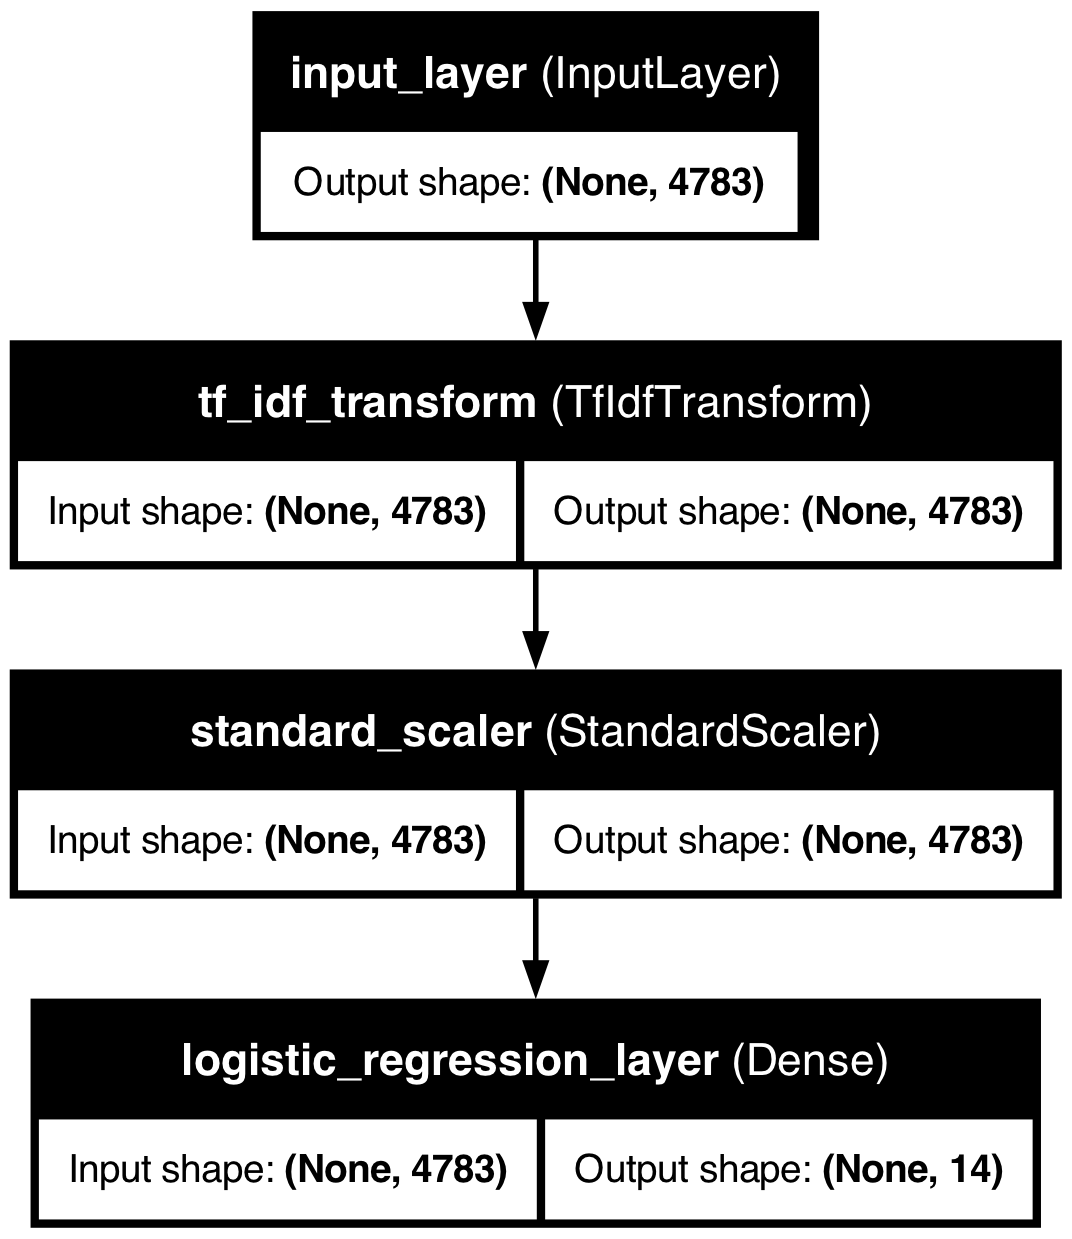
\includegraphics[keepaspectratio]{figures/model_pipeline.png}}

}

\caption{Model pipeline for deployment using tensorflow}

\end{figure}%

After deployment, model performance is monitored on Kibana using
ElasticSearch in our production environments (Elastic, 2025). With the
continuous inflow of student data and administrator responses, the model
will be continuously monitored and tuned with new data in order to adapt
to the real-world data distribution while improving model precision and
recall metrics.

\section{Results}\label{results}

\subsection{Data Collection}\label{data-collection-1}

During the initial phase of data relabeling, we discovered that there
was insufficient data for the categories Abortion, Drugs, Gambling,
Selfharm, Tobacco, and Weapons. The script, using the list of keywords
generated by permuting keywords related to the topic at hand, allowed us
to extract roughly 100 URLs per keyword, resulting in significant gains
for URL count.

\begin{longtable}[]{@{}ll@{}}
\caption{Unfiltered URLs collected with Selenium script.}\tabularnewline
\toprule\noalign{}
Category & New URLs collected as of 05/2025 \\
\midrule\noalign{}
\endfirsthead
\toprule\noalign{}
Category & New URLs collected as of 05/2025 \\
\midrule\noalign{}
\endhead
\bottomrule\noalign{}
\endlastfoot
Abortion & 14,056 \\
Drugs & 4,600 \\
Gambling & 4,287 \\
Self-harm & 4,859 \\
Tobacco & 2,248 \\
Weapons & 2,482 \\
\end{longtable}

However, as it is difficult to ascertain whether the URLs collected are
of good quality, we still had to manually relabel each individual URL
that we were going to use. Out of the additional 3'408 URLs collected
and screened both by LLM and hand, an additional 2'460 URLs were marked
as relevant and added to the existing database of URLs.

\begin{longtable}[]{@{}lll@{}}
\caption{Valid URLs after labeling.}\tabularnewline
\toprule\noalign{}
Topic & Host Count & URL Count \\
\midrule\noalign{}
\endfirsthead
\toprule\noalign{}
Topic & Host Count & URL Count \\
\midrule\noalign{}
\endhead
\bottomrule\noalign{}
\endlastfoot
Abortion & 26 & 311 \\
Drugs & 52 & 332 \\
Gambling & 172 & 235 \\
Self-harm & 7 & 337 \\
Tobacco & 135 & 272 \\
Weapon & 57 & 344 \\
\end{longtable}

\begin{figure}[H]

{\centering \pandocbounded{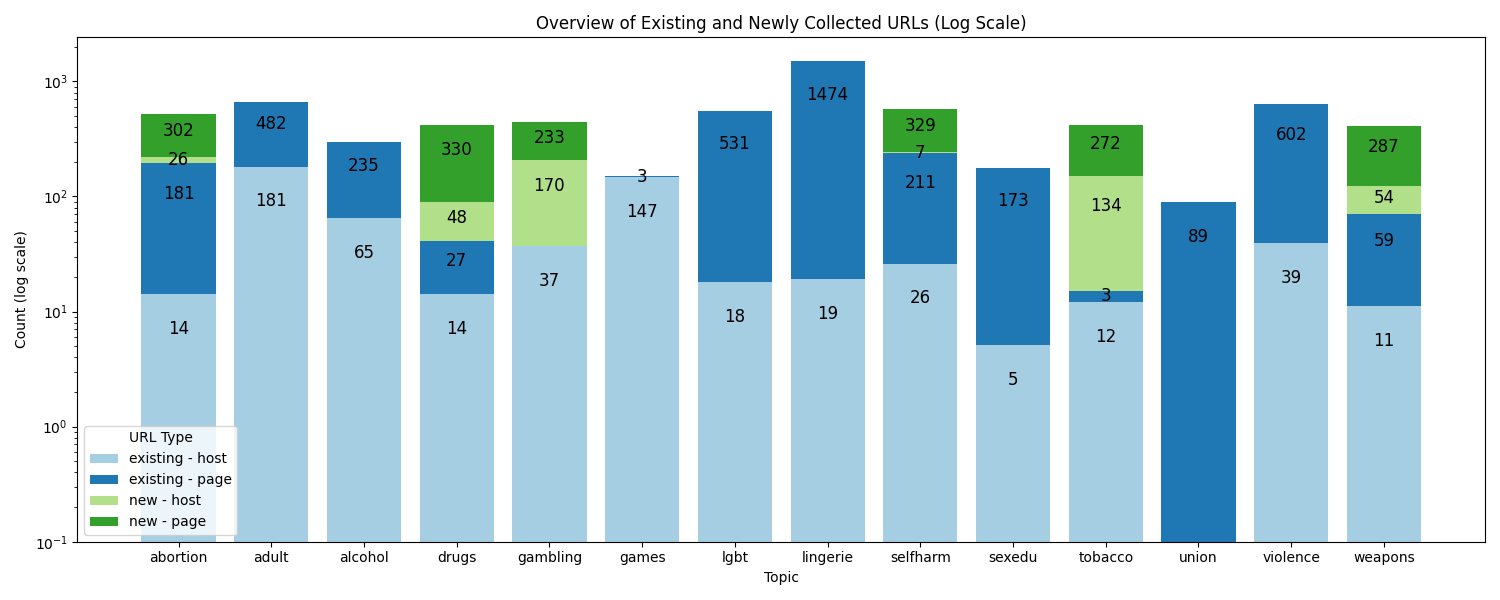
\includegraphics[keepaspectratio]{figures/1_url_collection_summary.png}}

}

\caption{Overview of all black URLs after additional collection period.}

\end{figure}%

\begin{longtable}[]{@{}lll@{}}
\caption{Summary of all valid URLs by category and type.}\tabularnewline
\toprule\noalign{}
Topic & Hosts & Pages \\
\midrule\noalign{}
\endfirsthead
\toprule\noalign{}
Topic & Hosts & Pages \\
\midrule\noalign{}
\endhead
\bottomrule\noalign{}
\endlastfoot
Abortion & 40 & 483 \\
Adult & 181 & 482 \\
Alcohol & 65 & 235 \\
Drugs & 62 & 357 \\
Gambling & 207 & 233 \\
Games & 147 & 3 \\
LGBT & 18 & 531 \\
Lingerie & 19 & 1474 \\
Self-harm & 33 & 540 \\
Sexedu & 5 & 173 \\
Tobacco & 146 & 275 \\
Violence & 39 & 602 \\
Weapons & 65 & 346 \\
\end{longtable}

The harmful/black URLs were crawled for content using the echo server
and parsed to text format, making up the datapoints in our dataset.
After crawling, our final dataset was created by taking the union of the
previous dataset and the current dataset, combining and removing the
duplicate black texts and appending the harmless (white) text to the
current dataset. The result is a modest dataset (\textasciitilde2.54 GB
in compressed format, \textasciitilde11.08 GB after decompression) with
412'984 non-null entries and 76.10\% of the data belonging to the white
category.

\begin{figure}[H]

{\centering \pandocbounded{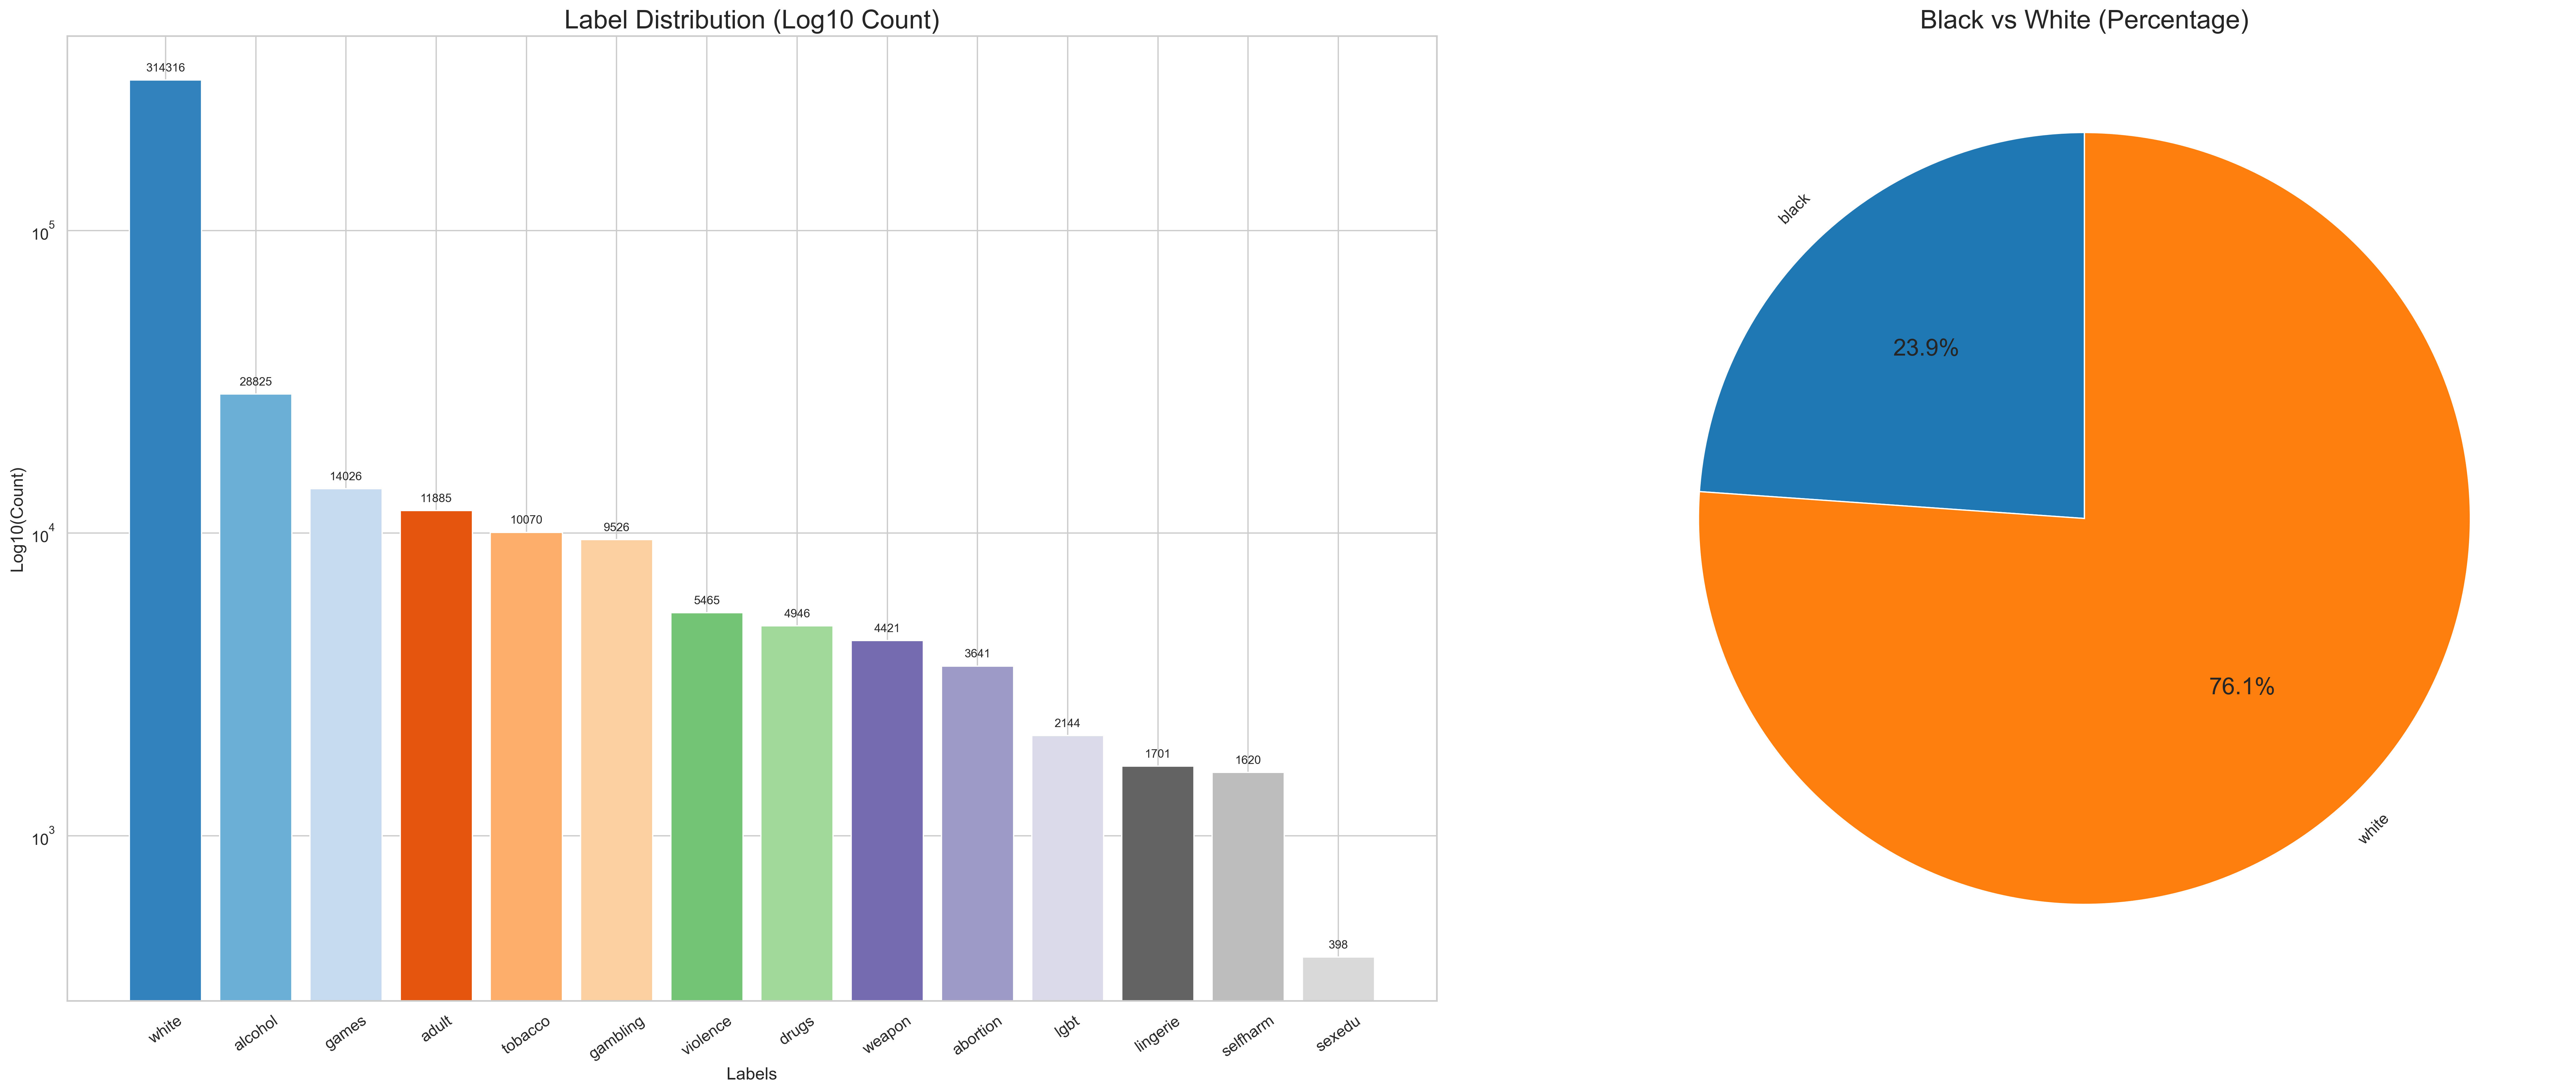
\includegraphics[keepaspectratio]{figures/2_label_distribution_all.png}}

}

\caption{Distribution of data points by category; percentage of data by
black/white categories.}

\end{figure}%

\begin{figure}[H]

{\centering \pandocbounded{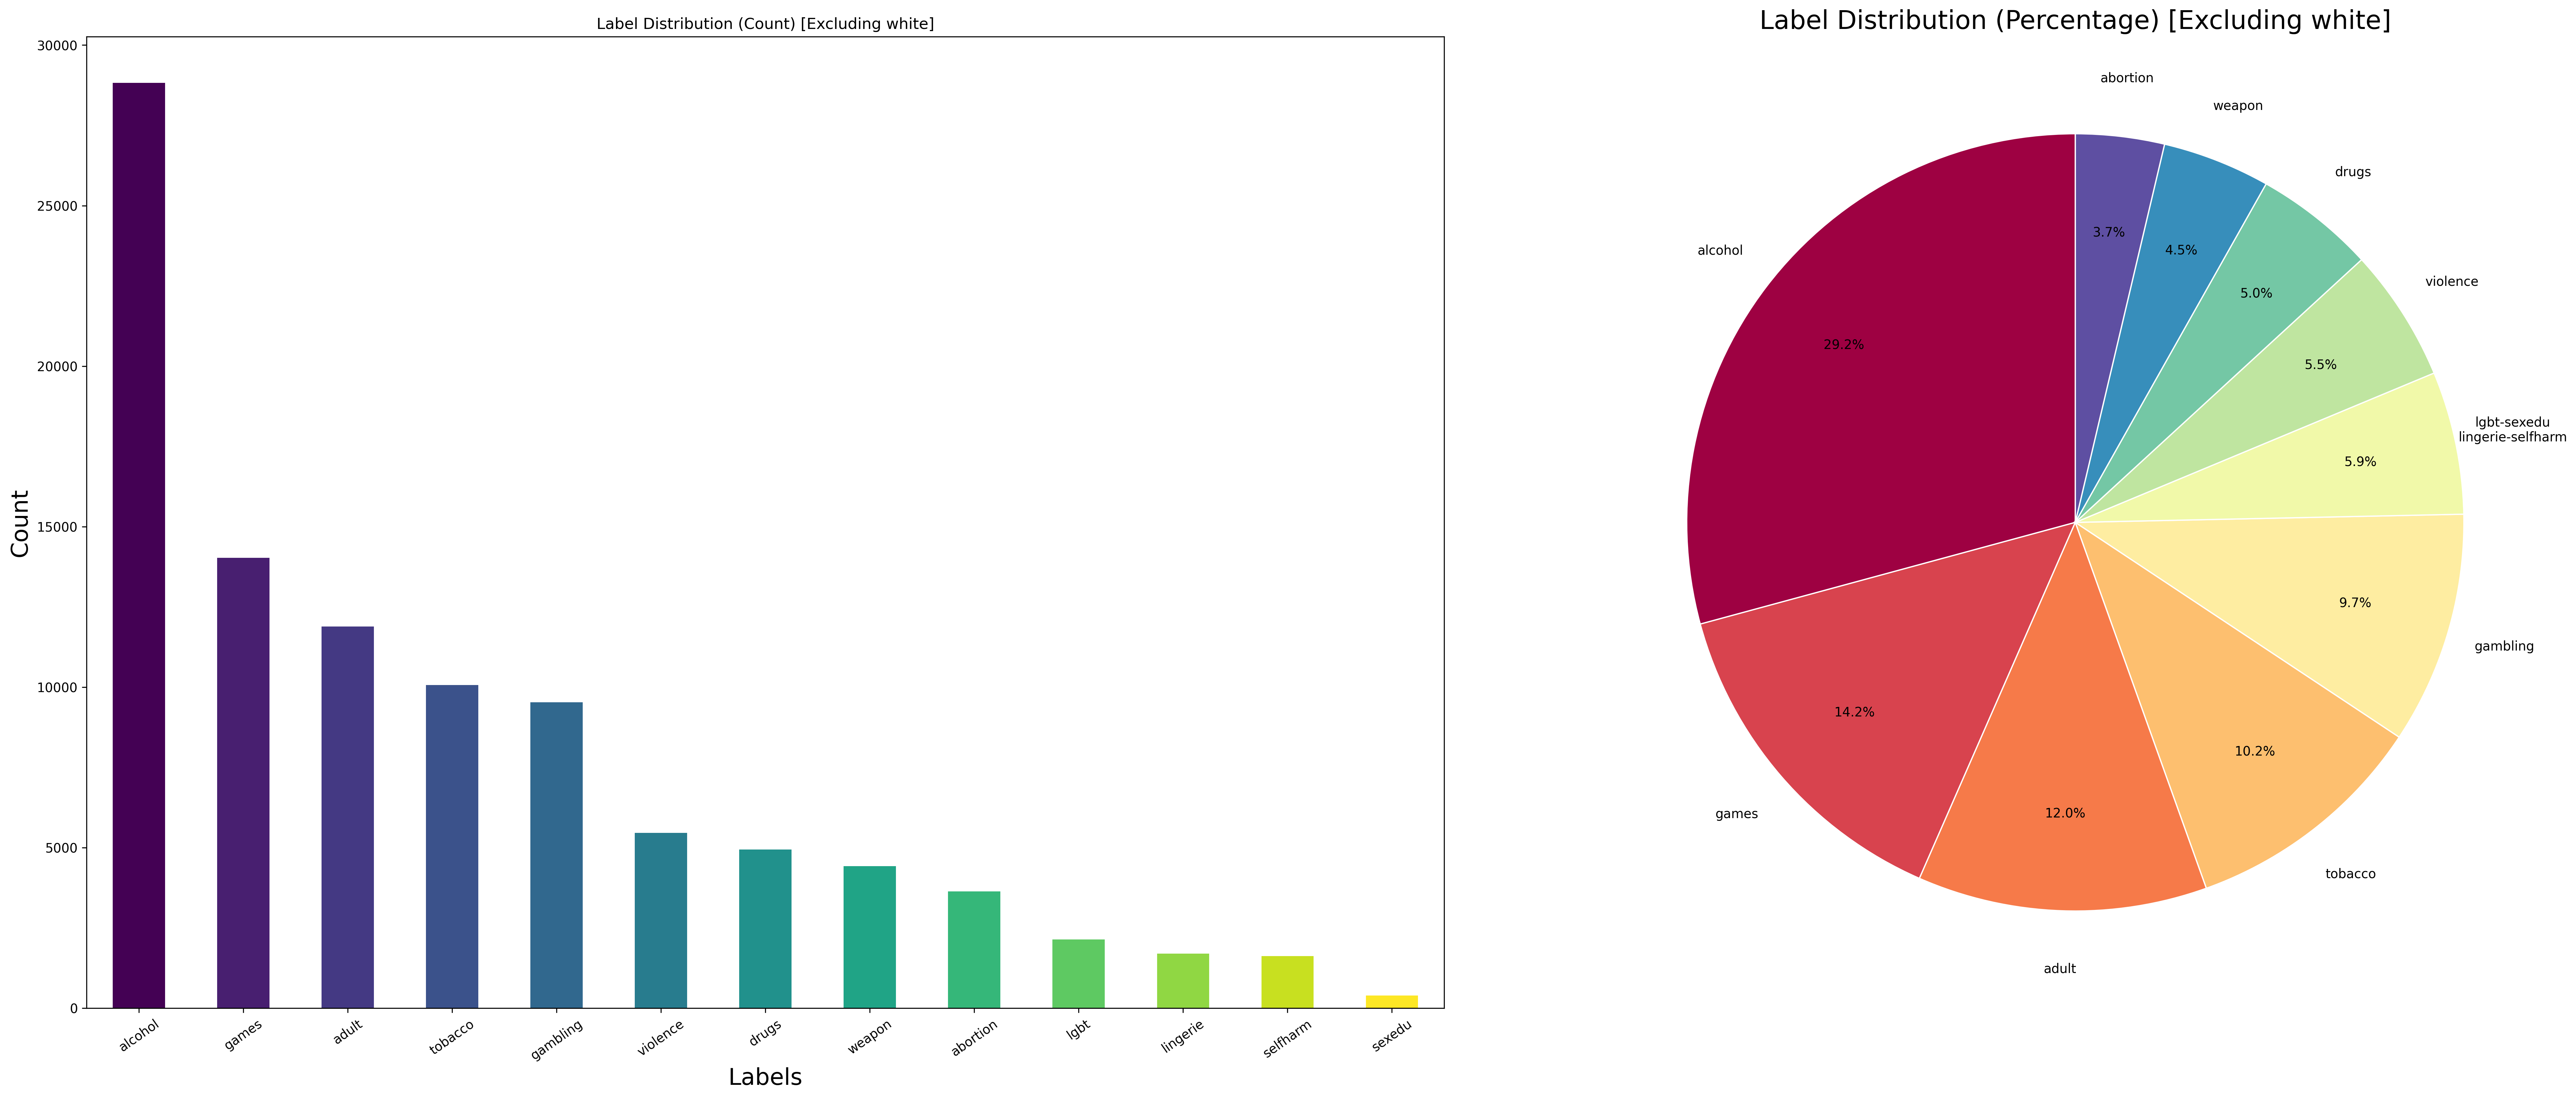
\includegraphics[keepaspectratio]{figures/3_label_distribution_no_white.png}}

}

\caption{Barplot/Pie Chart distribution of black text (note: LGBT,
Lingerie, Selfharm, and Sexedu were combined in the Pie Chart for a
concise representation).}

\end{figure}%

As we zoom in on the black data, we see that alcohol contains the most
data points out of all black categories with 28,825 datapoints, double
the number of datapoints from the next category down. The four
categories down from alcohol are games, adult, tobacco, and gambling,
all hovering around or above the 10 datapoint mark. Rounding off the
bottom 3 categories are lingerie (1701), selfharm (1620), and sexed
(398).

\begin{longtable}[]{@{}ll@{}}
\caption{Count of data points by category.}\tabularnewline
\toprule\noalign{}
Label & Distribution \\
\midrule\noalign{}
\endfirsthead
\toprule\noalign{}
Label & Distribution \\
\midrule\noalign{}
\endhead
\bottomrule\noalign{}
\endlastfoot
white & 314,316 \\
alcohol & 28,825 \\
games & 14,026 \\
adult & 11,885 \\
tobacco & 10,070 \\
gambling & 9,526 \\
violence & 5,465 \\
drugs & 4,946 \\
weapon & 4,421 \\
abortion & 3,641 \\
lgbt & 2,144 \\
lingerie & 1,701 \\
selfharm & 1,620 \\
sexedu & 398 \\
\end{longtable}

\begin{figure}[H]

{\centering \pandocbounded{\includegraphics[keepaspectratio]{figures/4_text_length_distributions.png}}

}

\caption{Histogram plot of unprocessed text length, unprocessed sentence
count, segmented/processed word count, and boxplot of text length by
category.}

\end{figure}%

Taking a closer look at the unprocessed and segmented text data, we see
that most text samples have a sentence count of up to 2500-3000 words,
with the distribution of the data resembling a rather skewed, almost
poisson distribution. Before stopwords are removed, sentences have up to
12'000 words per datapoint, that number decreasing to roughly 10'000
after segmentation using Jieba. In the box plot, we can see that most
data points contain roughly anywhere between 1'000-10'000 characters on
average and rarely exceed that range, meaning that most data points
collected contain a usable amount of data that can be further processed
and vectorized. For further details on text distribution, please refer
to the tables below.

\begin{longtable}[]{@{}
  >{\raggedright\arraybackslash}p{(\linewidth - 16\tabcolsep) * \real{0.1351}}
  >{\raggedright\arraybackslash}p{(\linewidth - 16\tabcolsep) * \real{0.1351}}
  >{\raggedright\arraybackslash}p{(\linewidth - 16\tabcolsep) * \real{0.1216}}
  >{\raggedright\arraybackslash}p{(\linewidth - 16\tabcolsep) * \real{0.1216}}
  >{\raggedright\arraybackslash}p{(\linewidth - 16\tabcolsep) * \real{0.0811}}
  >{\raggedright\arraybackslash}p{(\linewidth - 16\tabcolsep) * \real{0.0946}}
  >{\raggedright\arraybackslash}p{(\linewidth - 16\tabcolsep) * \real{0.0946}}
  >{\raggedright\arraybackslash}p{(\linewidth - 16\tabcolsep) * \real{0.0946}}
  >{\raggedright\arraybackslash}p{(\linewidth - 16\tabcolsep) * \real{0.1216}}@{}}
\caption{Text length statistics by category.}\tabularnewline
\toprule\noalign{}
\begin{minipage}[b]{\linewidth}\raggedright
Label
\end{minipage} & \begin{minipage}[b]{\linewidth}\raggedright
Count
\end{minipage} & \begin{minipage}[b]{\linewidth}\raggedright
Mean
\end{minipage} & \begin{minipage}[b]{\linewidth}\raggedright
Std Dev
\end{minipage} & \begin{minipage}[b]{\linewidth}\raggedright
Min
\end{minipage} & \begin{minipage}[b]{\linewidth}\raggedright
25\%
\end{minipage} & \begin{minipage}[b]{\linewidth}\raggedright
50\%
\end{minipage} & \begin{minipage}[b]{\linewidth}\raggedright
75\%
\end{minipage} & \begin{minipage}[b]{\linewidth}\raggedright
Max
\end{minipage} \\
\midrule\noalign{}
\endfirsthead
\toprule\noalign{}
\begin{minipage}[b]{\linewidth}\raggedright
Label
\end{minipage} & \begin{minipage}[b]{\linewidth}\raggedright
Count
\end{minipage} & \begin{minipage}[b]{\linewidth}\raggedright
Mean
\end{minipage} & \begin{minipage}[b]{\linewidth}\raggedright
Std Dev
\end{minipage} & \begin{minipage}[b]{\linewidth}\raggedright
Min
\end{minipage} & \begin{minipage}[b]{\linewidth}\raggedright
25\%
\end{minipage} & \begin{minipage}[b]{\linewidth}\raggedright
50\%
\end{minipage} & \begin{minipage}[b]{\linewidth}\raggedright
75\%
\end{minipage} & \begin{minipage}[b]{\linewidth}\raggedright
Max
\end{minipage} \\
\midrule\noalign{}
\endhead
\bottomrule\noalign{}
\endlastfoot
abortion & 3641.0 & 6709.99 & 3915.70 & 104.0 & 2480.0 & 7024.0 &
10236.0 & 15901.0 \\
adult & 11885.0 & 3389.30 & 2439.68 & 102.0 & 1432.0 & 2899.0 & 4708.0 &
13017.0 \\
alcohol & 28825.0 & 5252.35 & 3611.40 & 100.0 & 2310.0 & 4007.0 & 9412.0
& 12549.0 \\
drugs & 4946.0 & 4904.20 & 2924.90 & 111.0 & 2724.0 & 4411.5 & 6318.0 &
13839.0 \\
gambling & 9526.0 & 3744.82 & 2675.06 & 105.0 & 1748.5 & 3174.0 & 4708.0
& 12950.0 \\
games & 14026.0 & 3475.50 & 2189.05 & 106.0 & 1992.25 & 2975.0 & 4522.75
& 12461.0 \\
lgbt & 2144.0 & 3047.85 & 2236.94 & 111.0 & 1299.0 & 2586.5 & 4299.0 &
12374.0 \\
lingerie & 1701.0 & 3146.06 & 1997.06 & 100.0 & 1554.0 & 2982.0 & 4509.0
& 11296.0 \\
selfharm & 1620.0 & 2736.99 & 2066.88 & 136.0 & 1244.0 & 2004.0 & 3821.5
& 12816.0 \\
sexedu & 398.0 & 3138.07 & 1941.70 & 130.0 & 2114.25 & 2845.5 & 3801.25
& 11934.0 \\
tobacco & 10070.0 & 5453.66 & 3483.81 & 101.0 & 2674.25 & 4543.0 &
8769.75 & 12716.0 \\
violence & 5465.0 & 6089.82 & 3337.75 & 105.0 & 3005.0 & 5802.0 & 9336.0
& 12387.0 \\
weapon & 4421.0 & 5745.53 & 3504.39 & 130.0 & 2541.0 & 4974.0 & 9333.0 &
14301.0 \\
white & 314316.0 & 4204.18 & 3678.12 & 100.0 & 1765.0 & 3481.0 & 5528.0
& 760072.0 \\
\end{longtable}

\begin{longtable}[]{@{}
  >{\raggedright\arraybackslash}p{(\linewidth - 16\tabcolsep) * \real{0.1408}}
  >{\raggedright\arraybackslash}p{(\linewidth - 16\tabcolsep) * \real{0.1408}}
  >{\raggedright\arraybackslash}p{(\linewidth - 16\tabcolsep) * \real{0.1127}}
  >{\raggedright\arraybackslash}p{(\linewidth - 16\tabcolsep) * \real{0.1268}}
  >{\raggedright\arraybackslash}p{(\linewidth - 16\tabcolsep) * \real{0.0704}}
  >{\raggedright\arraybackslash}p{(\linewidth - 16\tabcolsep) * \real{0.0986}}
  >{\raggedright\arraybackslash}p{(\linewidth - 16\tabcolsep) * \real{0.0986}}
  >{\raggedright\arraybackslash}p{(\linewidth - 16\tabcolsep) * \real{0.0986}}
  >{\raggedright\arraybackslash}p{(\linewidth - 16\tabcolsep) * \real{0.1127}}@{}}
\caption{Raw text length statistics by category.}\tabularnewline
\toprule\noalign{}
\begin{minipage}[b]{\linewidth}\raggedright
Label
\end{minipage} & \begin{minipage}[b]{\linewidth}\raggedright
Count
\end{minipage} & \begin{minipage}[b]{\linewidth}\raggedright
Mean
\end{minipage} & \begin{minipage}[b]{\linewidth}\raggedright
Std Dev
\end{minipage} & \begin{minipage}[b]{\linewidth}\raggedright
Min
\end{minipage} & \begin{minipage}[b]{\linewidth}\raggedright
25\%
\end{minipage} & \begin{minipage}[b]{\linewidth}\raggedright
50\%
\end{minipage} & \begin{minipage}[b]{\linewidth}\raggedright
75\%
\end{minipage} & \begin{minipage}[b]{\linewidth}\raggedright
Max
\end{minipage} \\
\midrule\noalign{}
\endfirsthead
\toprule\noalign{}
\begin{minipage}[b]{\linewidth}\raggedright
Label
\end{minipage} & \begin{minipage}[b]{\linewidth}\raggedright
Count
\end{minipage} & \begin{minipage}[b]{\linewidth}\raggedright
Mean
\end{minipage} & \begin{minipage}[b]{\linewidth}\raggedright
Std Dev
\end{minipage} & \begin{minipage}[b]{\linewidth}\raggedright
Min
\end{minipage} & \begin{minipage}[b]{\linewidth}\raggedright
25\%
\end{minipage} & \begin{minipage}[b]{\linewidth}\raggedright
50\%
\end{minipage} & \begin{minipage}[b]{\linewidth}\raggedright
75\%
\end{minipage} & \begin{minipage}[b]{\linewidth}\raggedright
Max
\end{minipage} \\
\midrule\noalign{}
\endhead
\bottomrule\noalign{}
\endlastfoot
abortion & 3641.0 & 1102.49 & 841.44 & 1.0 & 181.0 & 1054.0 & 1991.0 &
3002.0 \\
adult & 11885.0 & 430.67 & 320.18 & 2.0 & 202.0 & 372.0 & 593.0 &
3441.0 \\
alcohol & 28825.0 & 793.85 & 567.15 & 11.0 & 313.0 & 599.0 & 1323.0 &
2234.0 \\
drugs & 4946.0 & 668.25 & 501.40 & 10.0 & 263.0 & 581.0 & 866.75 &
2397.0 \\
gambling & 9526.0 & 411.21 & 445.44 & 2.0 & 146.0 & 281.0 & 470.0 &
5052.0 \\
games & 14026.0 & 416.83 & 297.77 & 2.0 & 233.0 & 357.0 & 506.0 &
2941.0 \\
lgbt & 2144.0 & 328.73 & 279.58 & 1.0 & 151.75 & 253.0 & 401.0 &
3354.0 \\
lingerie & 1701.0 & 409.06 & 271.78 & 1.0 & 192.0 & 401.0 & 592.0 &
1611.0 \\
selfharm & 1620.0 & 278.06 & 231.19 & 3.0 & 159.0 & 206.0 & 324.25 &
1806.0 \\
sexedu & 398.0 & 342.11 & 232.02 & 16.0 & 190.5 & 349.0 & 392.75 &
1754.0 \\
tobacco & 10070.0 & 861.14 & 657.20 & 5.0 & 319.0 & 663.0 & 1396.0 &
2762.0 \\
violence & 5465.0 & 930.16 & 598.08 & 3.0 & 335.0 & 876.0 & 1503.0 &
2158.0 \\
weapon & 4421.0 & 841.94 & 572.94 & 15.0 & 310.0 & 727.0 & 1424.0 &
2240.0 \\
white & 314316.0 & 565.48 & 483.99 & 0.0 & 202.0 & 388.0 & 781.0 &
4092.0 \\
\end{longtable}

\begin{longtable}[]{@{}
  >{\raggedright\arraybackslash}p{(\linewidth - 16\tabcolsep) * \real{0.1449}}
  >{\raggedright\arraybackslash}p{(\linewidth - 16\tabcolsep) * \real{0.1304}}
  >{\raggedright\arraybackslash}p{(\linewidth - 16\tabcolsep) * \real{0.1159}}
  >{\raggedright\arraybackslash}p{(\linewidth - 16\tabcolsep) * \real{0.1304}}
  >{\raggedright\arraybackslash}p{(\linewidth - 16\tabcolsep) * \real{0.0725}}
  >{\raggedright\arraybackslash}p{(\linewidth - 16\tabcolsep) * \real{0.1014}}
  >{\raggedright\arraybackslash}p{(\linewidth - 16\tabcolsep) * \real{0.1014}}
  >{\raggedright\arraybackslash}p{(\linewidth - 16\tabcolsep) * \real{0.1014}}
  >{\raggedright\arraybackslash}p{(\linewidth - 16\tabcolsep) * \real{0.1014}}@{}}
\caption{Sentence count statistics by category.}\tabularnewline
\toprule\noalign{}
\begin{minipage}[b]{\linewidth}\raggedright
Label
\end{minipage} & \begin{minipage}[b]{\linewidth}\raggedright
Count
\end{minipage} & \begin{minipage}[b]{\linewidth}\raggedright
Mean
\end{minipage} & \begin{minipage}[b]{\linewidth}\raggedright
Std Dev
\end{minipage} & \begin{minipage}[b]{\linewidth}\raggedright
Min
\end{minipage} & \begin{minipage}[b]{\linewidth}\raggedright
25\%
\end{minipage} & \begin{minipage}[b]{\linewidth}\raggedright
50\%
\end{minipage} & \begin{minipage}[b]{\linewidth}\raggedright
75\%
\end{minipage} & \begin{minipage}[b]{\linewidth}\raggedright
Max
\end{minipage} \\
\midrule\noalign{}
\endfirsthead
\toprule\noalign{}
\begin{minipage}[b]{\linewidth}\raggedright
Label
\end{minipage} & \begin{minipage}[b]{\linewidth}\raggedright
Count
\end{minipage} & \begin{minipage}[b]{\linewidth}\raggedright
Mean
\end{minipage} & \begin{minipage}[b]{\linewidth}\raggedright
Std Dev
\end{minipage} & \begin{minipage}[b]{\linewidth}\raggedright
Min
\end{minipage} & \begin{minipage}[b]{\linewidth}\raggedright
25\%
\end{minipage} & \begin{minipage}[b]{\linewidth}\raggedright
50\%
\end{minipage} & \begin{minipage}[b]{\linewidth}\raggedright
75\%
\end{minipage} & \begin{minipage}[b]{\linewidth}\raggedright
Max
\end{minipage} \\
\midrule\noalign{}
\endhead
\bottomrule\noalign{}
\endlastfoot
abortion & 3641.0 & 1685.08 & 902.47 & 32.0 & 1048.0 & 1952.0 & 2123.0 &
9295.0 \\
adult & 11885.0 & 1549.58 & 1229.17 & 17.0 & 595.0 & 1228.0 & 2195.0 &
7686.0 \\
alcohol & 28825.0 & 1790.69 & 1231.77 & 19.0 & 830.0 & 1380.0 & 2796.0 &
5429.0 \\
drugs & 4946.0 & 1690.11 & 1121.55 & 26.0 & 927.25 & 1428.5 & 2180.0 &
9408.0 \\
gambling & 9526.0 & 1533.26 & 1041.43 & 23.0 & 771.0 & 1210.0 & 1940.0 &
5052.0 \\
games & 14026.0 & 1467.12 & 978.33 & 21.0 & 710.0 & 1179.0 & 2056.0 &
4920.0 \\
lgbt & 2144.0 & 1338.59 & 967.40 & 18.0 & 621.0 & 1015.0 & 1873.0 &
4597.0 \\
lingerie & 1701.0 & 1284.71 & 842.12 & 20.0 & 580.0 & 1042.0 & 1820.0 &
4210.0 \\
selfharm & 1620.0 & 1107.33 & 786.25 & 19.0 & 515.0 & 880.0 & 1580.0 &
3975.0 \\
sexedu & 398.0 & 1256.41 & 803.29 & 22.0 & 585.0 & 1066.0 & 1740.0 &
3899.0 \\
tobacco & 10070.0 & 1628.47 & 1044.12 & 19.0 & 771.0 & 1279.0 & 2128.0 &
4897.0 \\
violence & 5465.0 & 1710.89 & 1052.17 & 18.0 & 811.0 & 1328.0 & 2207.0 &
5189.0 \\
weapon & 4421.0 & 1684.72 & 1089.21 & 20.0 & 790.0 & 1277.0 & 2165.0 &
5021.0 \\
white & 314316.0 & 1420.53 & 1007.39 & 15.0 & 650.0 & 1148.0 & 1959.0 &
4811.0 \\
\end{longtable}

\begin{figure}[H]

{\centering \pandocbounded{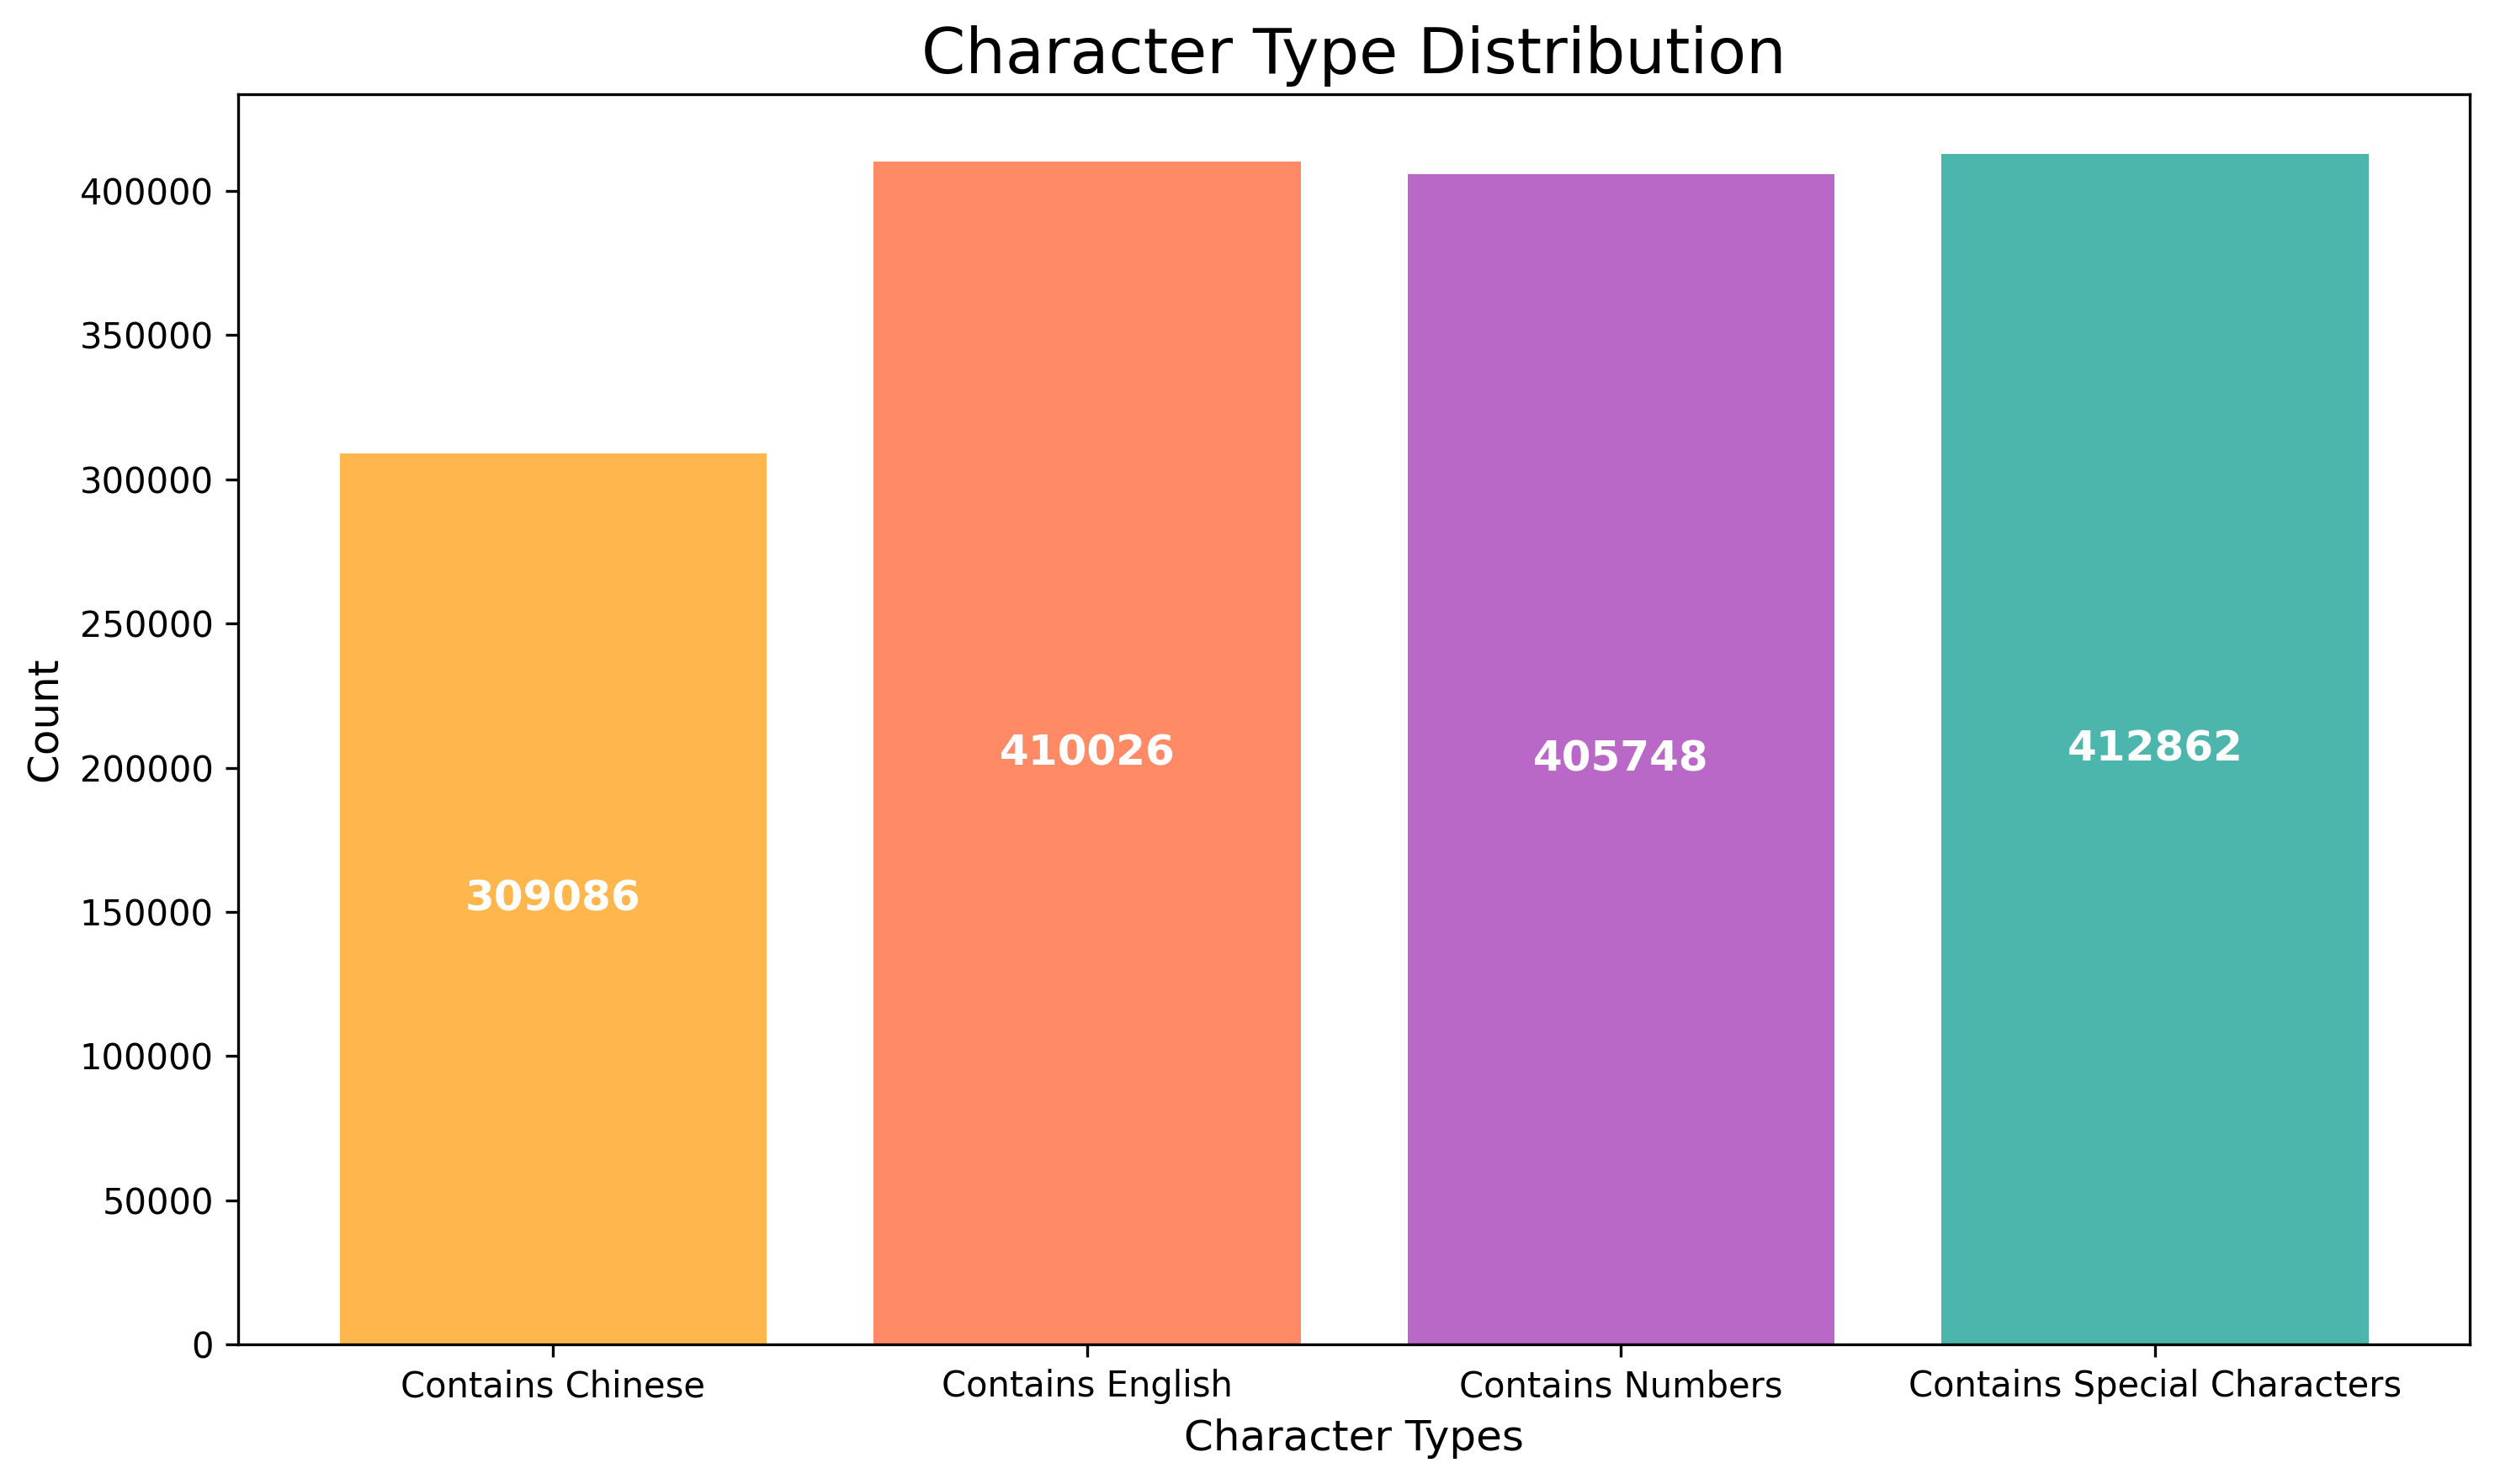
\includegraphics[keepaspectratio]{figures/5_character_type_distribution.png}}

}

\caption{Distribution of character types in the dataset, showing counts
of entries containing Chinese, English, numerical, and special
characters.}

\end{figure}%

It is interesting to note that with our dataset containing just over
400'000 datapoints, we only have roughly 309'000 datapoints that contain
Chinese. After further analysis, it seems that the white category
contains a number of datapoints from other languages, including but not
limited to English, Russian, Spanish, and other languages, accounting
for the discrepancy.

\subsection{Feature Extraction}\label{feature-extraction}

Initially, a trial run with 5'000, 10'000, and 12'000 features were
tried for a baseline LinearSVC model as a test, yet a more rigorous
method was needed for the TF-IDF vectorizer dictionary. Using both the
TF-IDF and textrank algorithm (both natively implemented in jieba), the
top 200 features from the individual categories were extracted and
compared. On average, the two methods produced rather diverging results,
where the average jaccard similarity is around 0.2743. The most similar
category, which just happens to be the category with the least number of
datapoints, had the highest Jaccard similarity of 0.434 while the
categories tobacco and weapon are tied for the lowest jaccard score of
0.190 each.

\begin{longtable}[]{@{}
  >{\raggedright\arraybackslash}p{(\linewidth - 8\tabcolsep) * \real{0.1111}}
  >{\raggedright\arraybackslash}p{(\linewidth - 8\tabcolsep) * \real{0.2111}}
  >{\raggedright\arraybackslash}p{(\linewidth - 8\tabcolsep) * \real{0.2222}}
  >{\raggedright\arraybackslash}p{(\linewidth - 8\tabcolsep) * \real{0.2222}}
  >{\raggedright\arraybackslash}p{(\linewidth - 8\tabcolsep) * \real{0.2333}}@{}}
\caption{Jaccard similarity between top 200 features
extracted.}\tabularnewline
\toprule\noalign{}
\begin{minipage}[b]{\linewidth}\raggedright
Category
\end{minipage} & \begin{minipage}[b]{\linewidth}\raggedright
Extract Tag Count
\end{minipage} & \begin{minipage}[b]{\linewidth}\raggedright
TextRank Tag Count
\end{minipage} & \begin{minipage}[b]{\linewidth}\raggedright
Intersection Count
\end{minipage} & \begin{minipage}[b]{\linewidth}\raggedright
Jaccard Similarity
\end{minipage} \\
\midrule\noalign{}
\endfirsthead
\toprule\noalign{}
\begin{minipage}[b]{\linewidth}\raggedright
Category
\end{minipage} & \begin{minipage}[b]{\linewidth}\raggedright
Extract Tag Count
\end{minipage} & \begin{minipage}[b]{\linewidth}\raggedright
TextRank Tag Count
\end{minipage} & \begin{minipage}[b]{\linewidth}\raggedright
Intersection Count
\end{minipage} & \begin{minipage}[b]{\linewidth}\raggedright
Jaccard Similarity
\end{minipage} \\
\midrule\noalign{}
\endhead
\bottomrule\noalign{}
\endlastfoot
abortion & 200 & 200 & 73 & 0.223 \\
adult & 200 & 200 & 91 & 0.294 \\
alcohol & 200 & 200 & 82 & 0.258 \\
drugs & 200 & 200 & 78 & 0.242 \\
gambling & 200 & 200 & 82 & 0.258 \\
games & 200 & 200 & 94 & 0.307 \\
lgbt & 200 & 200 & 95 & 0.311 \\
lingerie & 200 & 200 & 96 & 0.316 \\
selfharm & 200 & 200 & 73 & 0.223 \\
sexedu & 200 & 200 & 121 & 0.434 \\
tobacco & 200 & 200 & 64 & 0.190 \\
violence & 200 & 200 & 97 & 0.320 \\
weapon & 200 & 200 & 64 & 0.190 \\
\end{longtable}

Additionally, 2'400 features were extracted from the white category
using the TF-IDF method, which provided us with a theoretical maximum of
10'000 features. However, after taking the union of the resulting
textrank and TF-IDF dictionaries, we arrived at 2561 features for the
black category. Combined with 2'500 features (instead of 2'400 features)
extracted from the white category using TF-IDF as well as the additional
features extracted on a category-wide basis, we arrived at a final
TF-IDF dictionary size of 4'783.

\subsubsection{Topic Modelling}\label{topic-modelling}

During the process of topic modelling using Latent Dirichlet Allocation
(LDA), it was discovered that some topics and datapoints separated
themselves quite well after applying LDA such as Alcohol (Red), Games
(Purple), and Gambling (light pink).

\begin{figure}[H]

{\centering \pandocbounded{\includegraphics[keepaspectratio]{figures/6_lda_30topics.png}}

}

\caption{30 topics and T-SNE using \texttt{pca}.}

\end{figure}%

\begin{figure}[H]

{\centering \pandocbounded{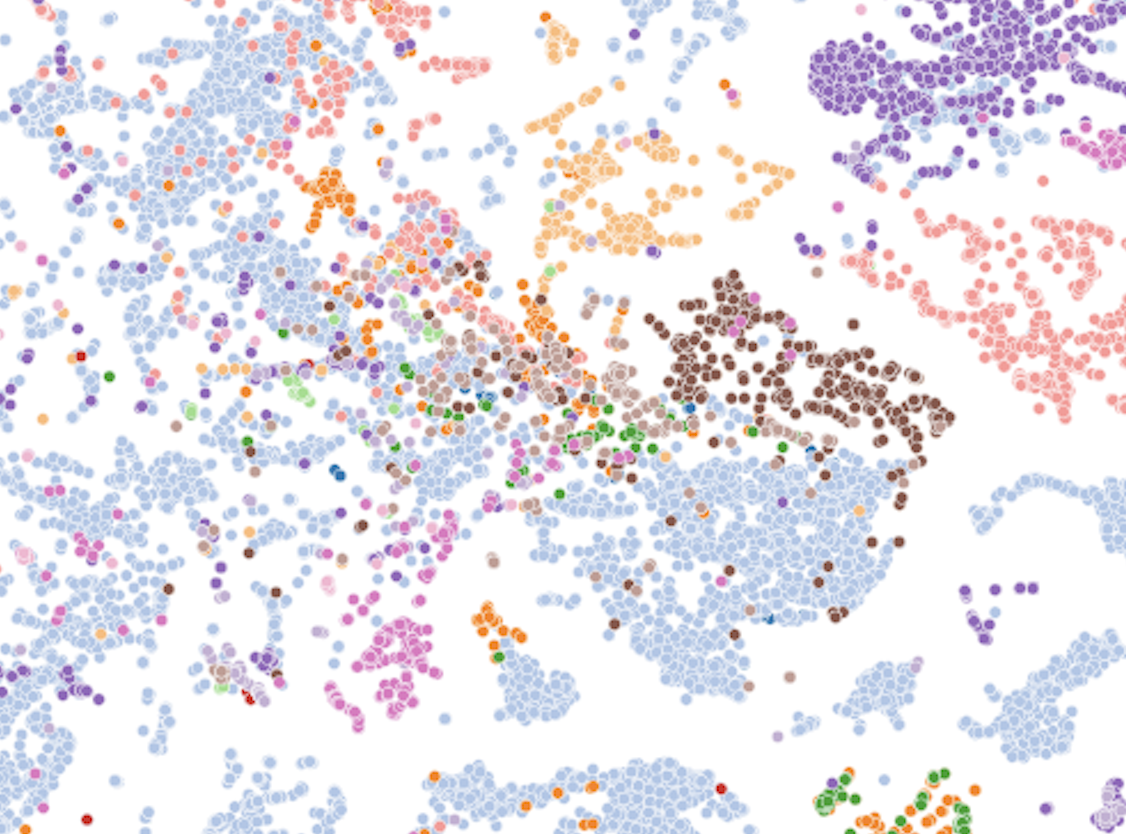
\includegraphics[keepaspectratio]{figures/9_1_150.png}}

}

\caption{Excerpt \#1 from LDA with 150 topics, with noticeable confusion
clusters between lgbt (dark green), selfharm (grey), drugs (orange),
gambling (salmon), adult (pink), and lingerie (light pink) after t-SNE
projection.}

\end{figure}%

\begin{figure}

\begin{minipage}{\linewidth}

\begin{figure}[H]

{\centering \pandocbounded{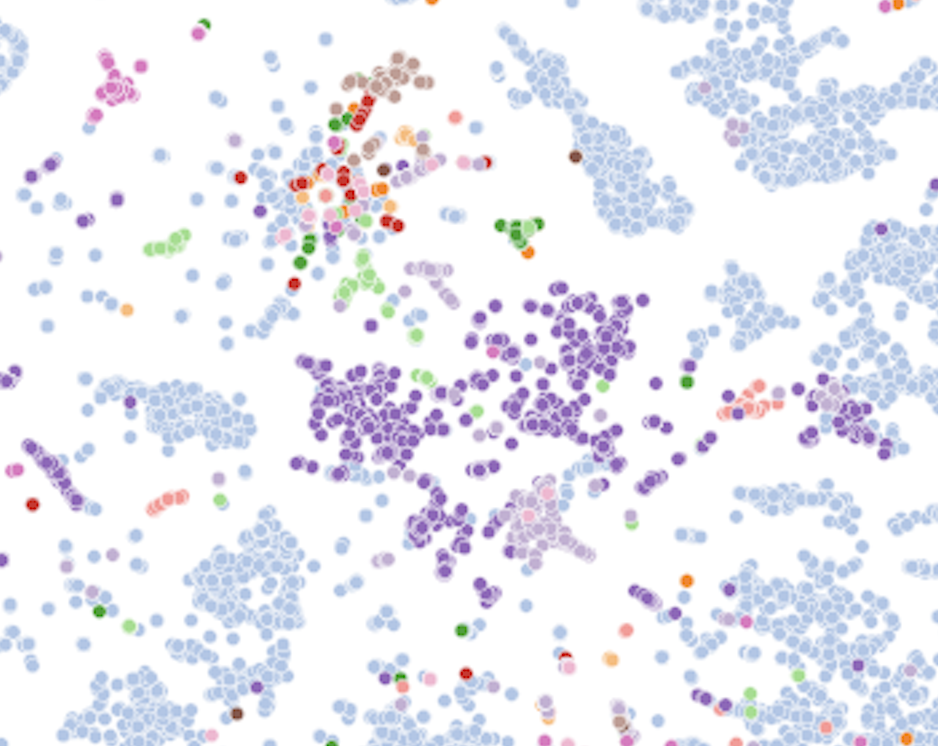
\includegraphics[keepaspectratio]{figures/9_2_150.png}}

}

\subcaption{Excerpt \#2 from LDA with 150 topics, with noticeable
confusion clusters between lgbt (dark green), alcohol (red), and
selfharm (brown), as well as between games (purple) and violence (light
purple) after t-SNE projection.}

\end{figure}%

\end{minipage}%
\newline
\begin{minipage}{\linewidth}

\begin{figure}[H]

{\centering \pandocbounded{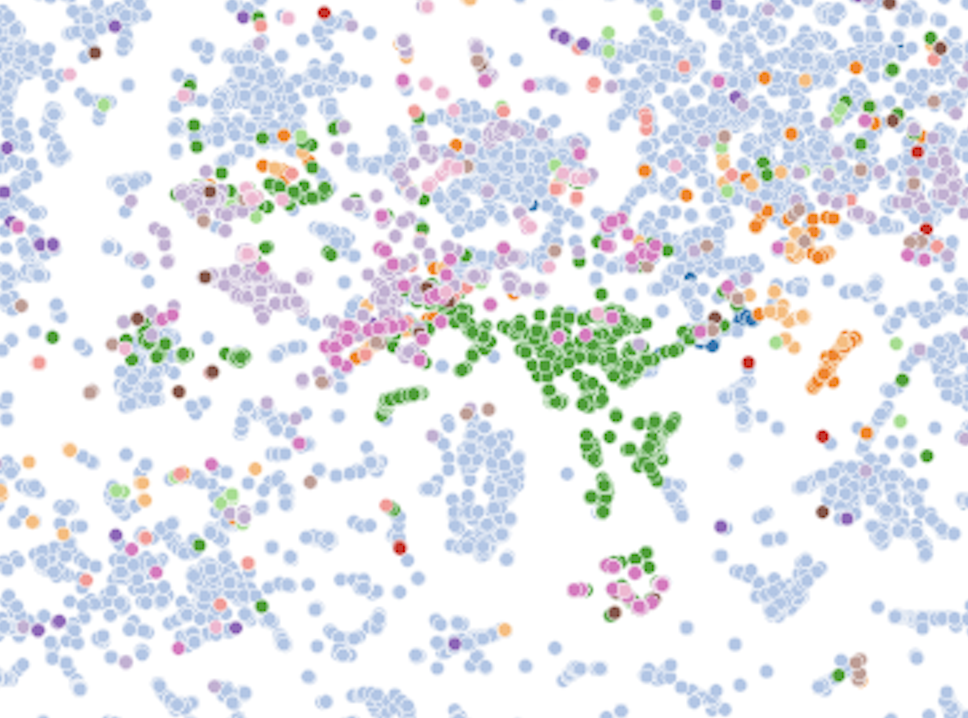
\includegraphics[keepaspectratio]{figures/9_3_150.png}}

}

\subcaption{Excerpt \#3 from LDA with 150 topics, with noticeable
confusion clusters between lgbt (dark green), adult (pink), and violence
(light purple) after t-SNE projection.}

\end{figure}%

\end{minipage}%

\end{figure}%

However, other topics are more difficult to separate, with many
localized clusters containing data points from multiple topics, such as
between games (purple) and violence (light purple), alcohol (red),
selfharm (light brown), lgbt (dark green) and tobacco (light orange), as
well as lgbt (dark green), adult (pink), and violence (light purple).

\subsection{Initial Model Selection}\label{initial-model-selection}

The result of evaluating the 30+ baseline model candidates showed that
linear models (logistic regression, linear support vectors, multilayer
perceptron, etc.) and boosted decision trees performed the best out of
all the models. It is also worth noting that certain methods
outperformed others when it comes to default parameter performance.

\begin{longtable}[]{@{}lllll@{}}
\caption{Best performing model by class.}\tabularnewline
\toprule\noalign{}
Class Name & Best Model & F1 Score & Precision & Recall \\
\midrule\noalign{}
\endfirsthead
\toprule\noalign{}
Class Name & Best Model & F1 Score & Precision & Recall \\
\midrule\noalign{}
\endhead
\bottomrule\noalign{}
\endlastfoot
abortion & RidgeClassifier & 0.871 & 0.846 & 0.897 \\
adult & PassiveAggressive & 0.967 & 0.964 & 0.970 \\
alcohol & ExtraTrees & 0.997 & 0.999 & 0.996 \\
drugs & SVC\_RBF & 0.871 & 0.894 & 0.850 \\
gambling & PassiveAggressive & 0.990 & 0.994 & 0.987 \\
games & PassiveAggressive & 0.986 & 0.985 & 0.988 \\
lgbt & RidgeClassifier & 0.834 & 0.960 & 0.737 \\
lingerie & PassiveAggressive & 0.938 & 0.946 & 0.929 \\
selfharm & XGBoost & 0.903 & 0.946 & 0.864 \\
sexedu & SGDClassifier & 0.947 & 1.000 & 0.900 \\
tobacco & PassiveAggressive & 0.992 & 0.991 & 0.994 \\
violence & XGBoost & 0.863 & 0.897 & 0.832 \\
weapon & XGBoost & 0.880 & 0.897 & 0.864 \\
white & PassiveAggressive & 0.997 & 0.997 & 0.998 \\
\end{longtable}

The best model was the passive aggressive classifier, a textbook linear
model implementation designed for large-scale learning using squared
hinge loss without the need of a learning rate. Similar to LinearSVC and
Logistic Regression, the passive aggressive classifier has a
regularization hyperparameter C. Nevertheless, Logistic Regression,
however, was the most balanced model out of all tested models with a
macro averaged F1-Score of 0.9062. In fact, most well-performing models
seem to hit a performance bottleneck around the 0.9 mark and don't seem
to improve much in terms of F1-macro performance.

\begin{figure}[H]

{\centering \pandocbounded{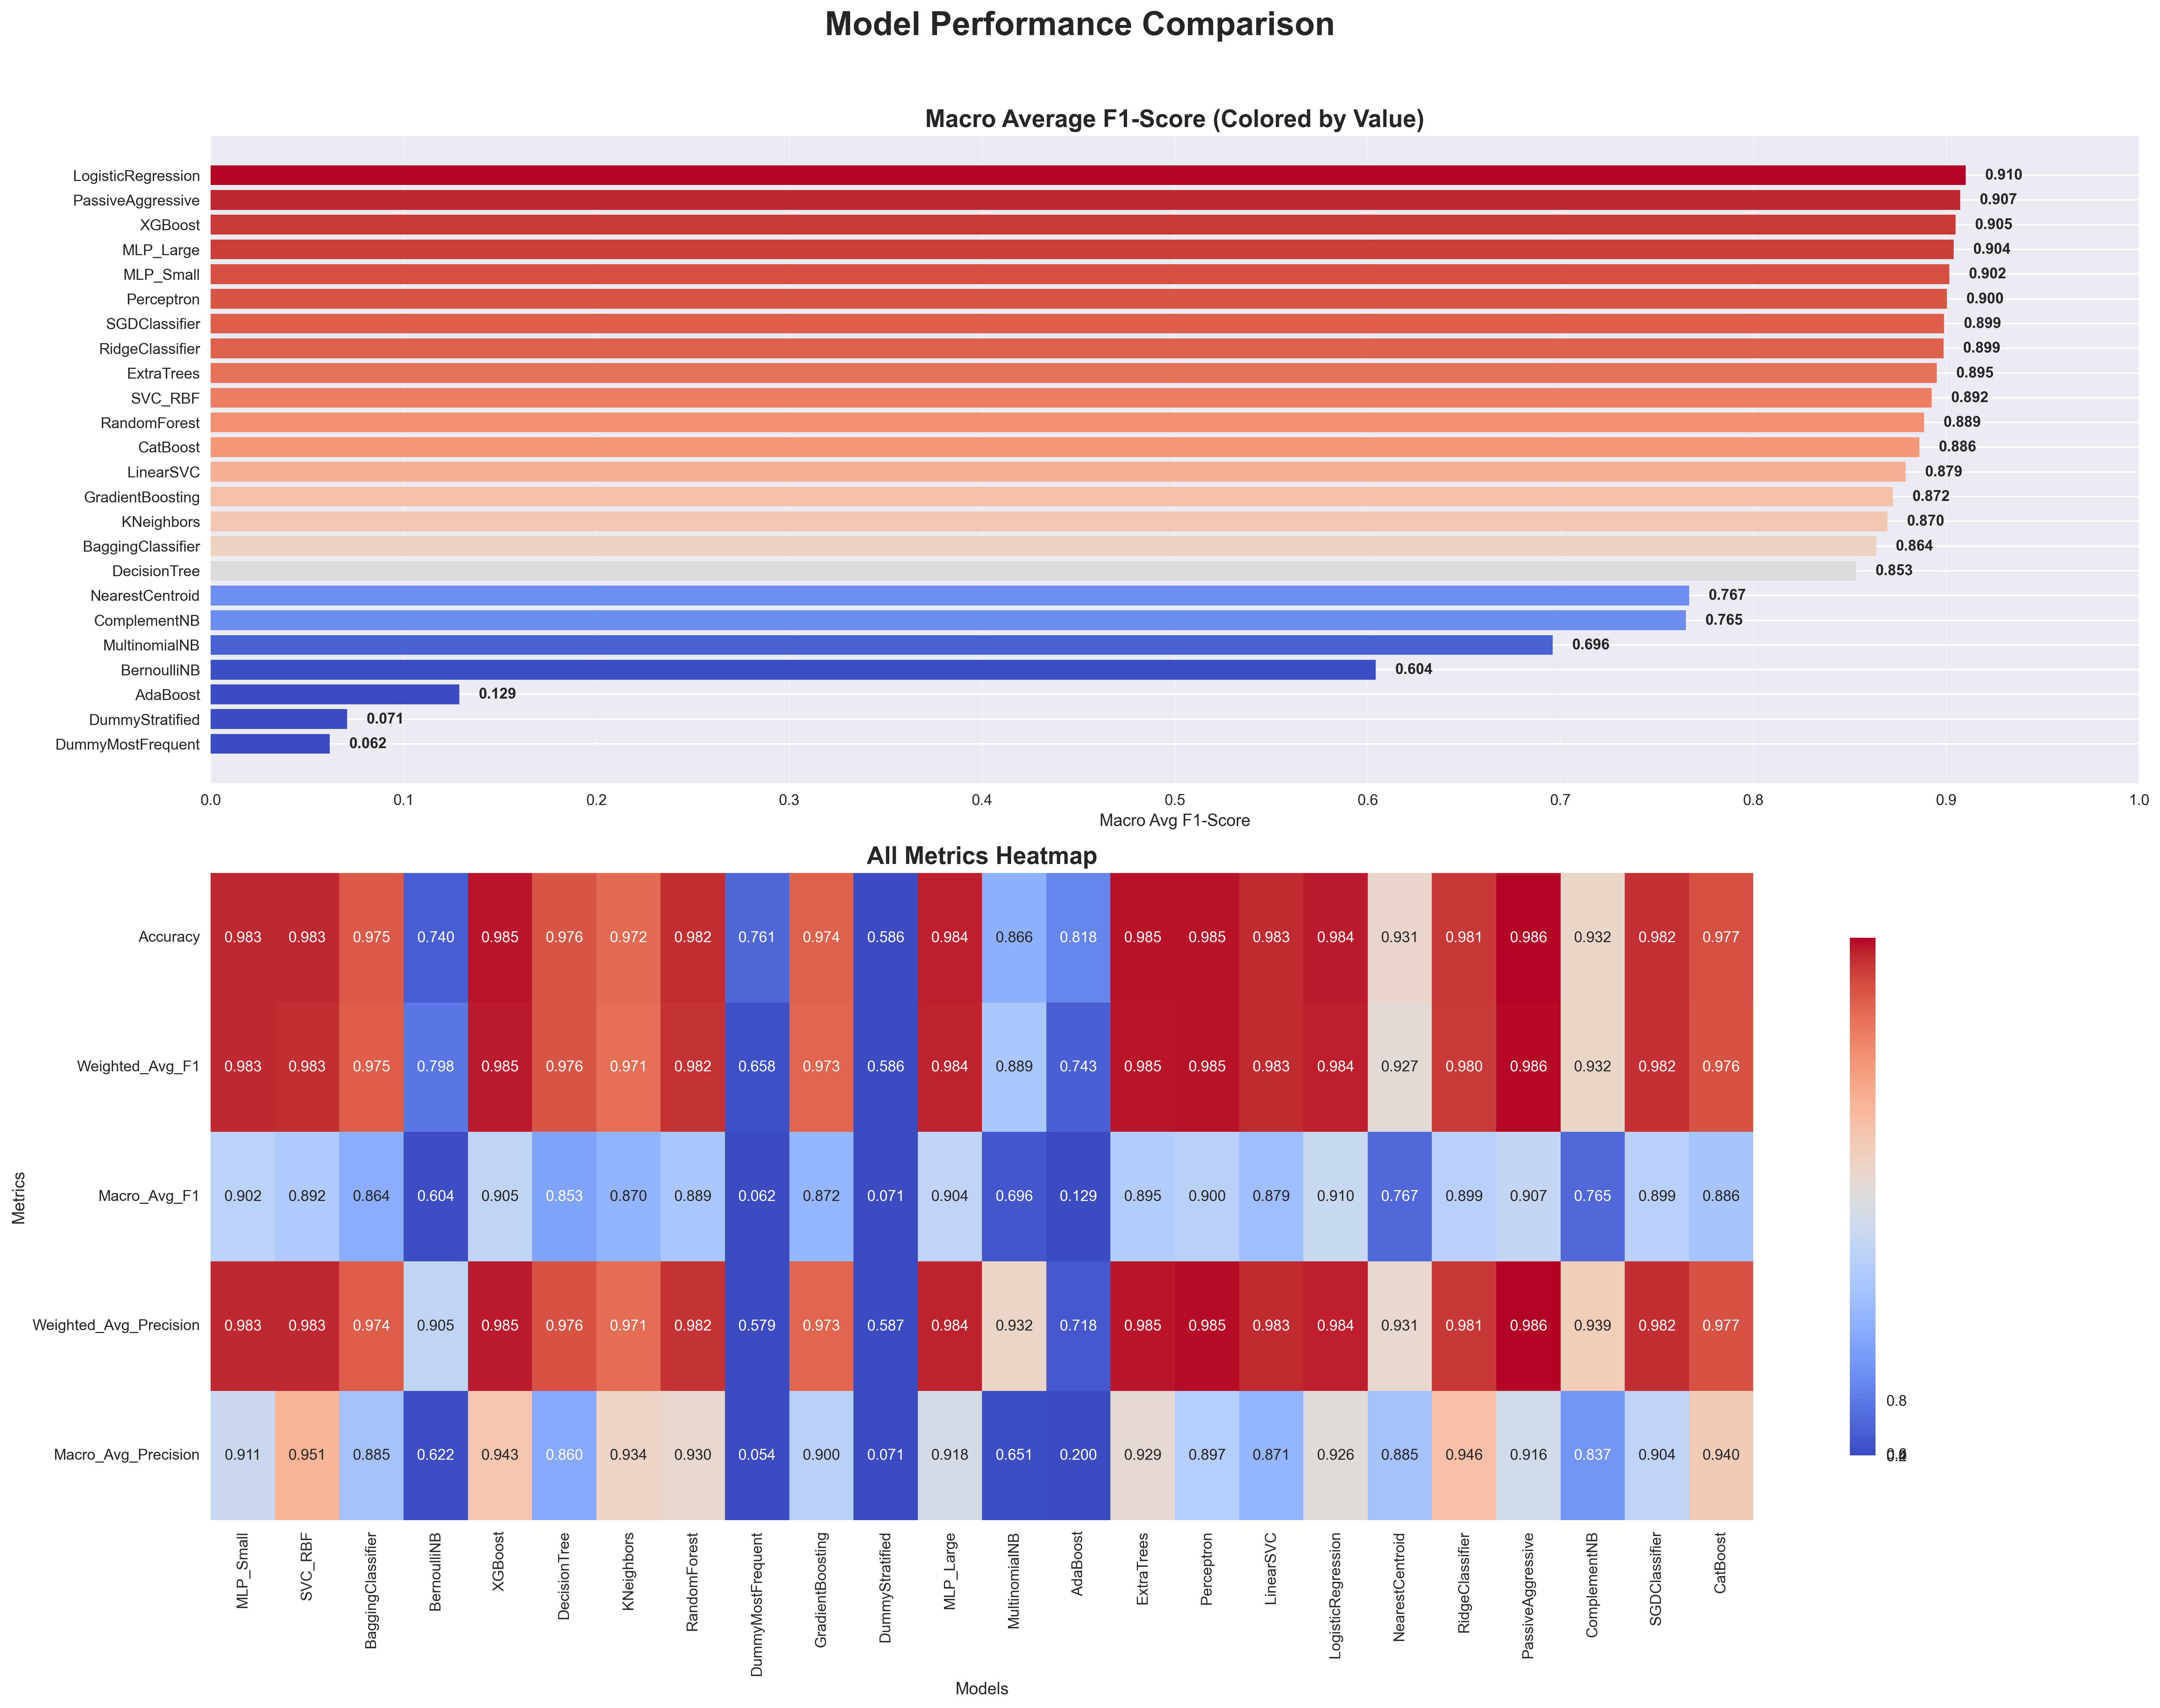
\includegraphics[keepaspectratio]{figures/10_simplified_performance_comparison.png}}

}

\caption{Comparison of all models by class.}

\end{figure}%

\begin{longtable}[]{@{}lll@{}}
\caption{Top 10 models ranked by accuracy.}\tabularnewline
\toprule\noalign{}
Model & Accuracy & Macro Avg F1 \\
\midrule\noalign{}
\endfirsthead
\toprule\noalign{}
Model & Accuracy & Macro Avg F1 \\
\midrule\noalign{}
\endhead
\bottomrule\noalign{}
\endlastfoot
PassiveAggressive & 0.986 & 0.907 \\
ExtraTrees & 0.985 & 0.895 \\
Perceptron & 0.985 & 0.900 \\
XGBoost & 0.985 & 0.905 \\
LogisticRegression & 0.984 & 0.910 \\
MLP\_Large & 0.984 & 0.904 \\
MLP\_Small & 0.983 & 0.902 \\
SVC\_RBF & 0.983 & 0.892 \\
LinearSVC & 0.983 & 0.879 \\
RandomForest & 0.982 & 0.889 \\
\end{longtable}

Based solely on accuracy and macro average F1-scores, the
best-performing model is PassiveAggressive, achieving the highest
accuracy of 0.986 and a strong macro F1 of 0.907, indicating both
overall precision and balanced class-wise performance. ExtraTrees,
Perceptron, and XGBoost follow closely with 0.985 accuracy, with XGBoost
showing the highest macro F1 among them at 0.905, suggesting more
consistent performance across classes. LogisticRegression stands out
with a macro F1 of 0.910--- the highest among all--- despite a slightly
lower accuracy of 0.984, reflecting excellent balance across class
predictions. The neural models, MLP\_Large and MLP\_Small, perform
comparably with accuracies of 0.984 and 0.983, and macro F1 scores of
0.904 and 0.902 respectively, indicating strong generalization. SVC\_RBF
and LinearSVC both achieve 0.983 accuracy, though LinearSVC lags in
macro F1 at 0.879. Lastly, RandomForest shows the lowest accuracy
(0.982) and a macro F1 of 0.889, still solid but slightly behind the
others. Overall, all models perform well, with minor trade-offs between
accuracy and macro-level F1 scores.

\begin{figure}[H]

{\centering \pandocbounded{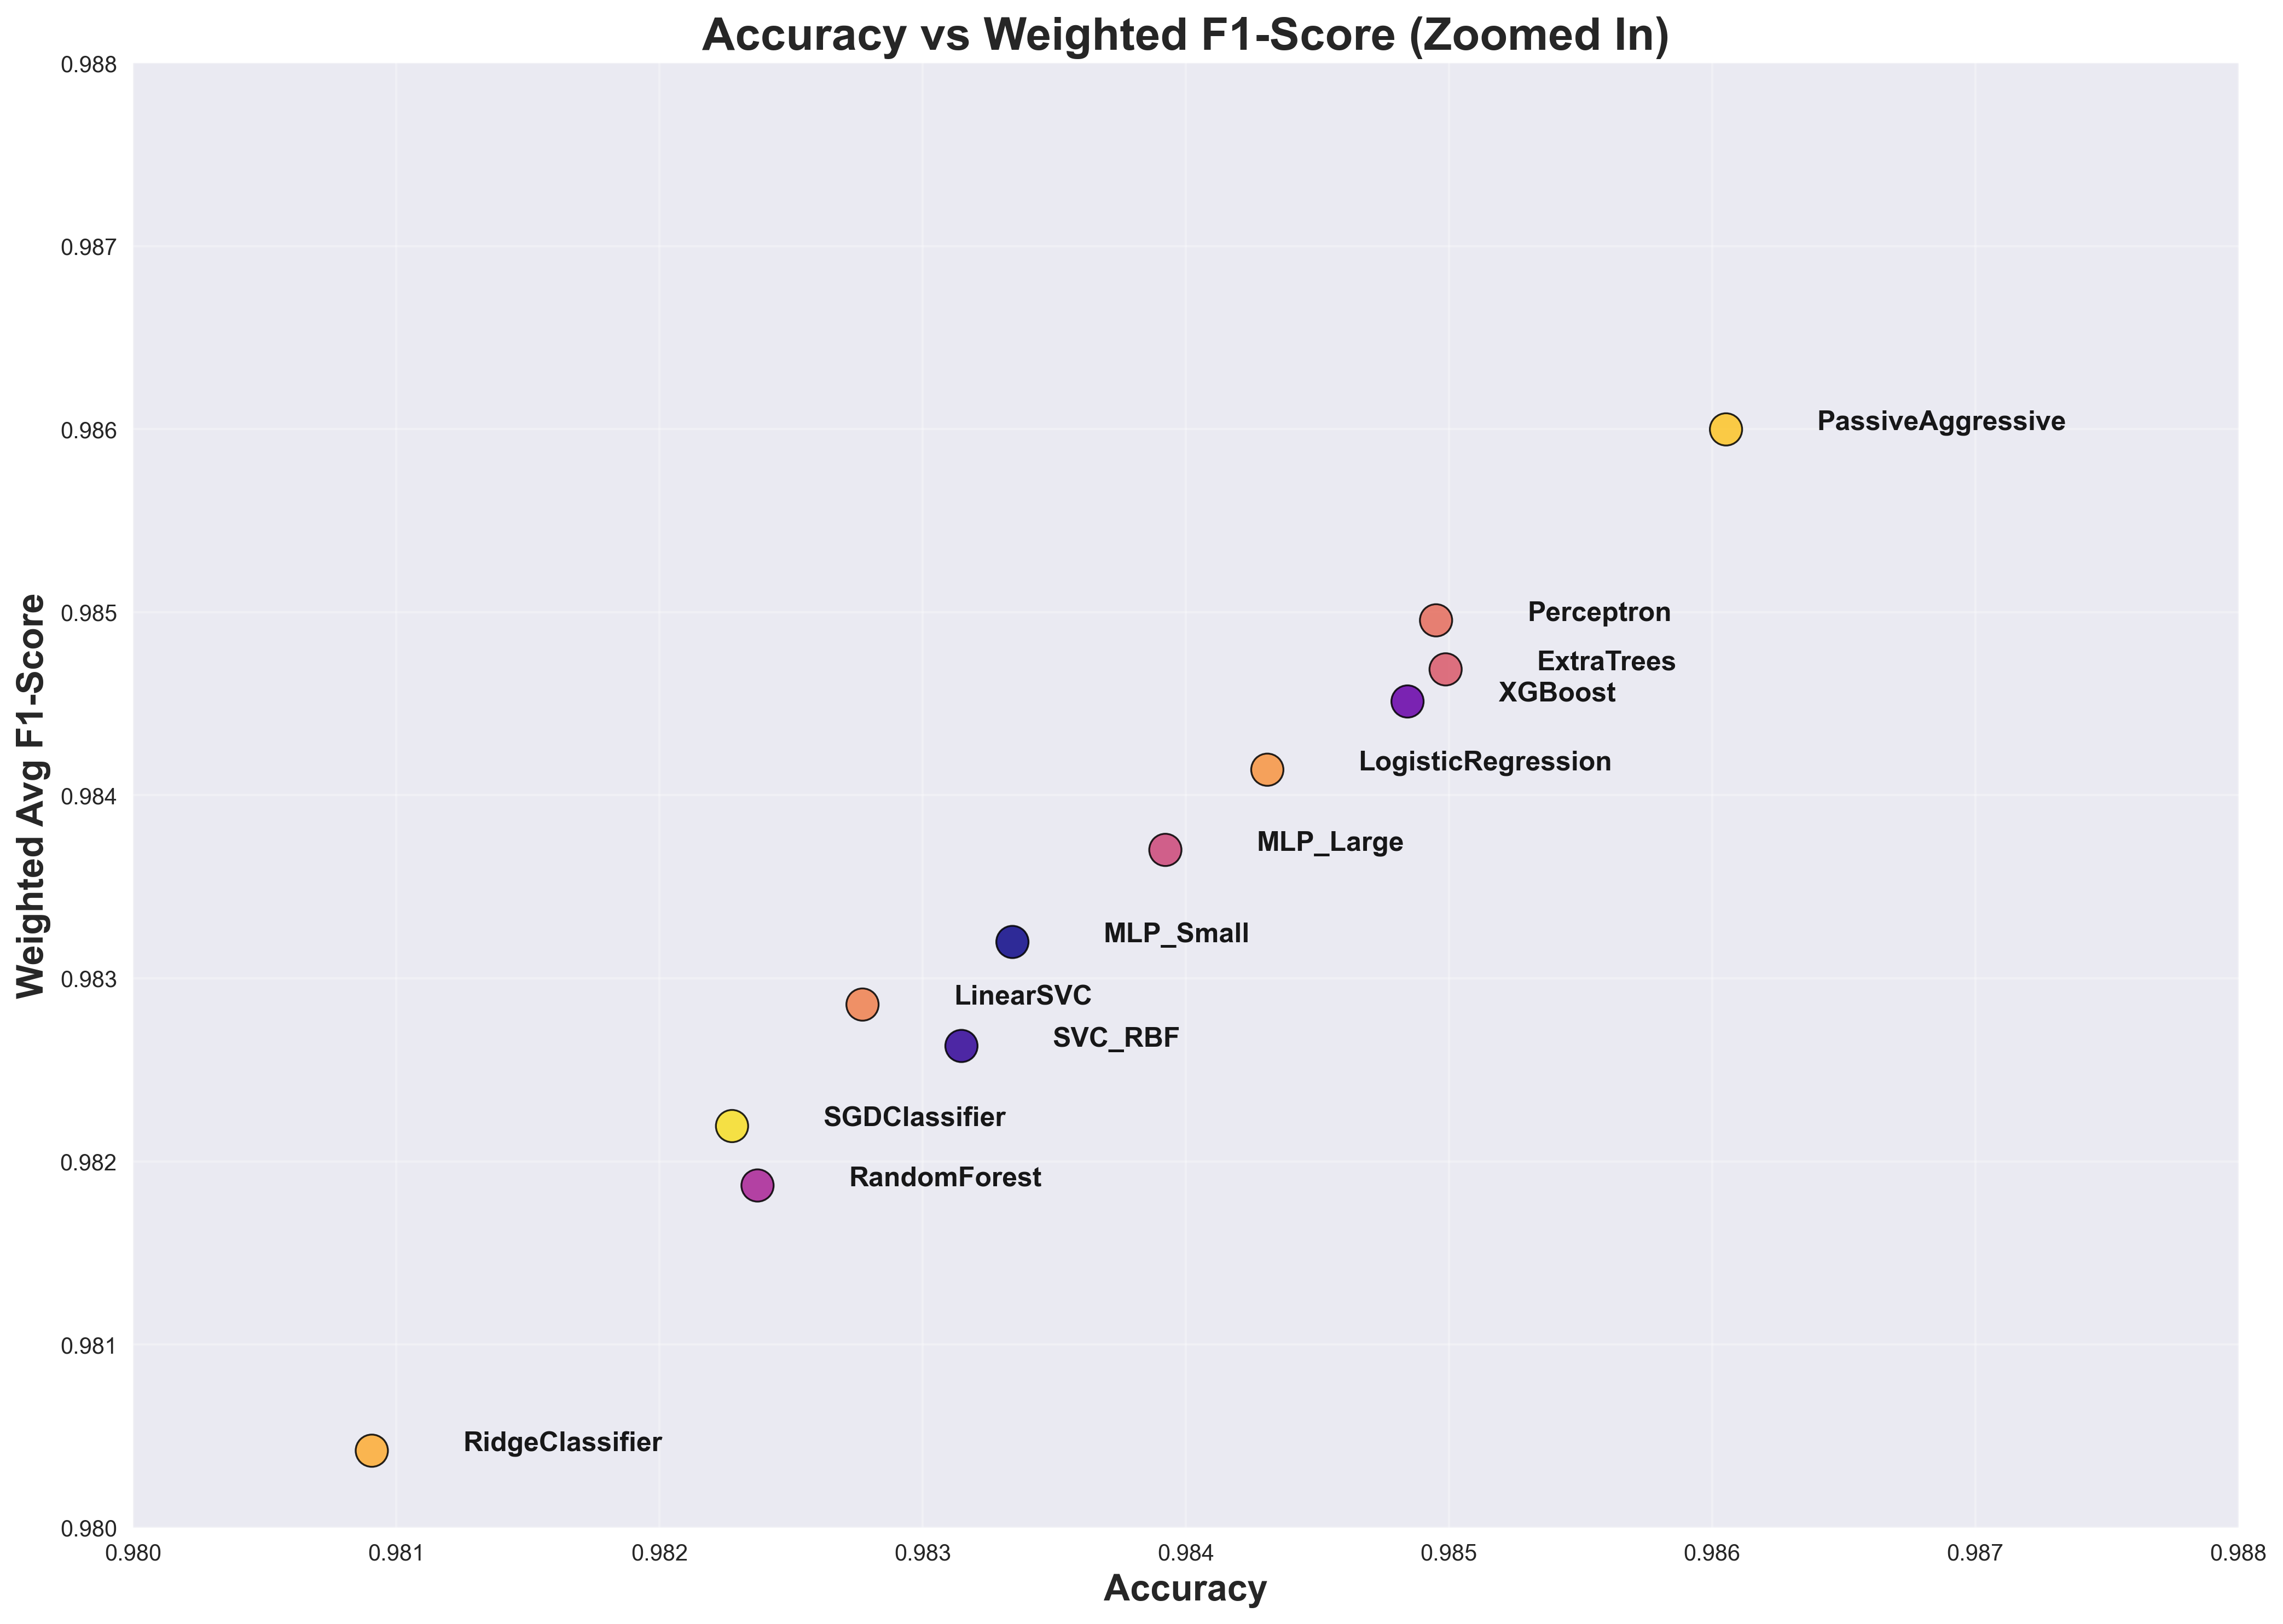
\includegraphics[keepaspectratio]{figures/11_accuracy_vs_weighted_f1_zoomed.png}}

}

\caption{Scatterplot of best performing models (accuracy) vs weighted
F1-Score.}

\end{figure}%

\begin{figure}[H]

{\centering \pandocbounded{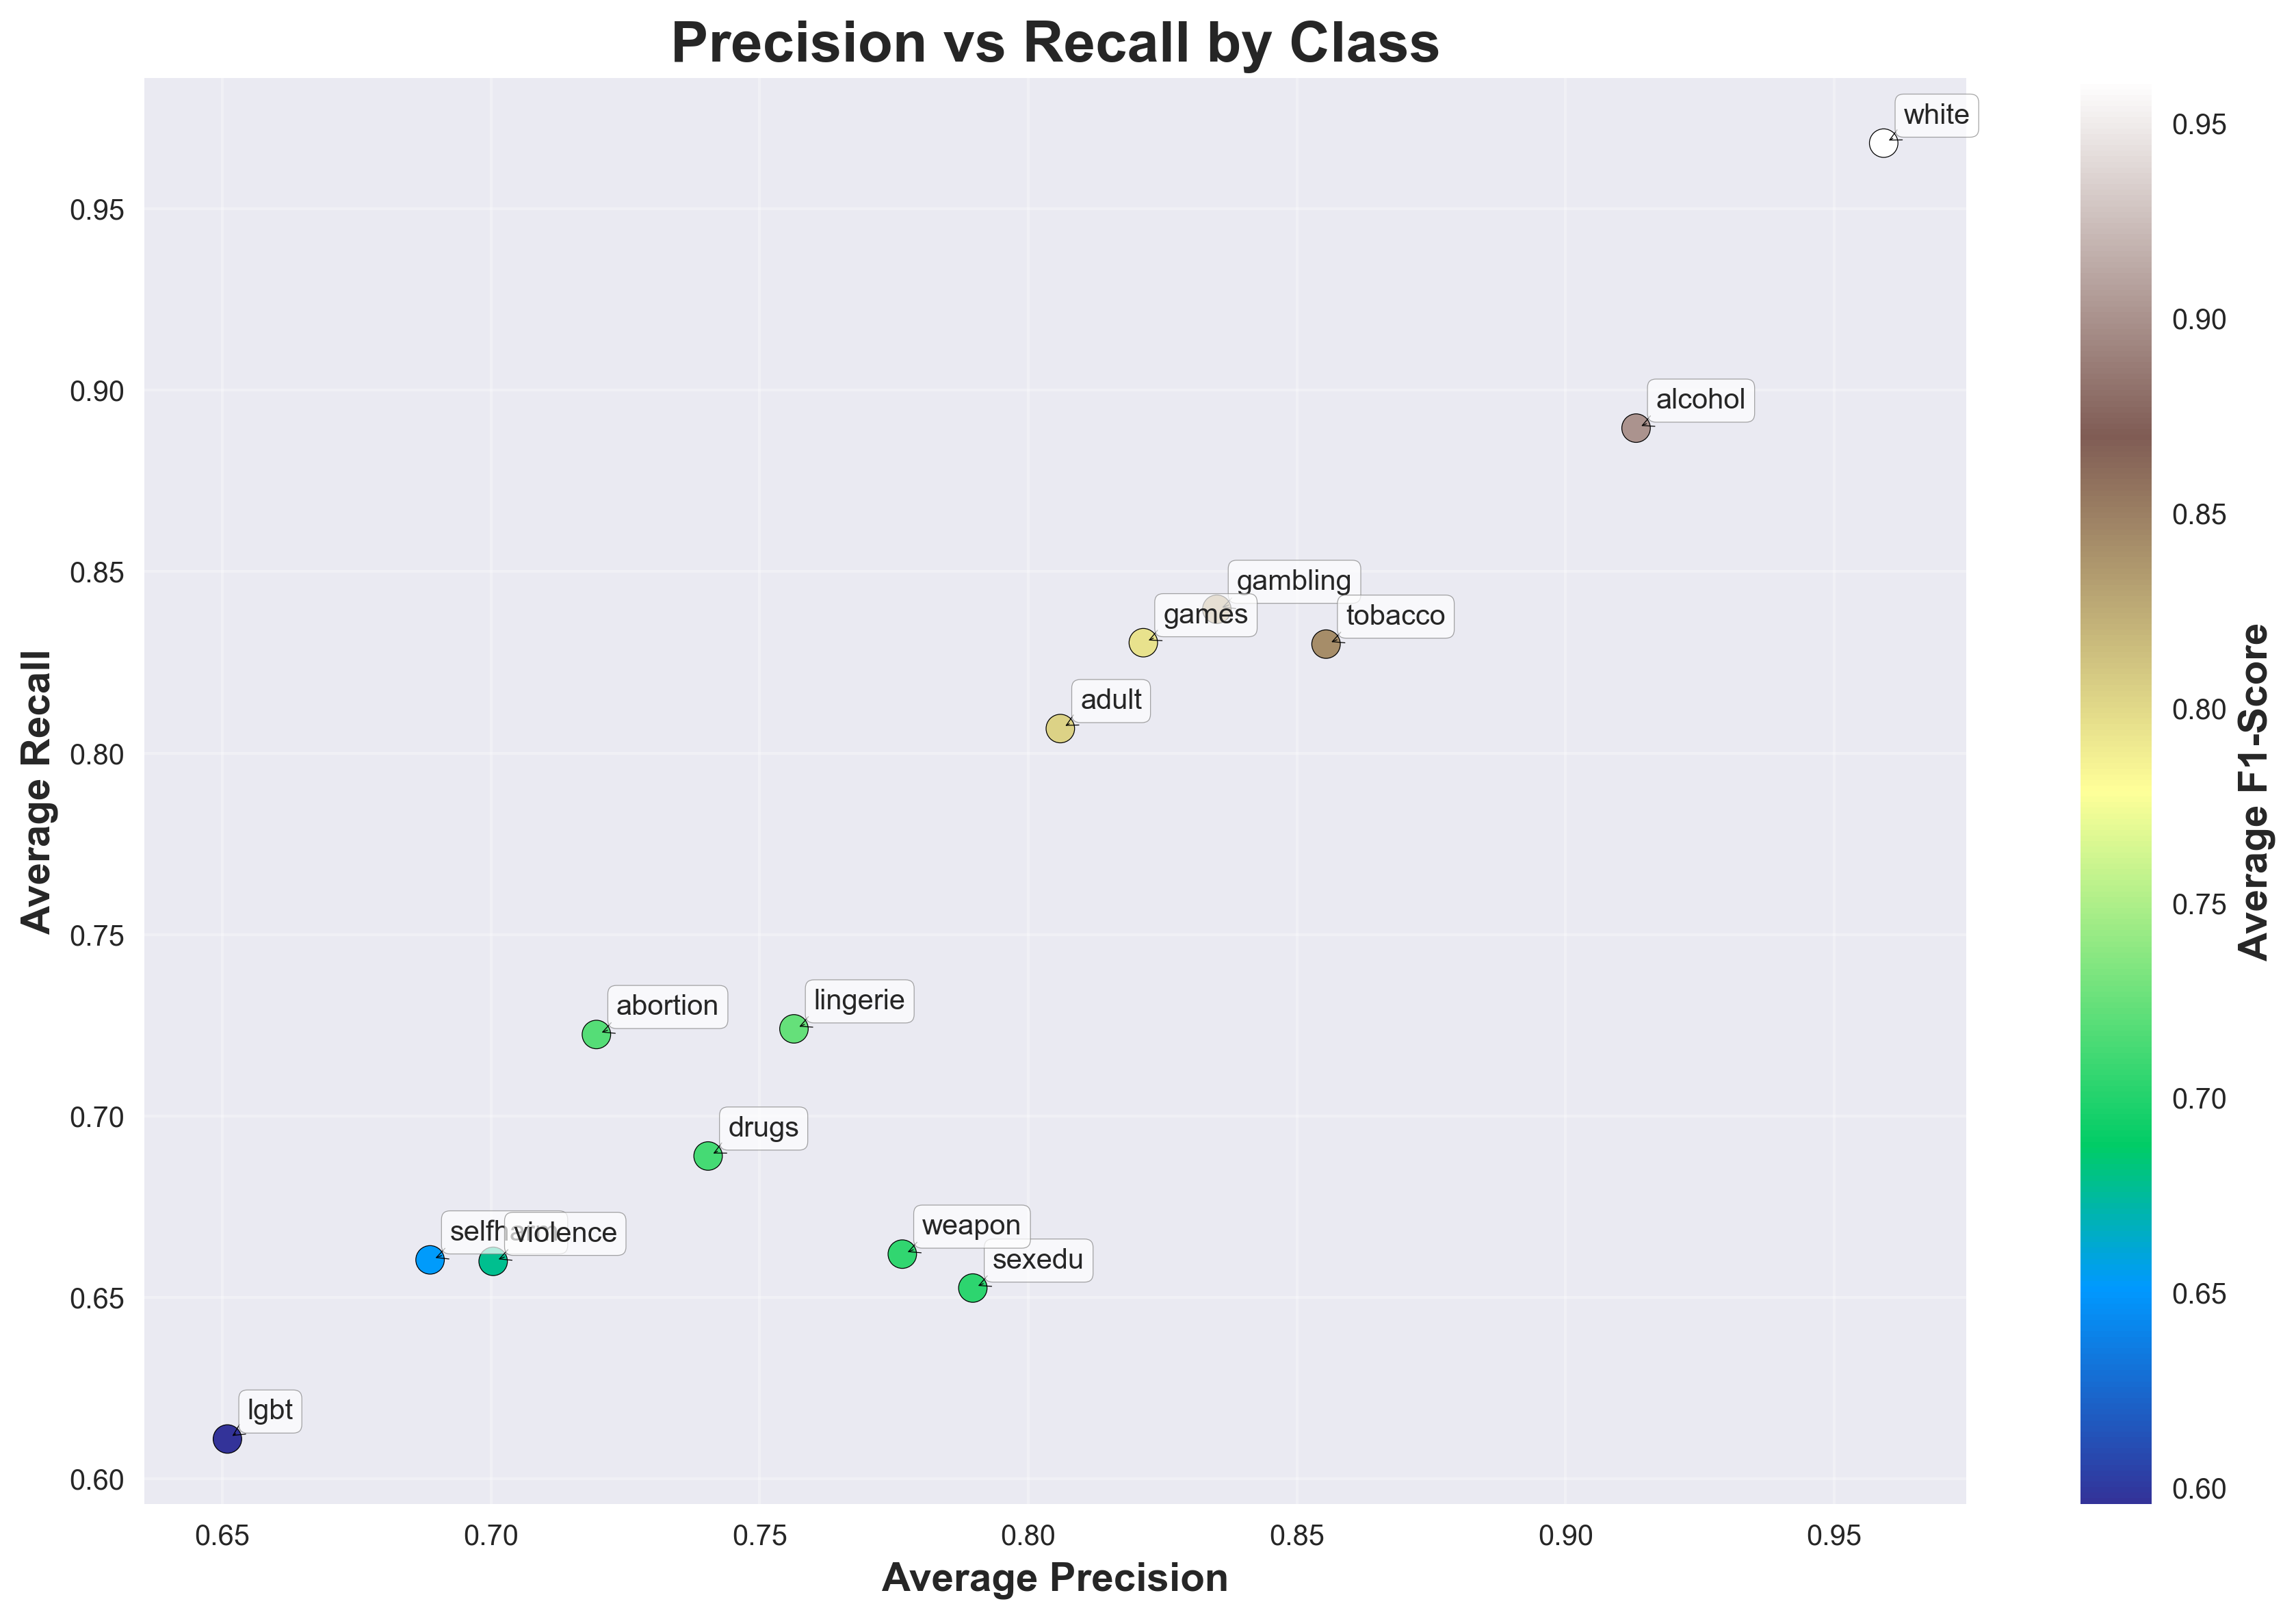
\includegraphics[keepaspectratio]{figures/12_precision_vs_recall.png}}

}

\caption{Macro-averaged precision vs recall of all data categories.}

\end{figure}%

\begin{longtable}[]{@{}lllll@{}}
\caption{F1 score statistics for each class, showing mean, standard
deviation, maximum, and support.}\tabularnewline
\toprule\noalign{}
Class Name & F1 Score Mean & F1 Score Std & F1 Score Max & Support \\
\midrule\noalign{}
\endfirsthead
\toprule\noalign{}
Class Name & F1 Score Mean & F1 Score Std & F1 Score Max & Support \\
\midrule\noalign{}
\endhead
\bottomrule\noalign{}
\endlastfoot
abortion & 0.718 & 0.279 & 0.871 & 182 \\
adult & 0.803 & 0.314 & 0.967 & 594 \\
alcohol & 0.901 & 0.269 & 0.997 & 1441 \\
drugs & 0.712 & 0.278 & 0.871 & 247 \\
gambling & 0.836 & 0.325 & 0.990 & 477 \\
games & 0.795 & 0.329 & 0.986 & 702 \\
lgbt & 0.596 & 0.290 & 0.834 & 107 \\
lingerie & 0.724 & 0.316 & 0.938 & 85 \\
selfharm & 0.652 & 0.300 & 0.903 & 81 \\
sexedu & 0.704 & 0.284 & 0.947 & 20 \\
tobacco & 0.842 & 0.325 & 0.992 & 504 \\
violence & 0.677 & 0.272 & 0.863 & 273 \\
weapon & 0.706 & 0.281 & 0.880 & 221 \\
white & 0.962 & 0.064 & 0.997 & 15716 \\
\end{longtable}

At the same time, it is worth noting that some categories are relatively
easier to classify compared to other models. For example, categories
such as alcohol, adult, and gambling, all have a relatively high
F1-Macro score while classes such as violence, lgbt, and selfharm all
perform rather poorly in terms of model performance. The precision vs
recall metrics reveal more about the classes themselves, highlighting
the difficulty models have with classifying certain categories of the
data, highlighting the need for further fine-tuning.

\begin{figure}[H]

{\centering \pandocbounded{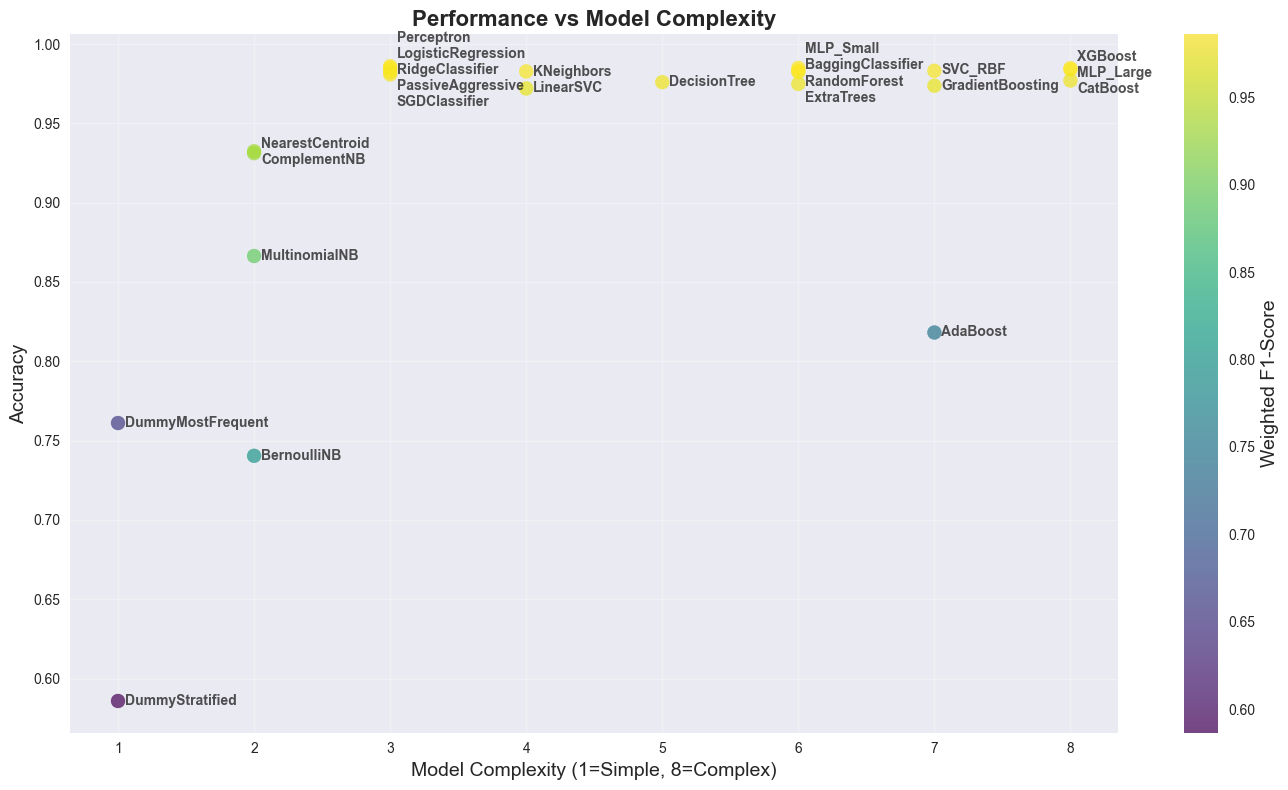
\includegraphics[keepaspectratio]{figures/13_complexity_vs_performance.png}}

}

\caption{Model complexity vs performance.}

\end{figure}%

It is also worth noting that more complex models perform better when
compared to simple models, yet that statement fails to hold beyond
moderately complex models.

\begin{figure}[H]

{\centering \pandocbounded{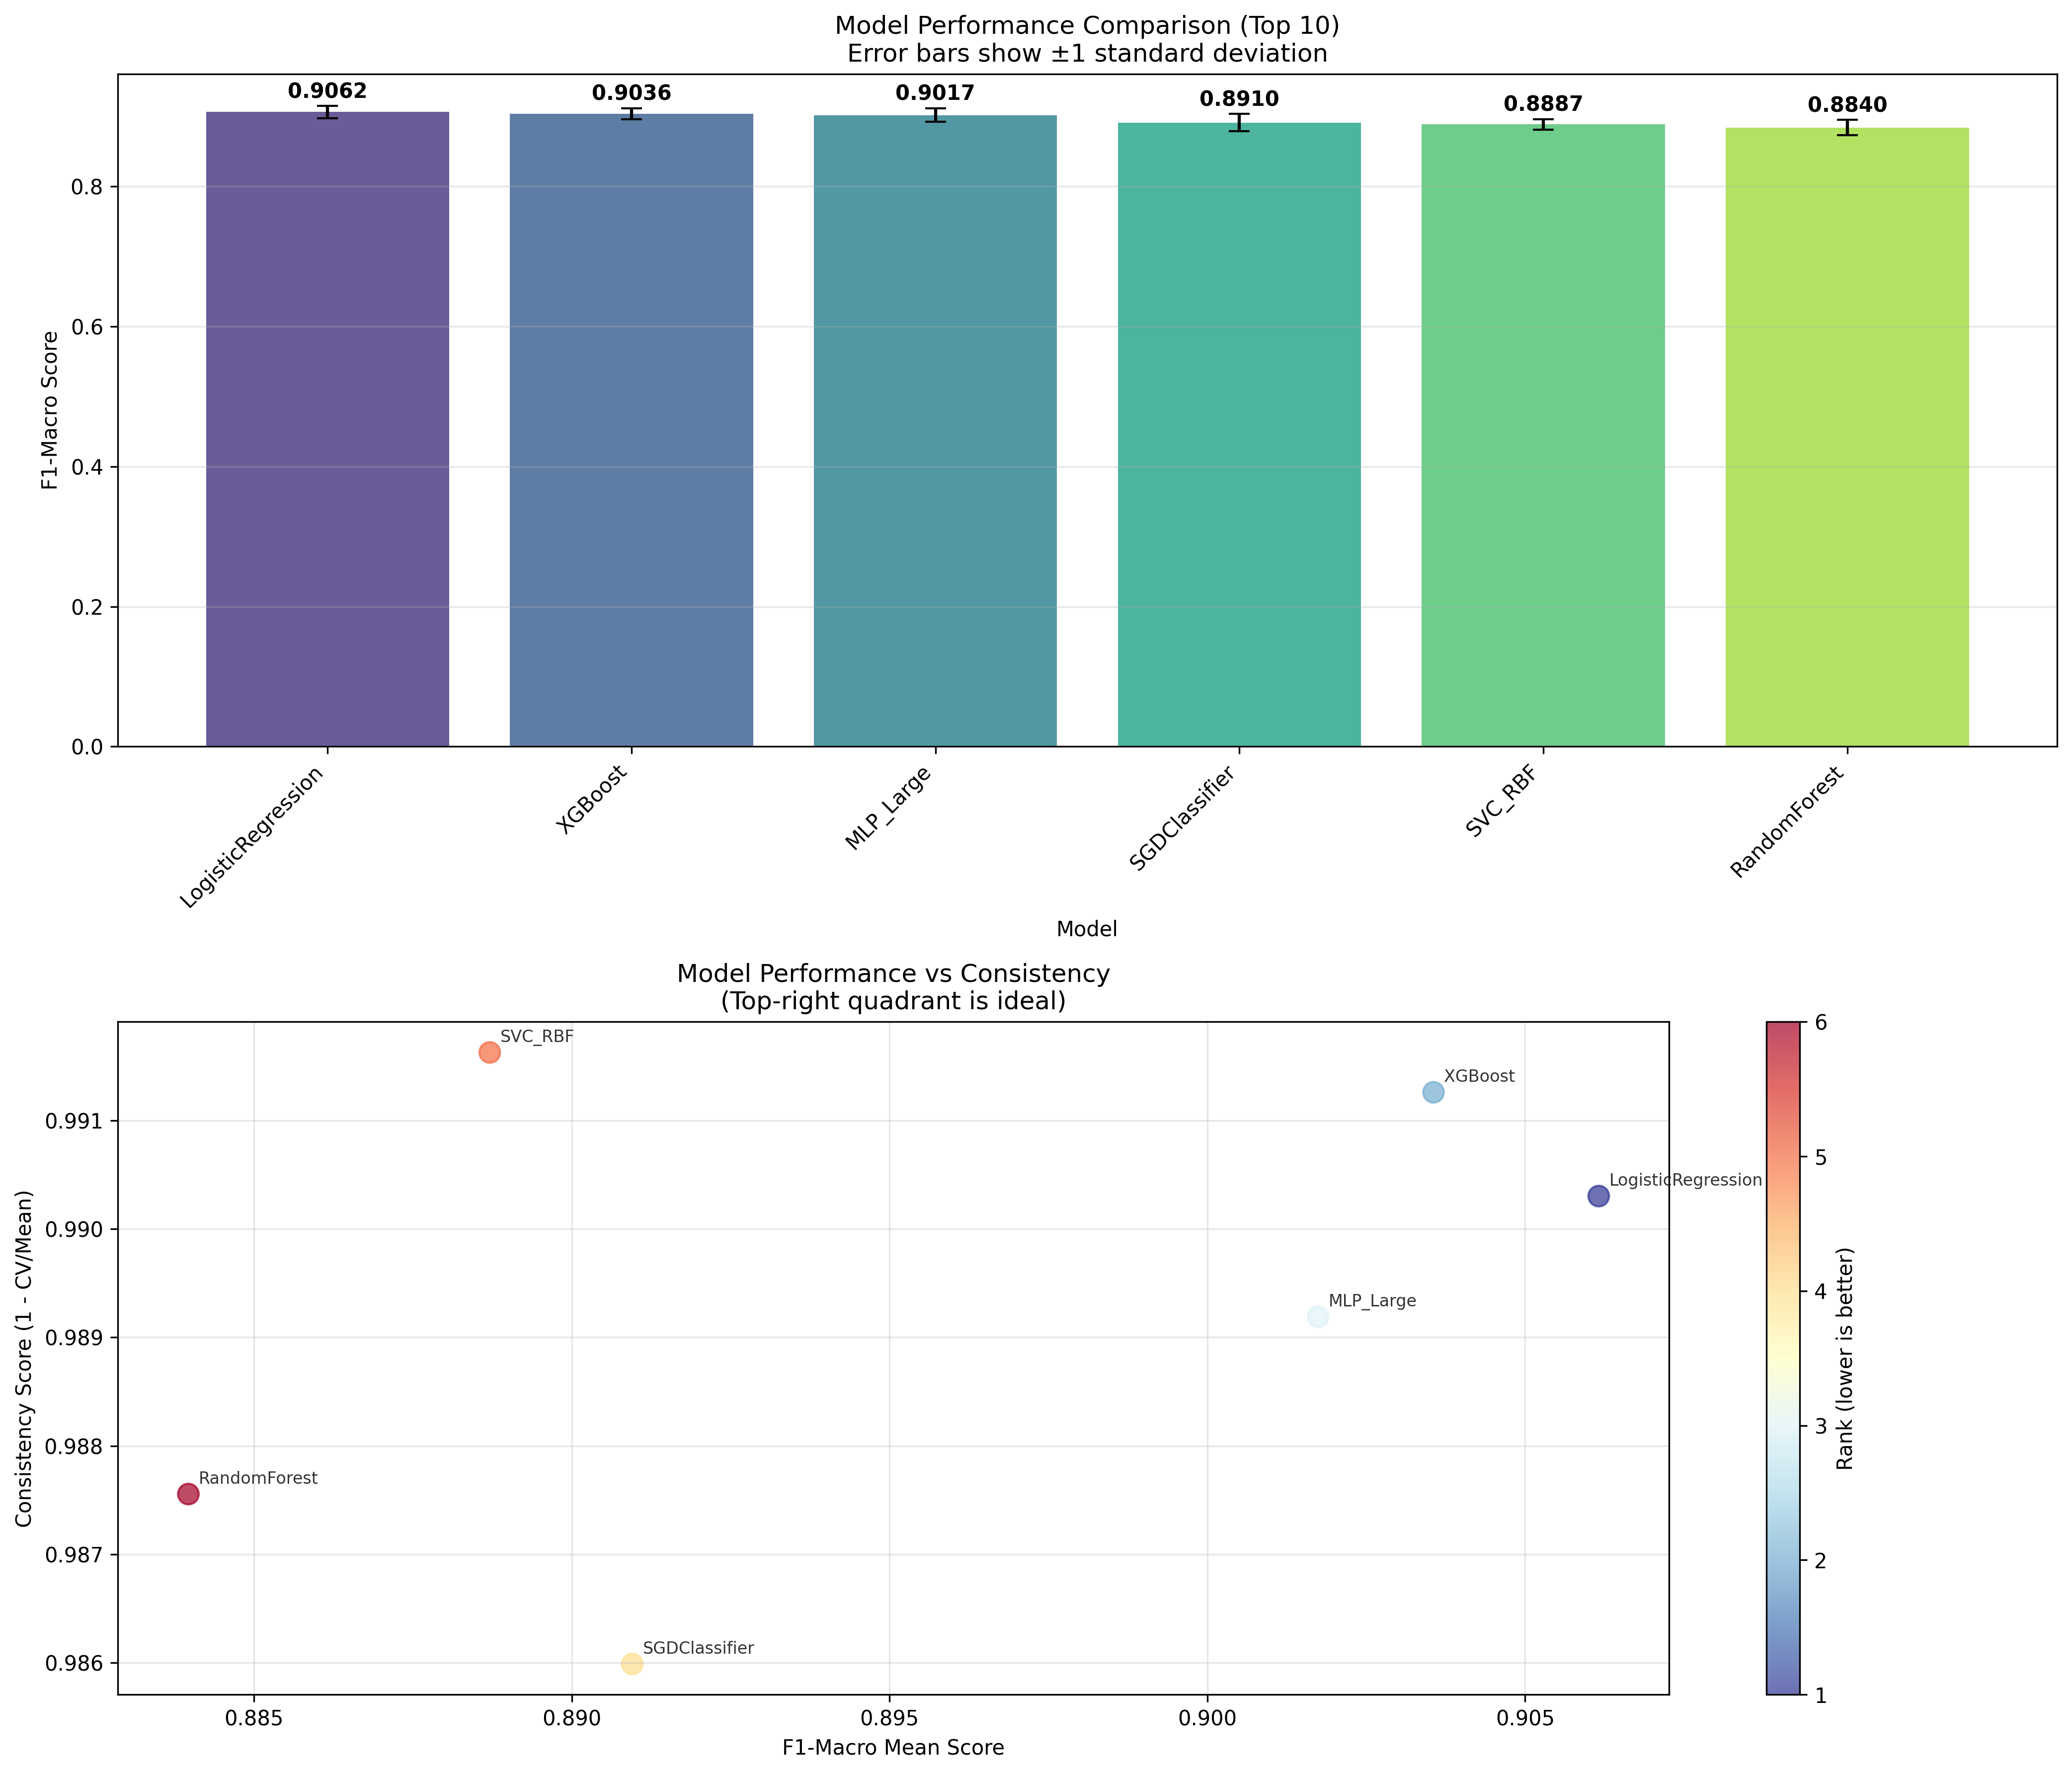
\includegraphics[keepaspectratio]{figures/15_v4.6.5_six_model.png}}

}

\caption{Top: Model performance along with average performance
evaluation. Bottom: Model rank and consistency.}

\end{figure}%

\begin{figure}[H]

{\centering \pandocbounded{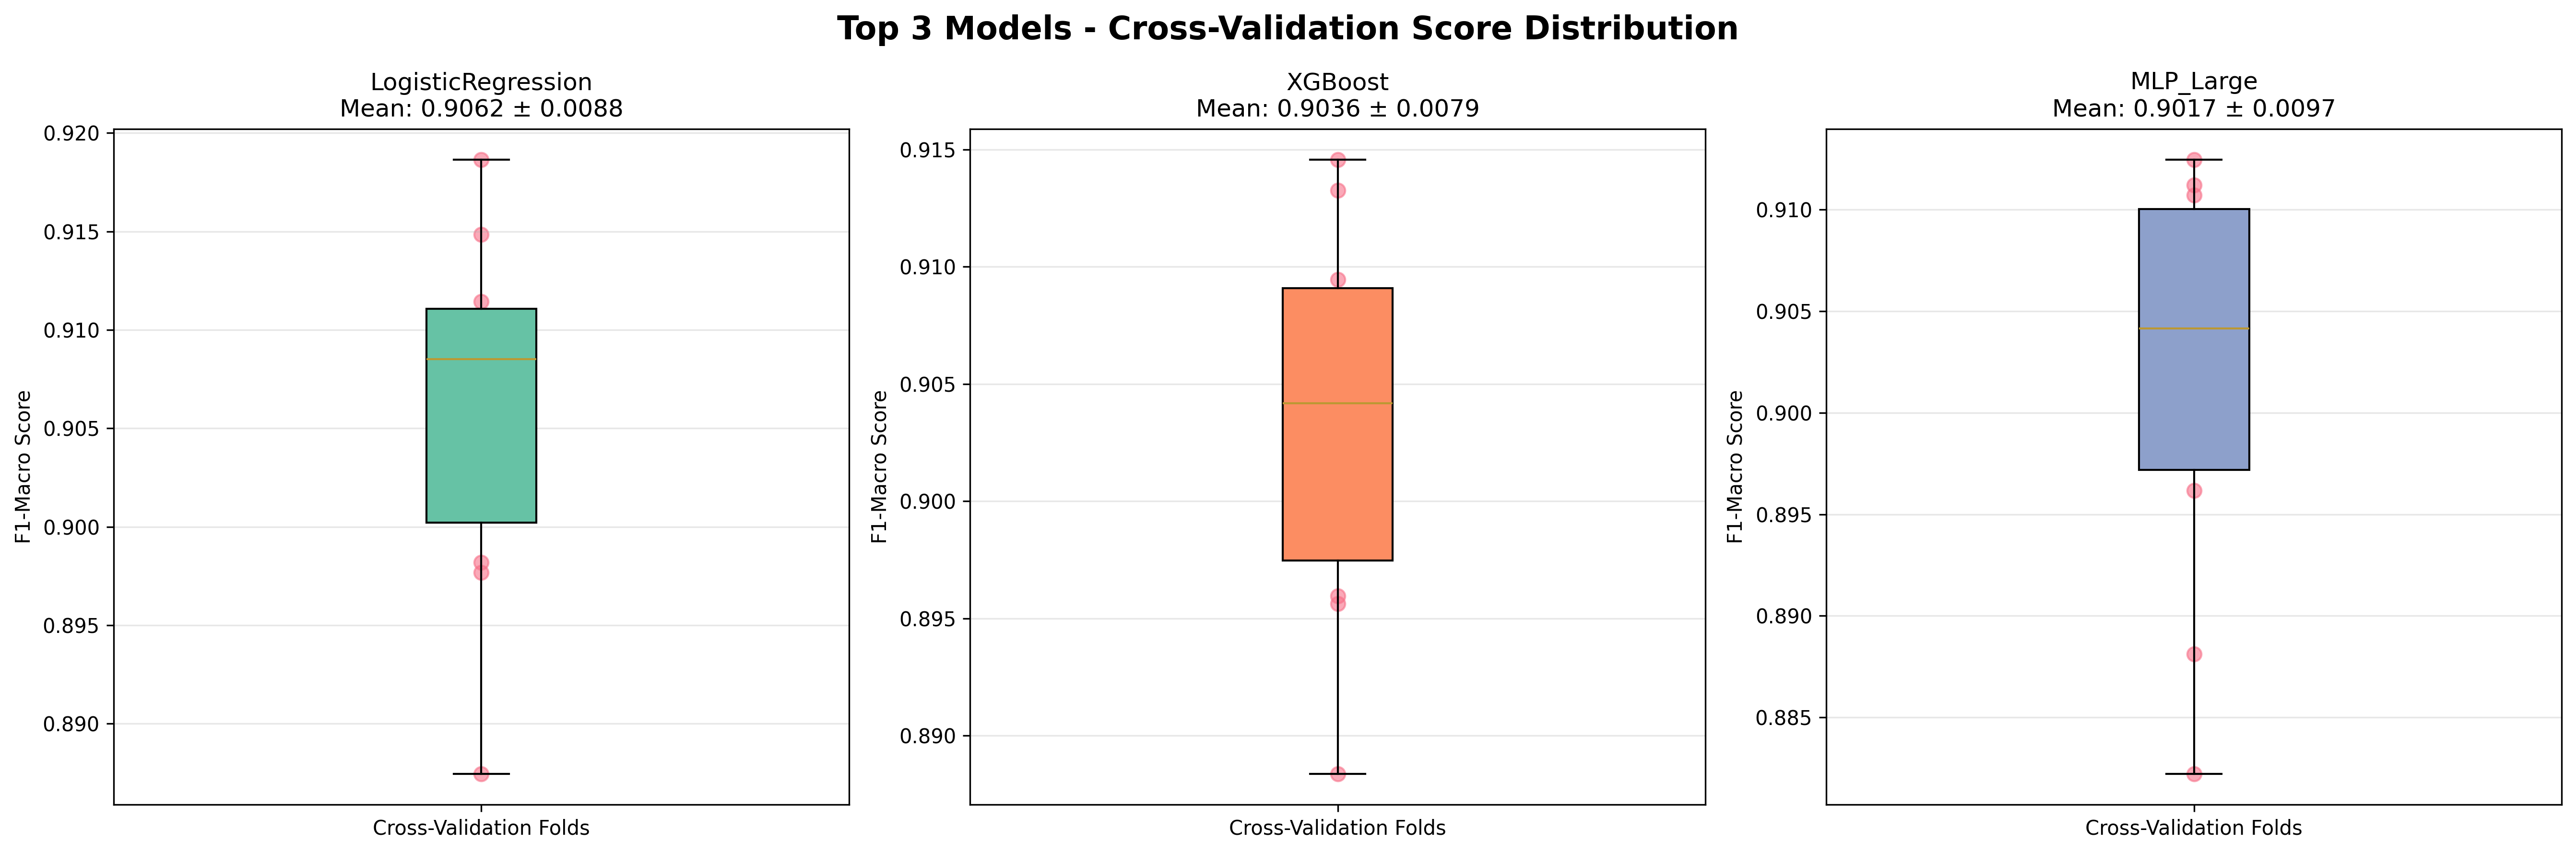
\includegraphics[keepaspectratio]{figures/16_v4.6.5_three_model.png}}

}

\caption{Cross Validation distribution across the top 3 models after
initial default search.}

\end{figure}%

Six of the best models were selected and compared across 10-fold CV,
with the top 3 models consistently achieving a mean F1-Macro score of
around 0.9. As a result, boosted trees, logistic regression, and
LinearSVC were selected for the purpose of further fine tuning.

\subsection{Boosted Trees}\label{boosted-trees-1}

\subsubsection{LightGBM}\label{lightgbm-1}

\begin{figure}[H]

{\centering \pandocbounded{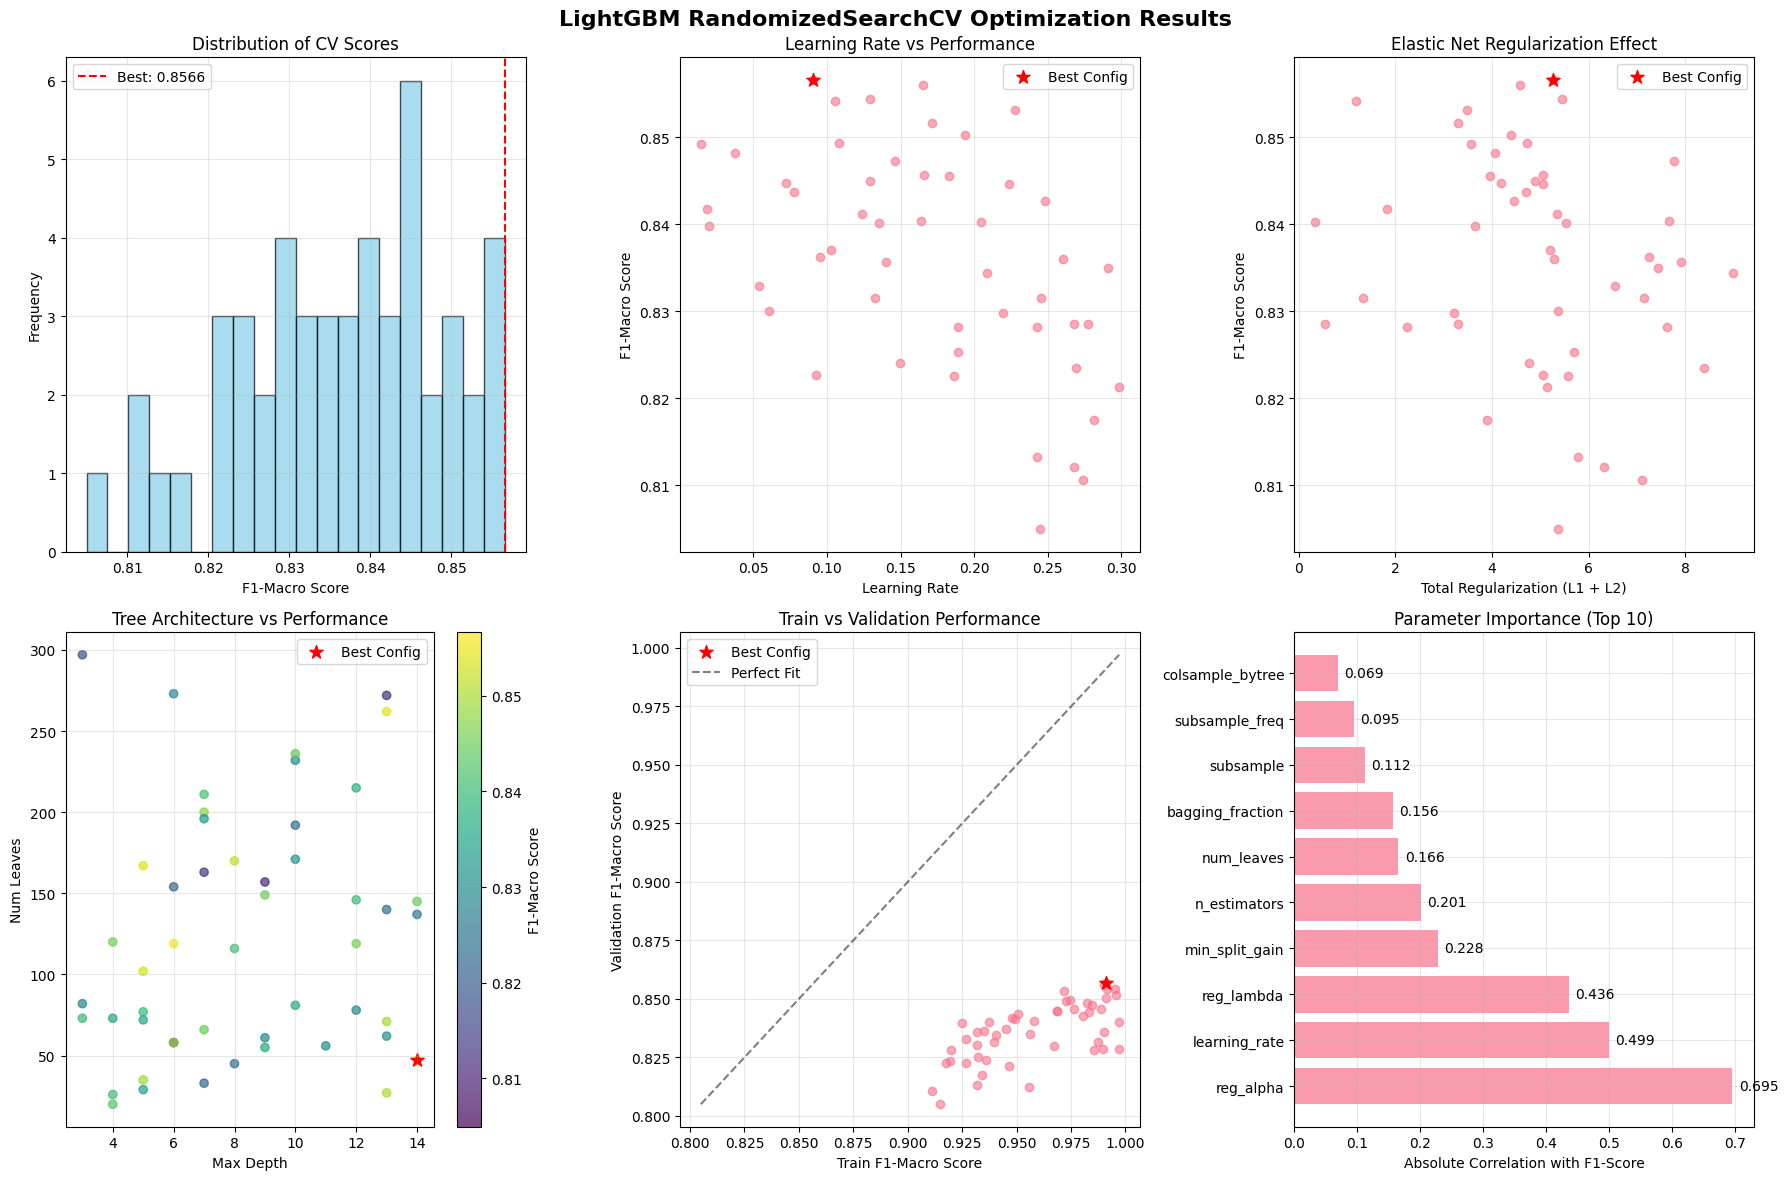
\includegraphics[keepaspectratio]{figures/17_v4.5.1_lgbm_search.png}}

}

\caption{LightGBM randomized hyperparameter search results.}

\end{figure}%

The results from a simple hyperparameter search with 40 iterations of
LightGBM revealed that the best validation Macro-Averaged F1-score would
still show significant signs of overfitting due to the steep difference
between train and validation iteration scores consistently across all
models tested. A large max-depth and a small number of leaves for each
tree also indicates that overfitting is highly likely in this setup.

\subsubsection{XGBoost}\label{xgboost-1}

\begin{figure}[H]

{\centering \pandocbounded{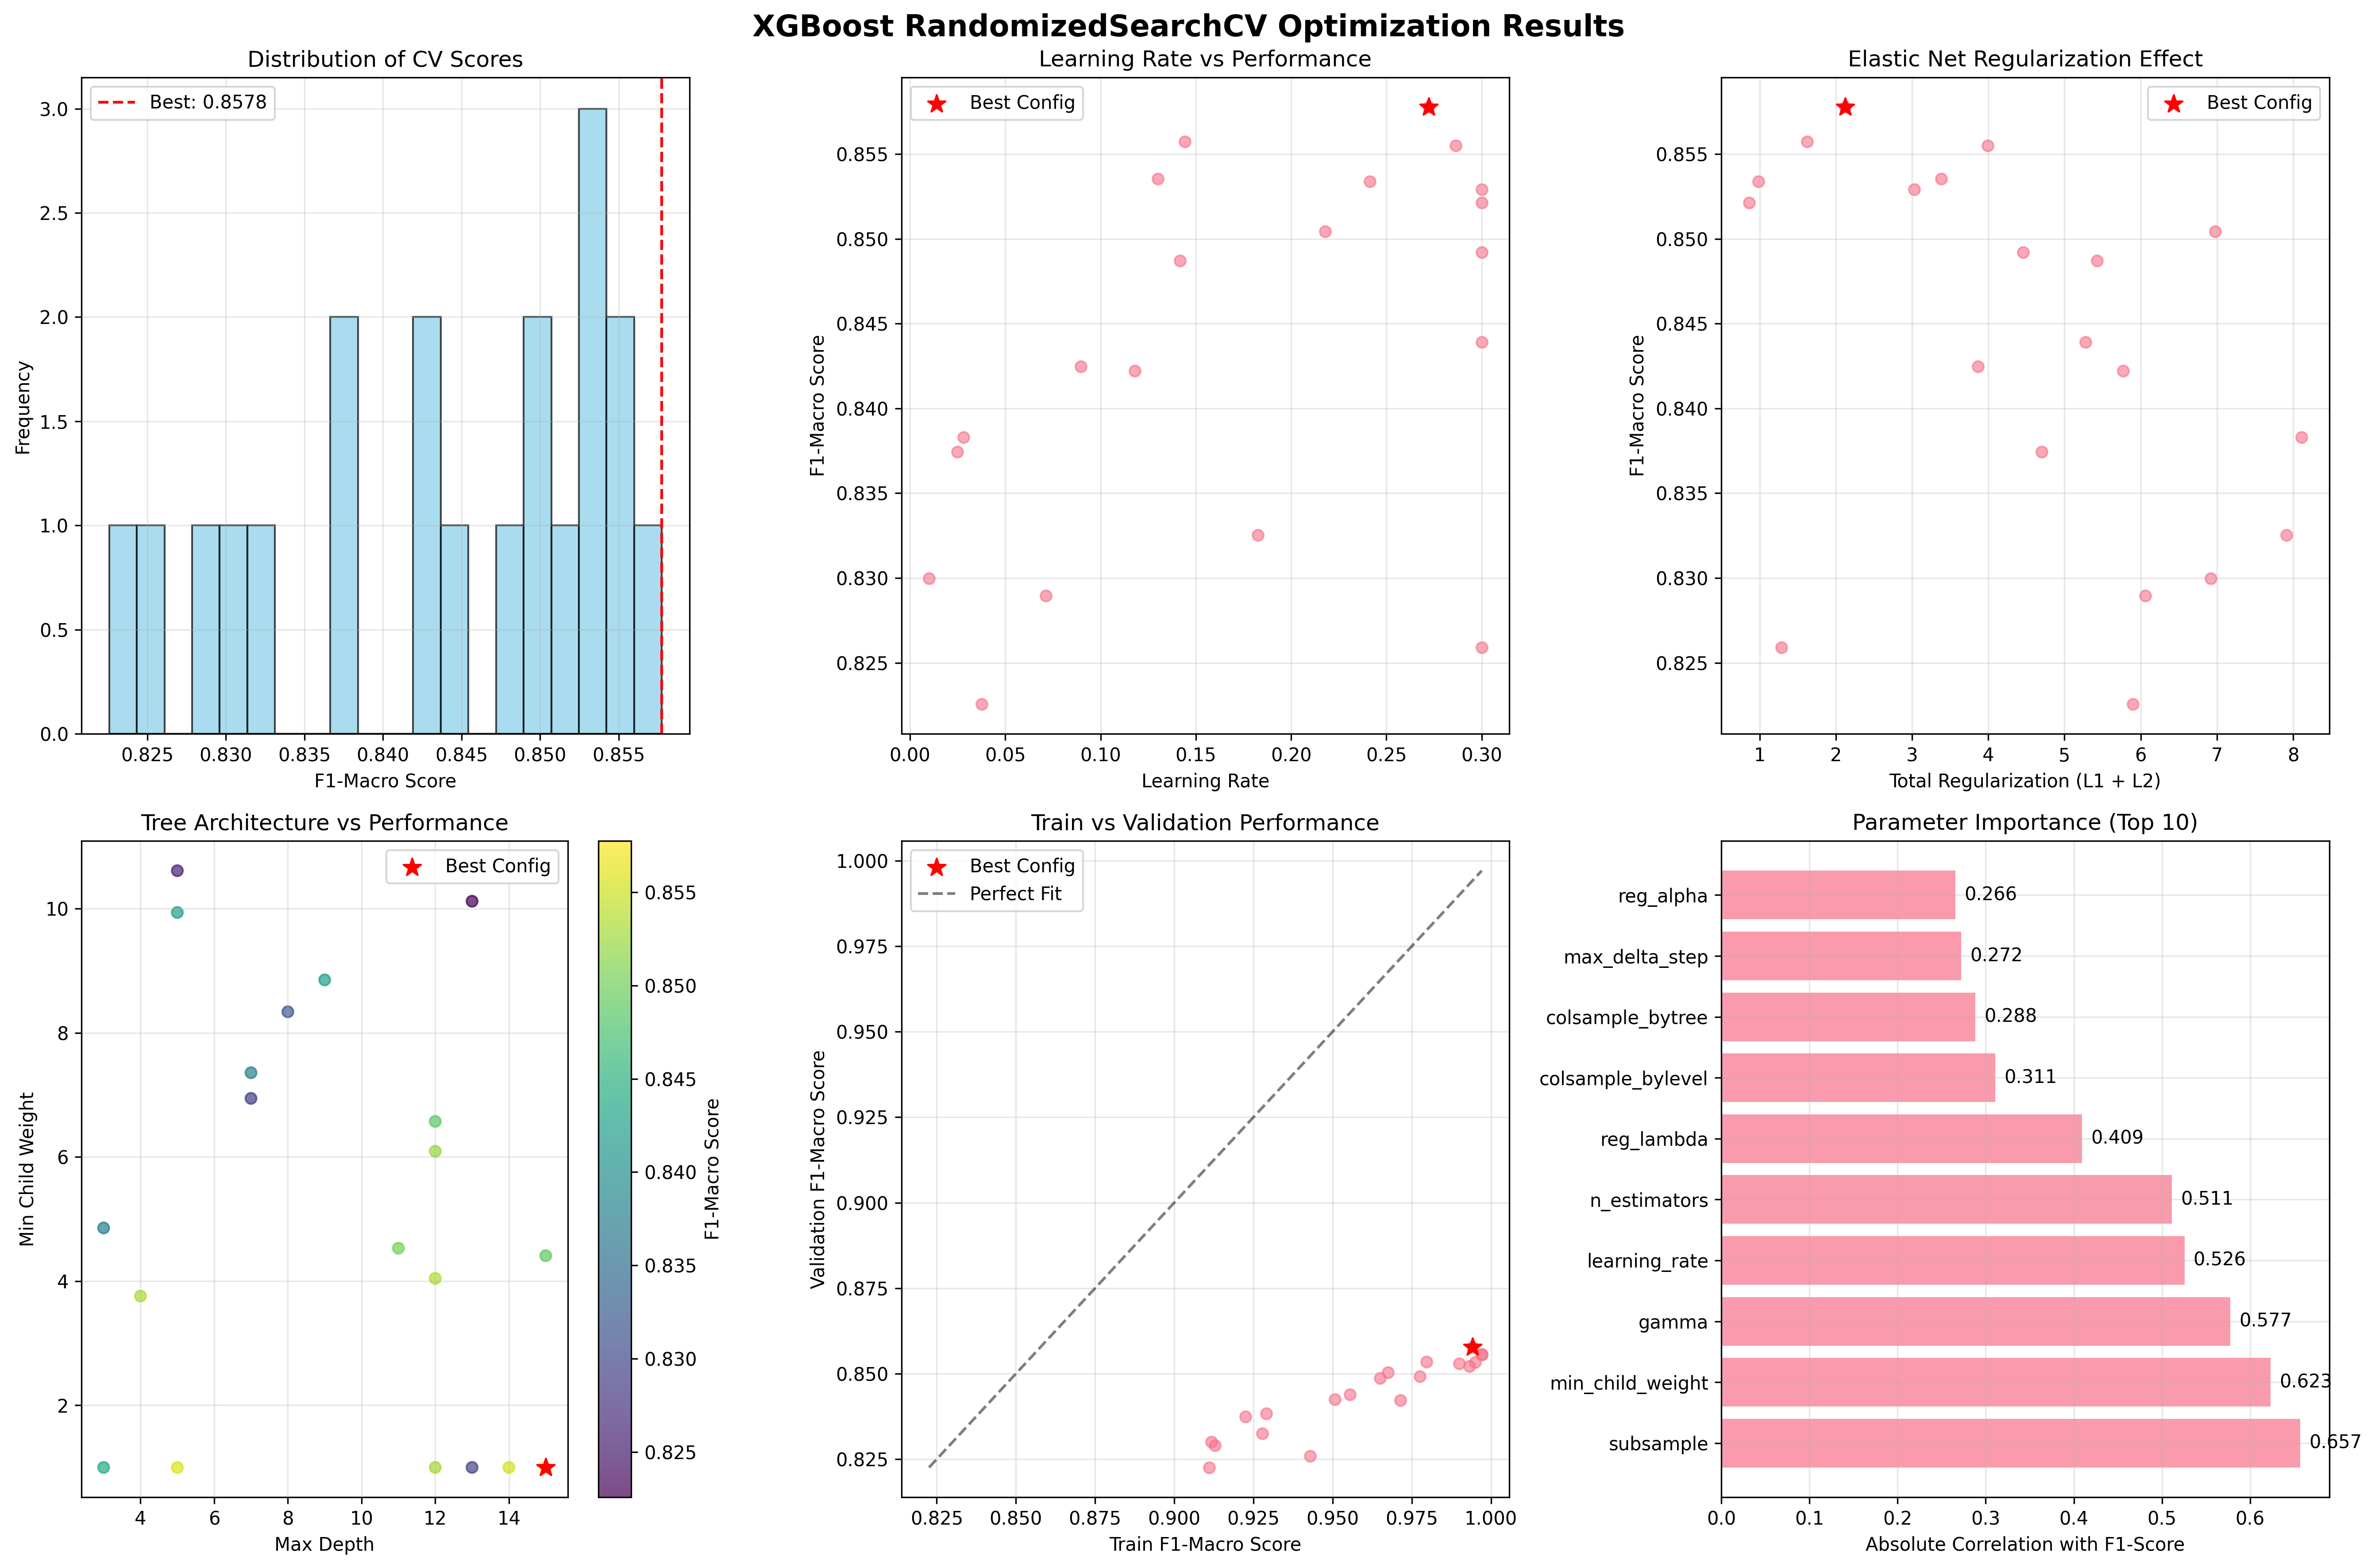
\includegraphics[keepaspectratio]{figures/18_v4.5.7_xgboost_randomized_search_results_reduced.png}}

}

\caption{XGBoost randomized hyperparameter search results.}

\end{figure}%

Similar to LightGBM, XGBoost also shows similar traits of overfitting as
evident by similar train-test F1-macro scores. However, it seems that
XGBoost is less reliant on regularization parameters and seems to
achieve better performance with less reliance on regularization
hyperparameters.

\begin{figure}[H]

{\centering \pandocbounded{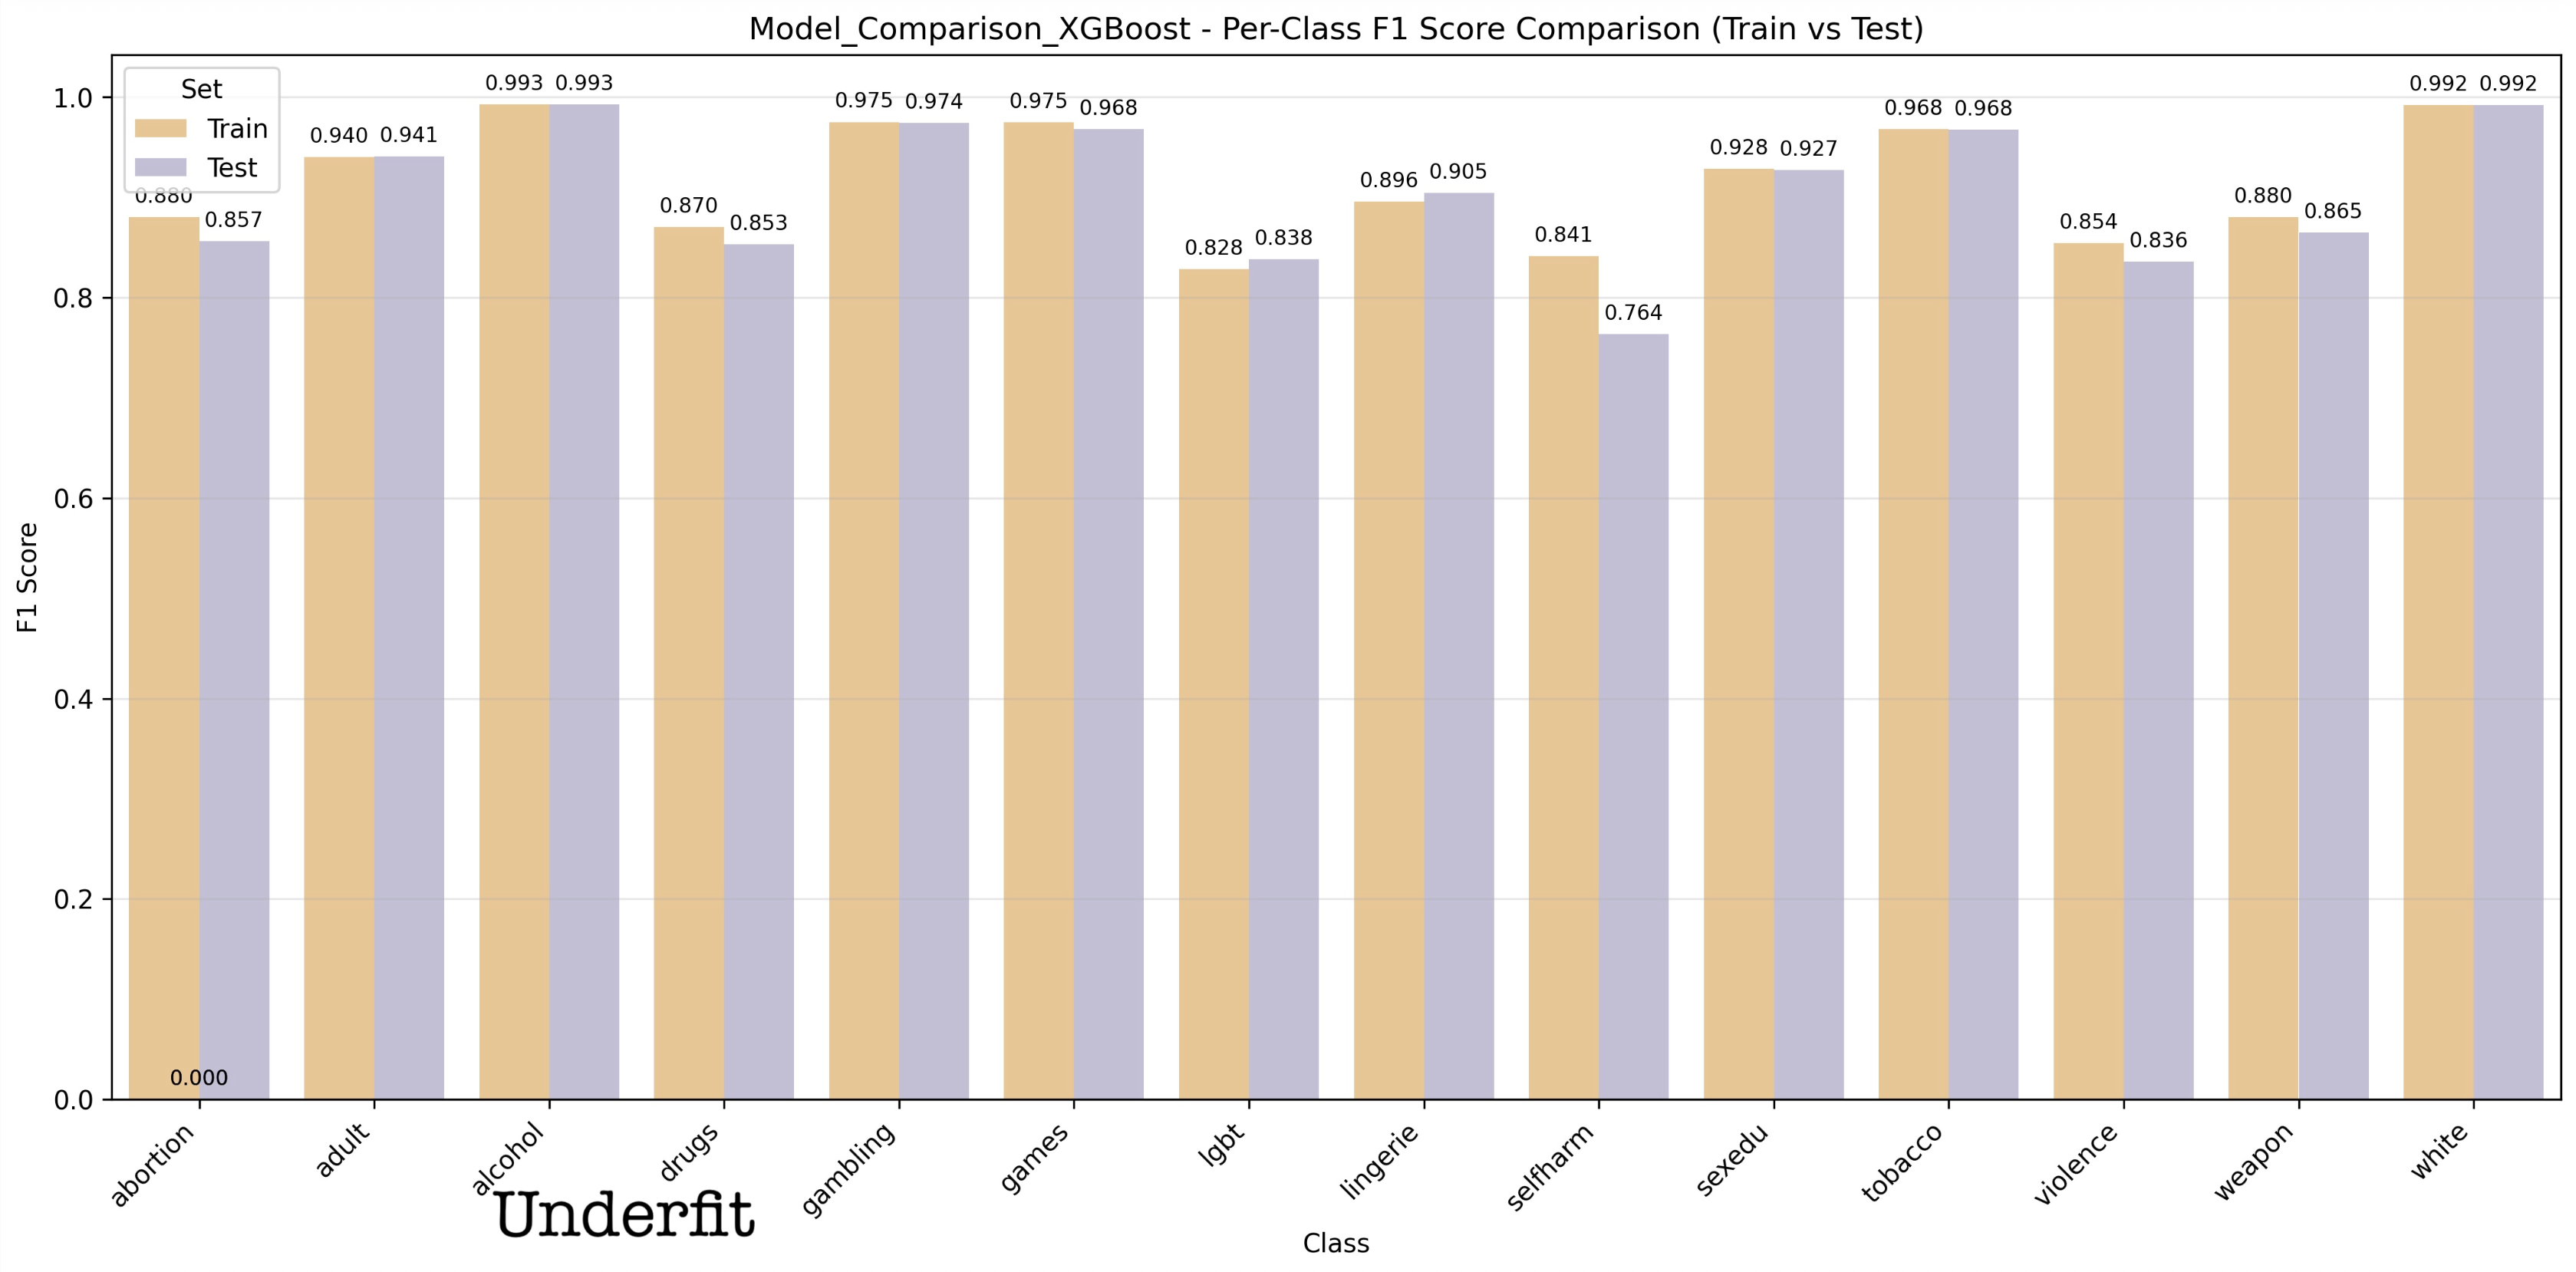
\includegraphics[keepaspectratio]{figures/19_4.5.2_xgboost_underfit.png}}

}

\caption{Underfitted model (iteration \#15) for XGBoost and train-test
F1-macro score comparison.}

\end{figure}%

During the initial exploration process for XGBoost, we can see that
there are some underfitted models that show promising results and even
signs of generalization (see lingerie category).

\begin{figure}[H]

{\centering \pandocbounded{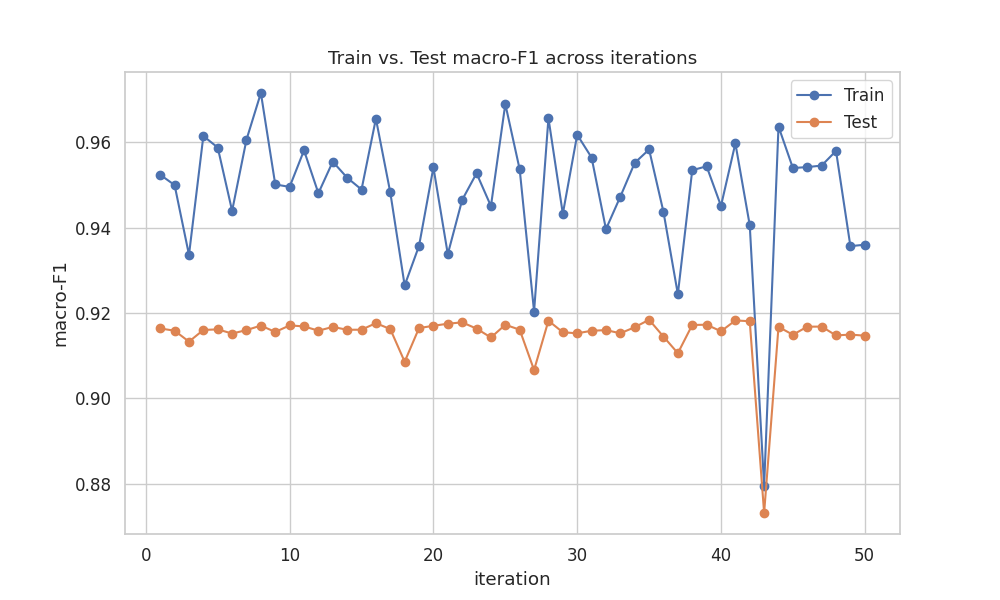
\includegraphics[keepaspectratio]{figures/20_train_test_macro_custom_weights.png}}

}

\caption{XGBoost 3rd round of training with custom weights.}

\end{figure}%

After a more in-depth search of the XGBoost model with custom weights,
more promising model candidates were discovered that perform well yet do
not show obvious signs of overfitting. Such a model was submitted as a
candidate for the final XGBoost Model.

\begin{figure}[H]

{\centering \pandocbounded{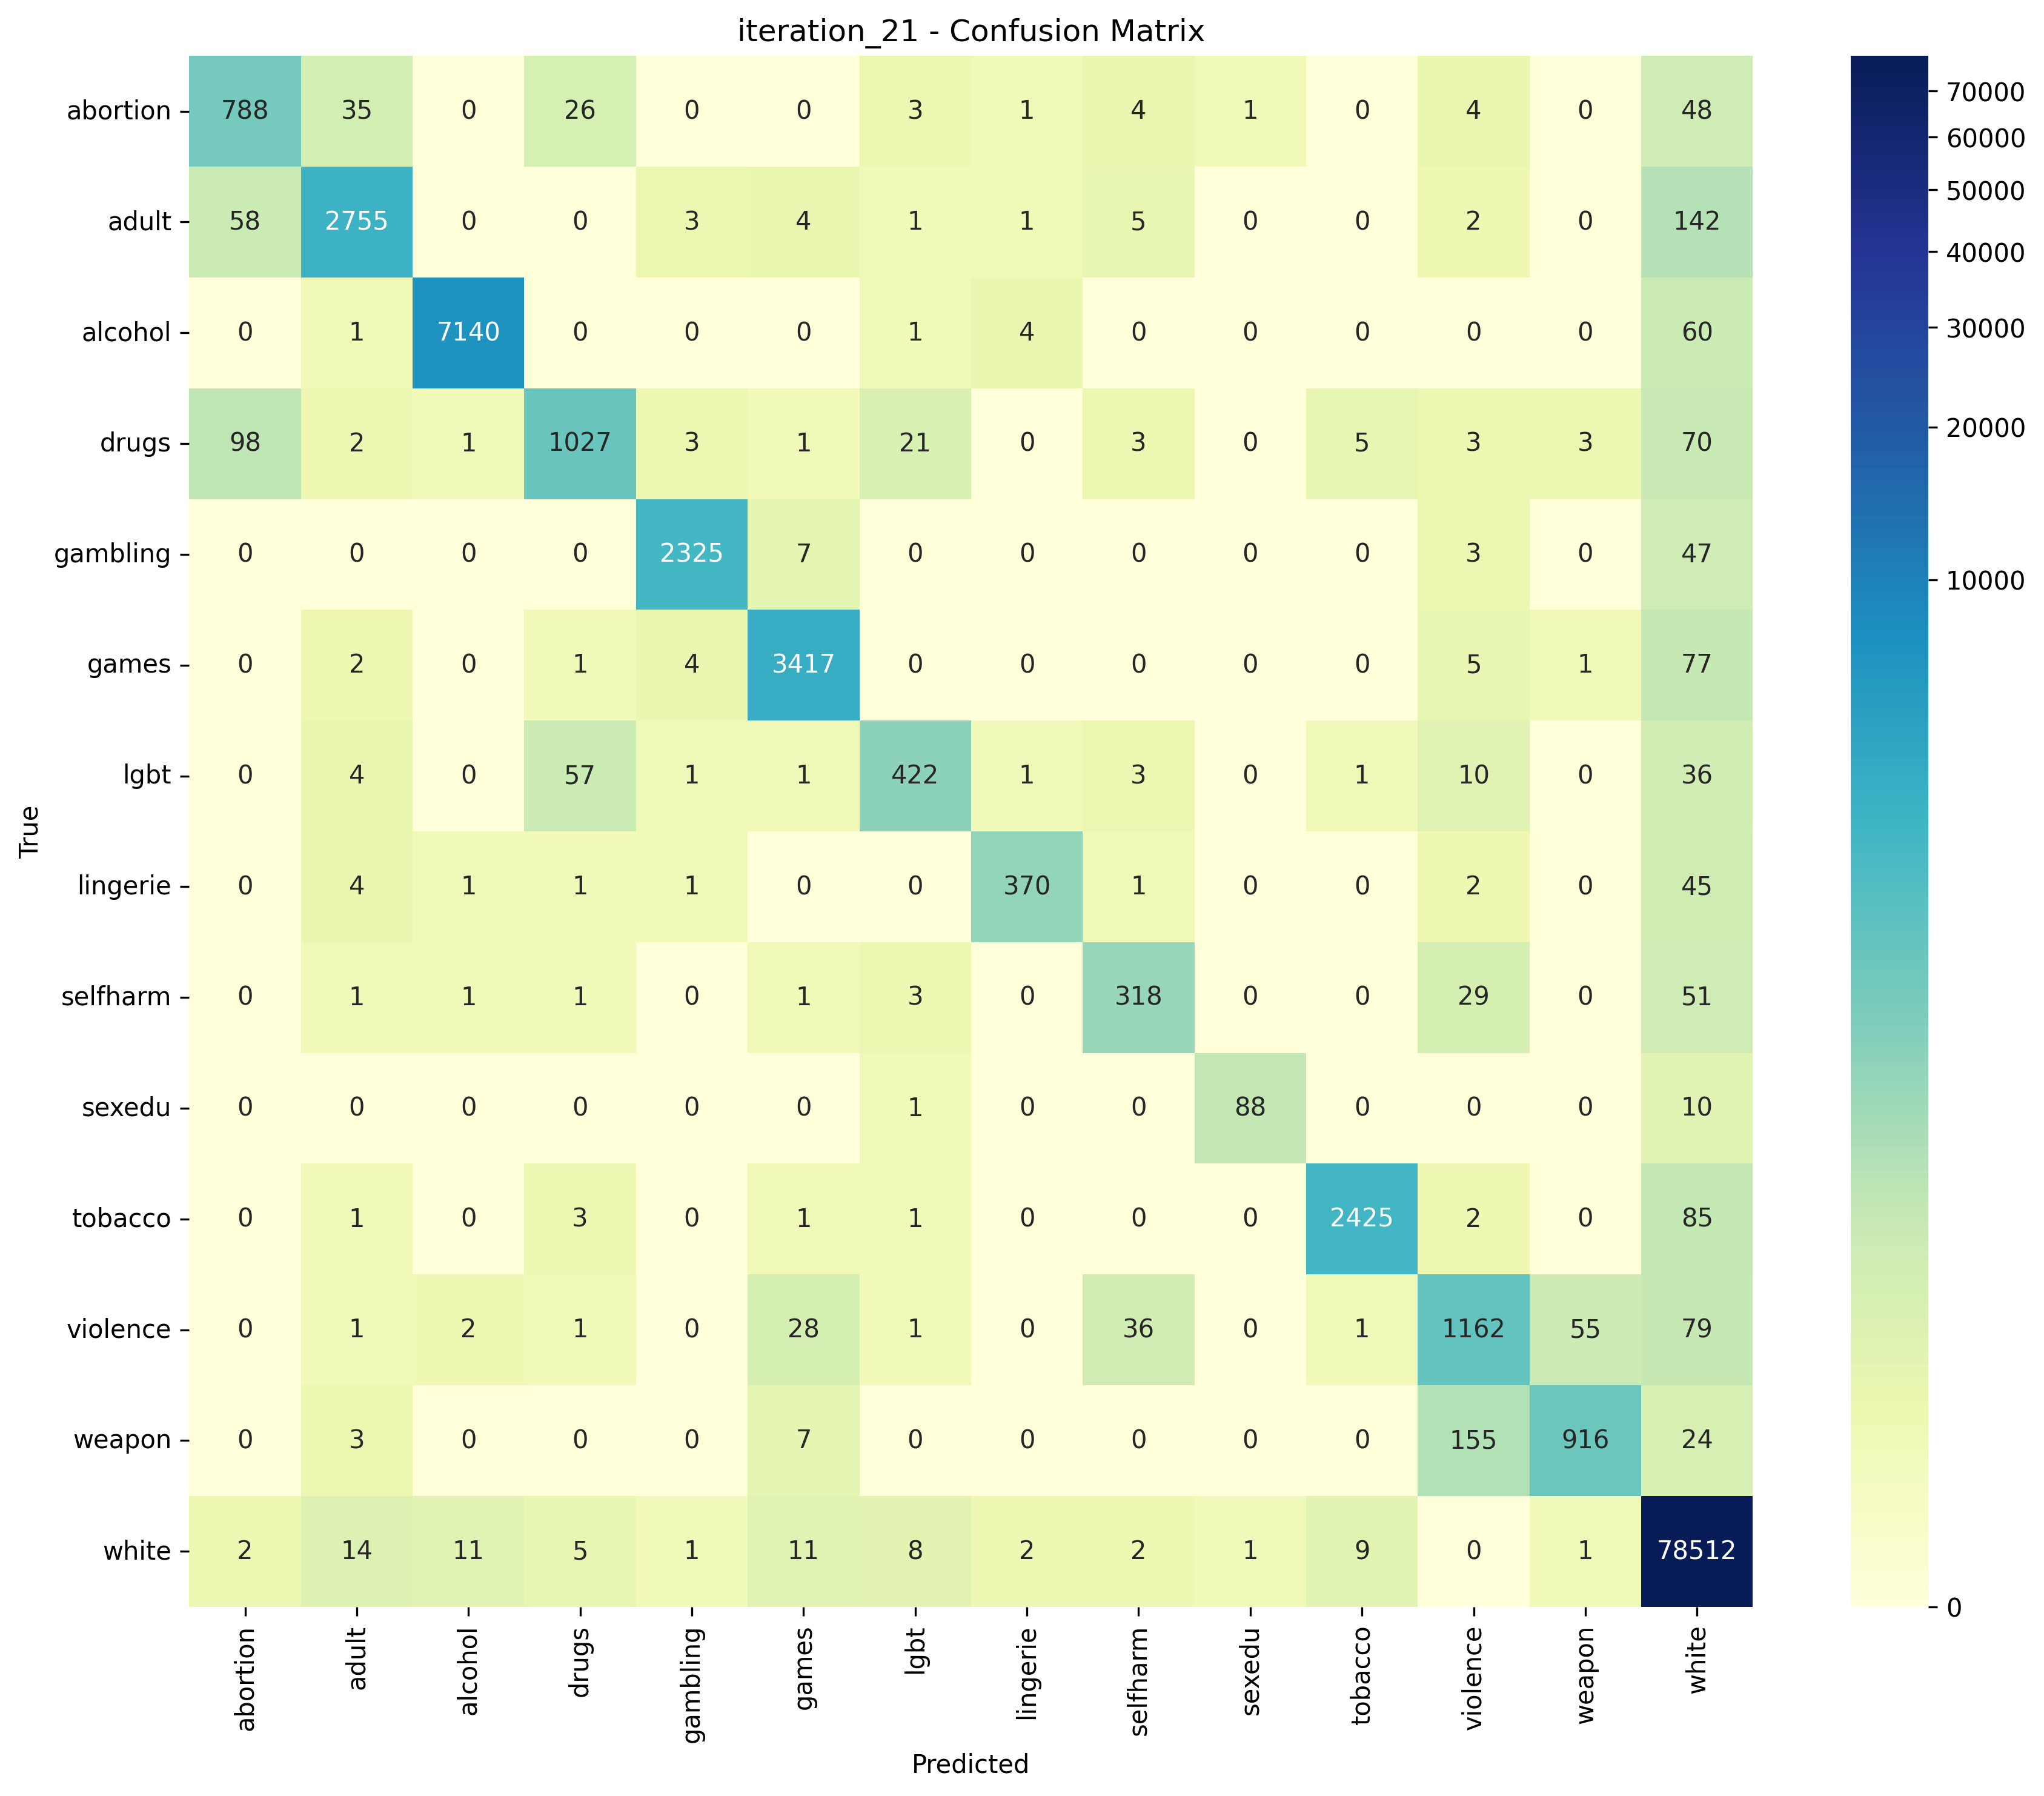
\includegraphics[keepaspectratio]{figures/21_iteration_21_confusion_matrix.png}}

}

\caption{Confusion matrix of iteration \#21 for XGBoost localized
hyperparameter search with custom hyperparameter weights.}

\end{figure}%

\subsection{LinearSVC}\label{linearsvc-1}

\begin{figure}

\begin{minipage}{0.50\linewidth}

\begin{figure}[H]

{\centering \pandocbounded{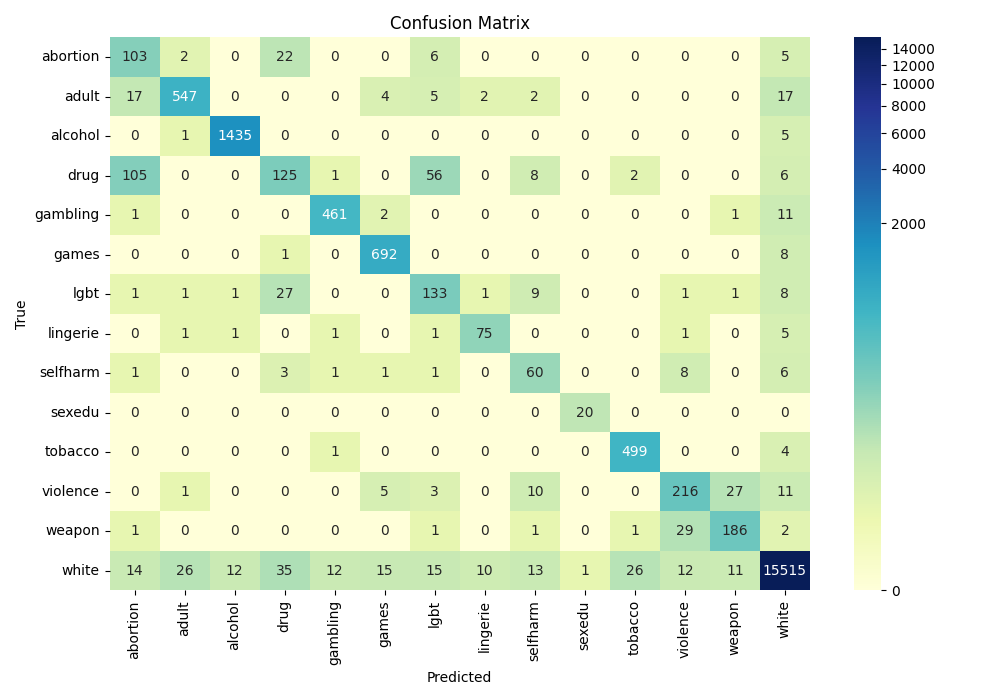
\includegraphics[keepaspectratio]{figures/22_v4_cm_cut.png}}

}

\subcaption{V4.0.0, setting \texttt{cut\_all} to \texttt{True}}

\end{figure}%

\end{minipage}%
%
\begin{minipage}{0.50\linewidth}

\begin{figure}[H]

{\centering \pandocbounded{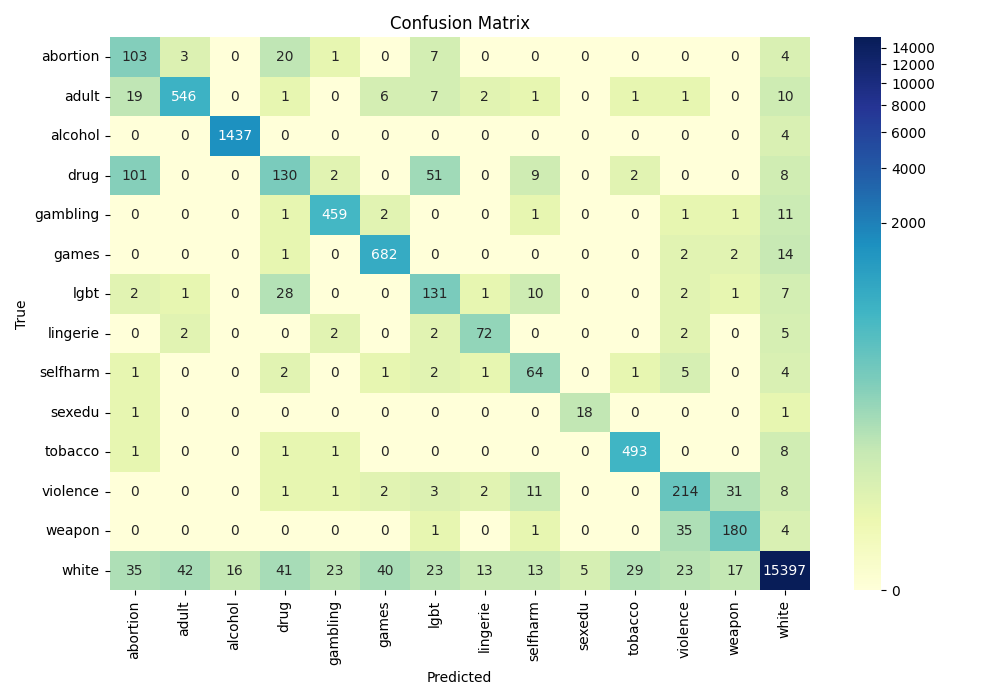
\includegraphics[keepaspectratio]{figures/22_v4_cm_search.png}}

}

\subcaption{V4.0.0, using the \texttt{cut\_for\_search} mode}

\end{figure}%

\end{minipage}%

\end{figure}%

Initially, the baseline model of choice was LinearSVC, implemented with
both vectorized text using jieba's \texttt{cut\_all} and
\texttt{cut\_for\_search} mode. These two methods demonstrated poor
performance with a F1-macro score of 0.8065 for the \texttt{cut\_all}
method and similar performance for the \texttt{cut\_for\_search} method
before vectorization. It was during this time that there were a few
outlier confusion categories, namely abortion and drugs, as well as
drugs and lgbt.

\begin{figure}[H]

{\centering \pandocbounded{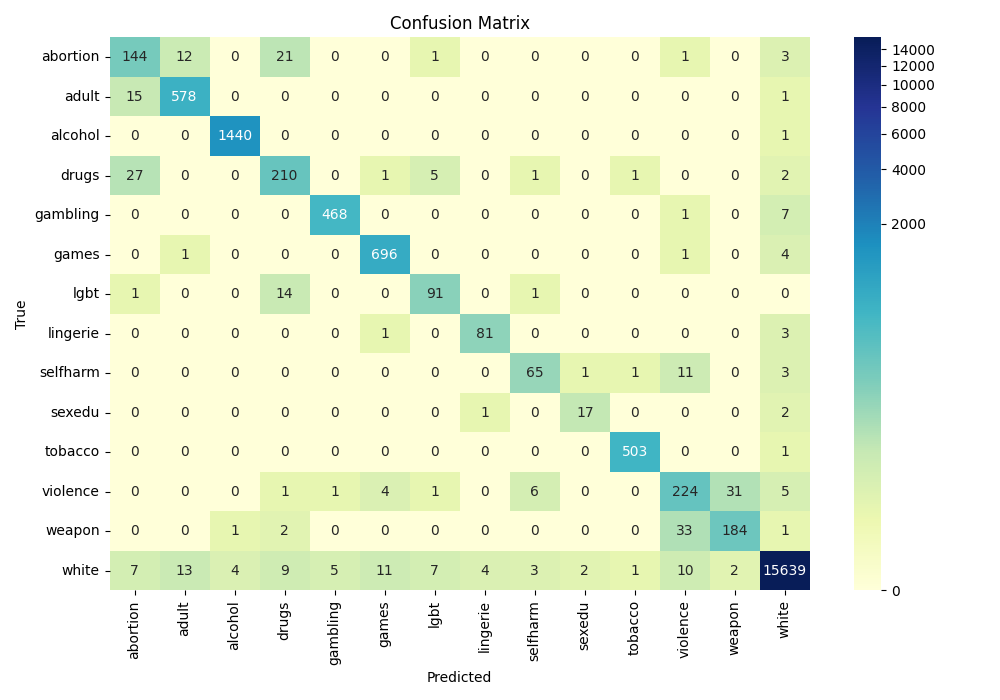
\includegraphics[keepaspectratio]{figures/23_v4.4.0_cm.png}}

}

\caption{V4.4.0 confusion matrix for train set after processing
confusion category data.}

\end{figure}%

After using two LLMs and a suitable prompt to adjust the labels of the
aforementioned categories, our vectorizer was also recalibrated with the
adjusted vectorizer dictionary, resulting in a significant performance
increase for our LinearSVC model (F1-macro score of 0.9040).

\begin{figure}[H]

{\centering \pandocbounded{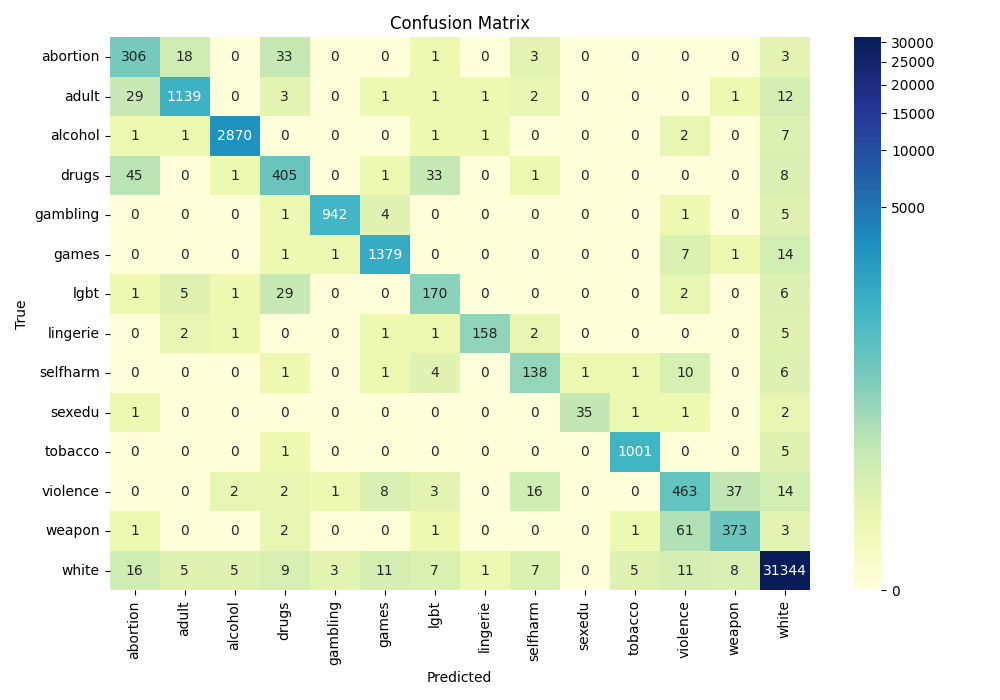
\includegraphics[keepaspectratio]{figures/24_v4.4.3_holdout_cm.png}}

}

\caption{V4.4.3 holdout set confusion matrix after data and vectorizer
recalibration.}

\end{figure}%

A final LinearSVC model was trained using optimal parameters including
l2 regularization, and a 8/1/1 train/test/holdout split, demonstrating
the model's ability to generalize to a holdout dataset and performance
on-par with other model candidates.

\begin{figure}[H]

{\centering \pandocbounded{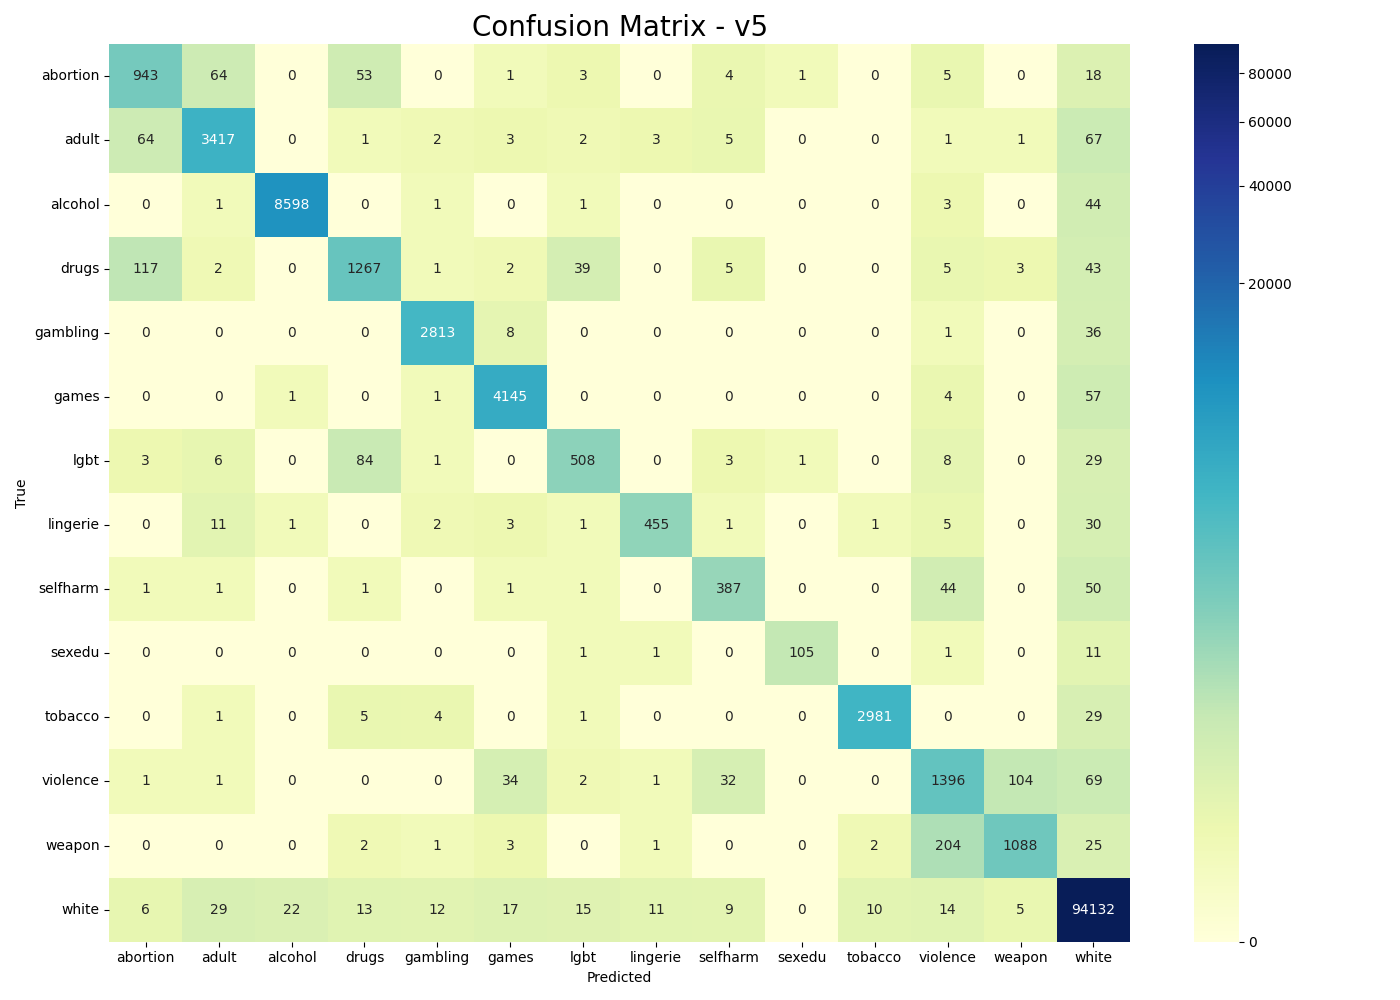
\includegraphics[keepaspectratio]{figures/25_v5_confusion_matrix.png}}

}

\caption{Confusion matrix for version 5 (final version) of our LR
model.}

\end{figure}%

\subsection{Logistic Regression}\label{logistic-regression-1}

At this point during the model selection process, both the vectorizer
dictionary and the existing issue of the mislabeled data has already
been solved. Initial model performance with minimal hyperparameter
tuning resulted in an F1-macro score of 0.8955, with one subsequent tune
for high recall achieving a recall-macro score of 0.9592. However, the
best performing model to date achieved an F1-macro score of 0.9183,
precision-macro of 0.9341 and recall-macro of 0.9040, on par with the
performance of other model finalists.

\begin{figure}[H]

{\centering \pandocbounded{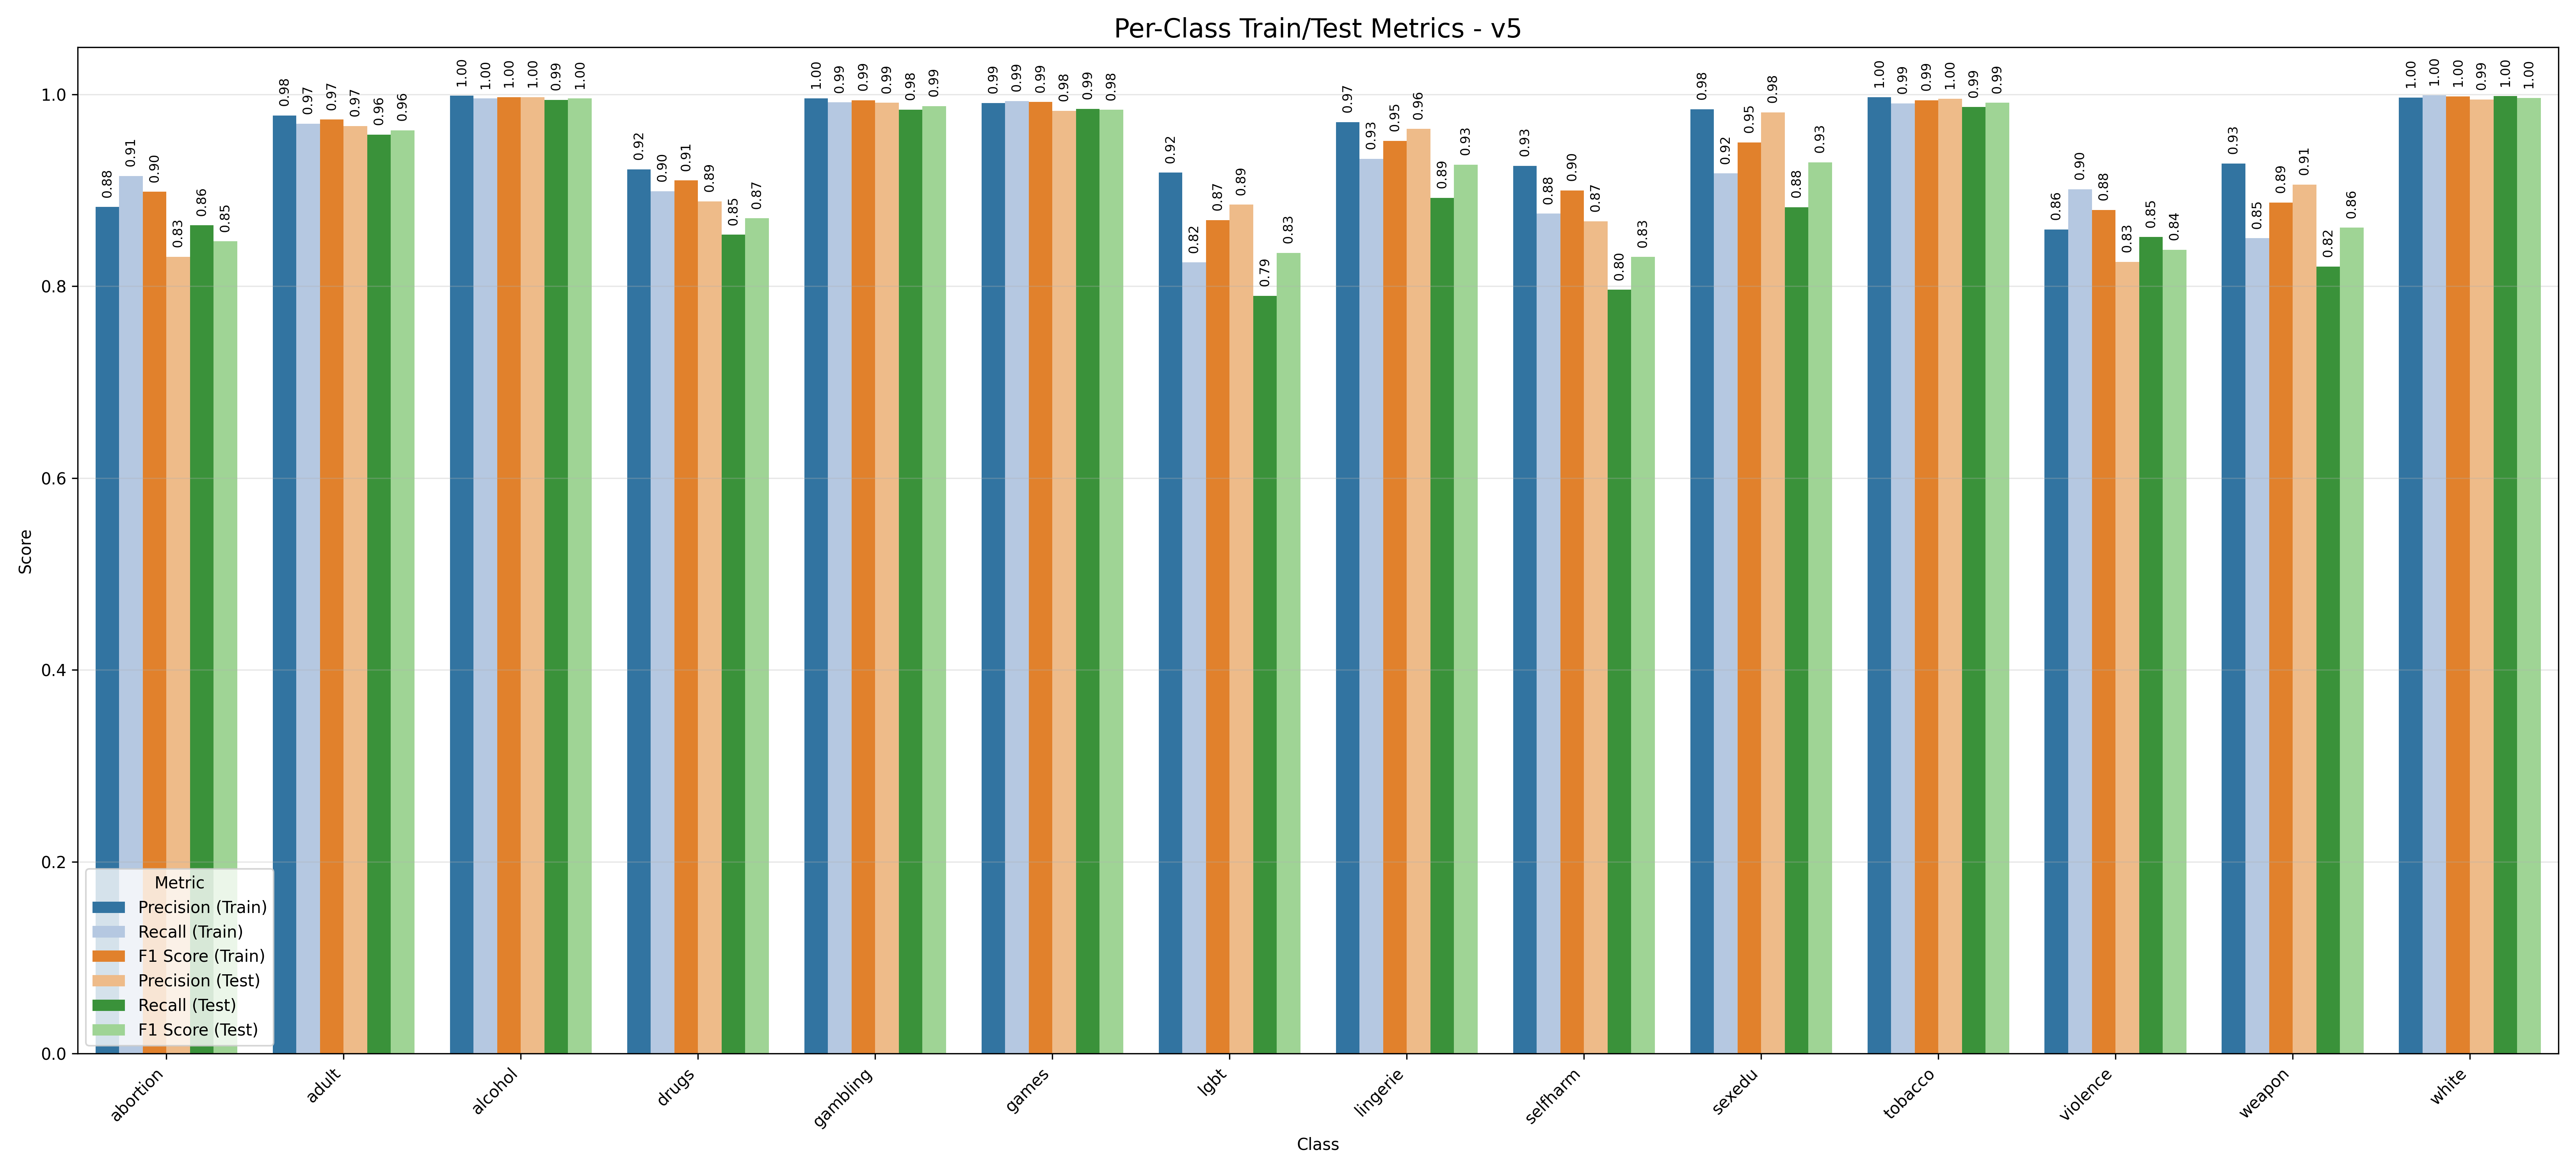
\includegraphics[keepaspectratio]{figures/26_v5_per_class_metrics_train_test.png}}

}

\caption{Per Class train-test F1-macro, precision-macro, and
recall-macro values for V5 (final) version of our LogisticRegression
model compared to previous versions.}

\end{figure}%

\subsection{Model Selection}\label{model-selection}

\subsubsection{Comparing XGBoost, LR, LinearSVC, and LR Confusion
Matrices.}\label{comparing-xgboost-lr-linearsvc-and-lr-confusion-matrices.}

\begin{figure}[H]

{\centering \pandocbounded{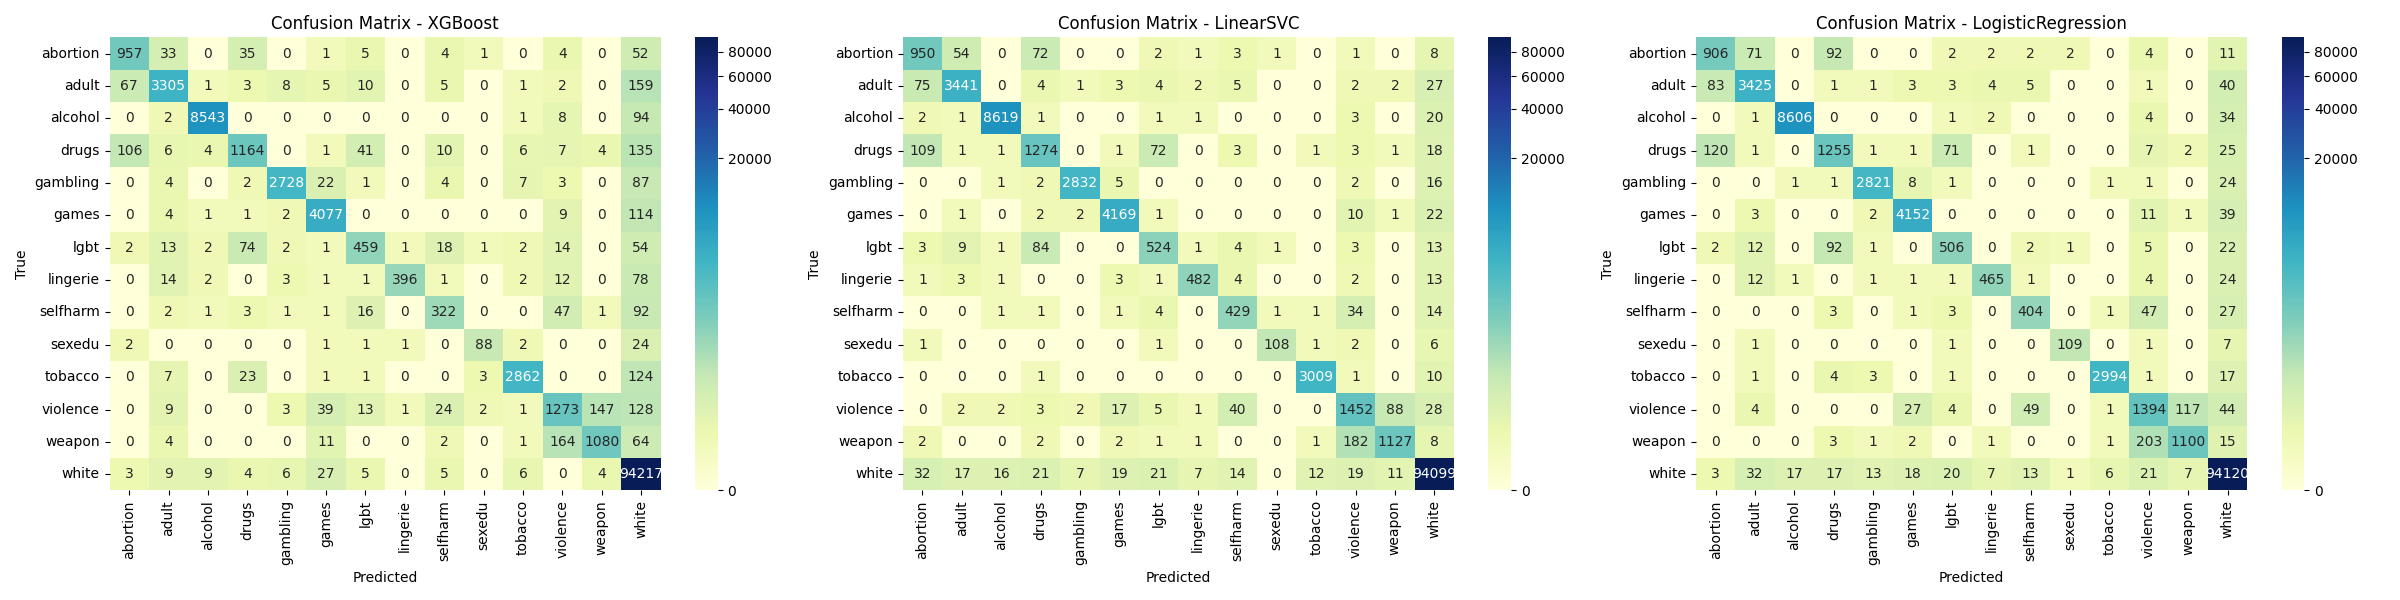
\includegraphics[keepaspectratio]{figures/27_v4.6.3_cm_comparison.png}}

}

\caption{Comparing XGBoost, LR, LinearSVC, and LR Confusion Matrices.}

\end{figure}%

A closer look at the confusion matrices reveals fundamental differences
in how each model approaches the classification task. The precision
vs.~recall scatter plot demonstrates that LinearSVC achieves
consistently high precision across most categories while maintaining
competitive recall, doing particularly well in categories with moderate
support sizes such as tobacco, gambling, and adult content. XGBoost,
while showing strong performance in high-support categories like alcohol
and games, struggles to generalize in minority classes with several
categories falling below the precision-recall diagonal. This pattern
suggests that XGBoost's ensemble approach, while powerful for balanced
datasets, struggles with the extreme class imbalance of our dataset.

\begin{figure}[H]

{\centering \pandocbounded{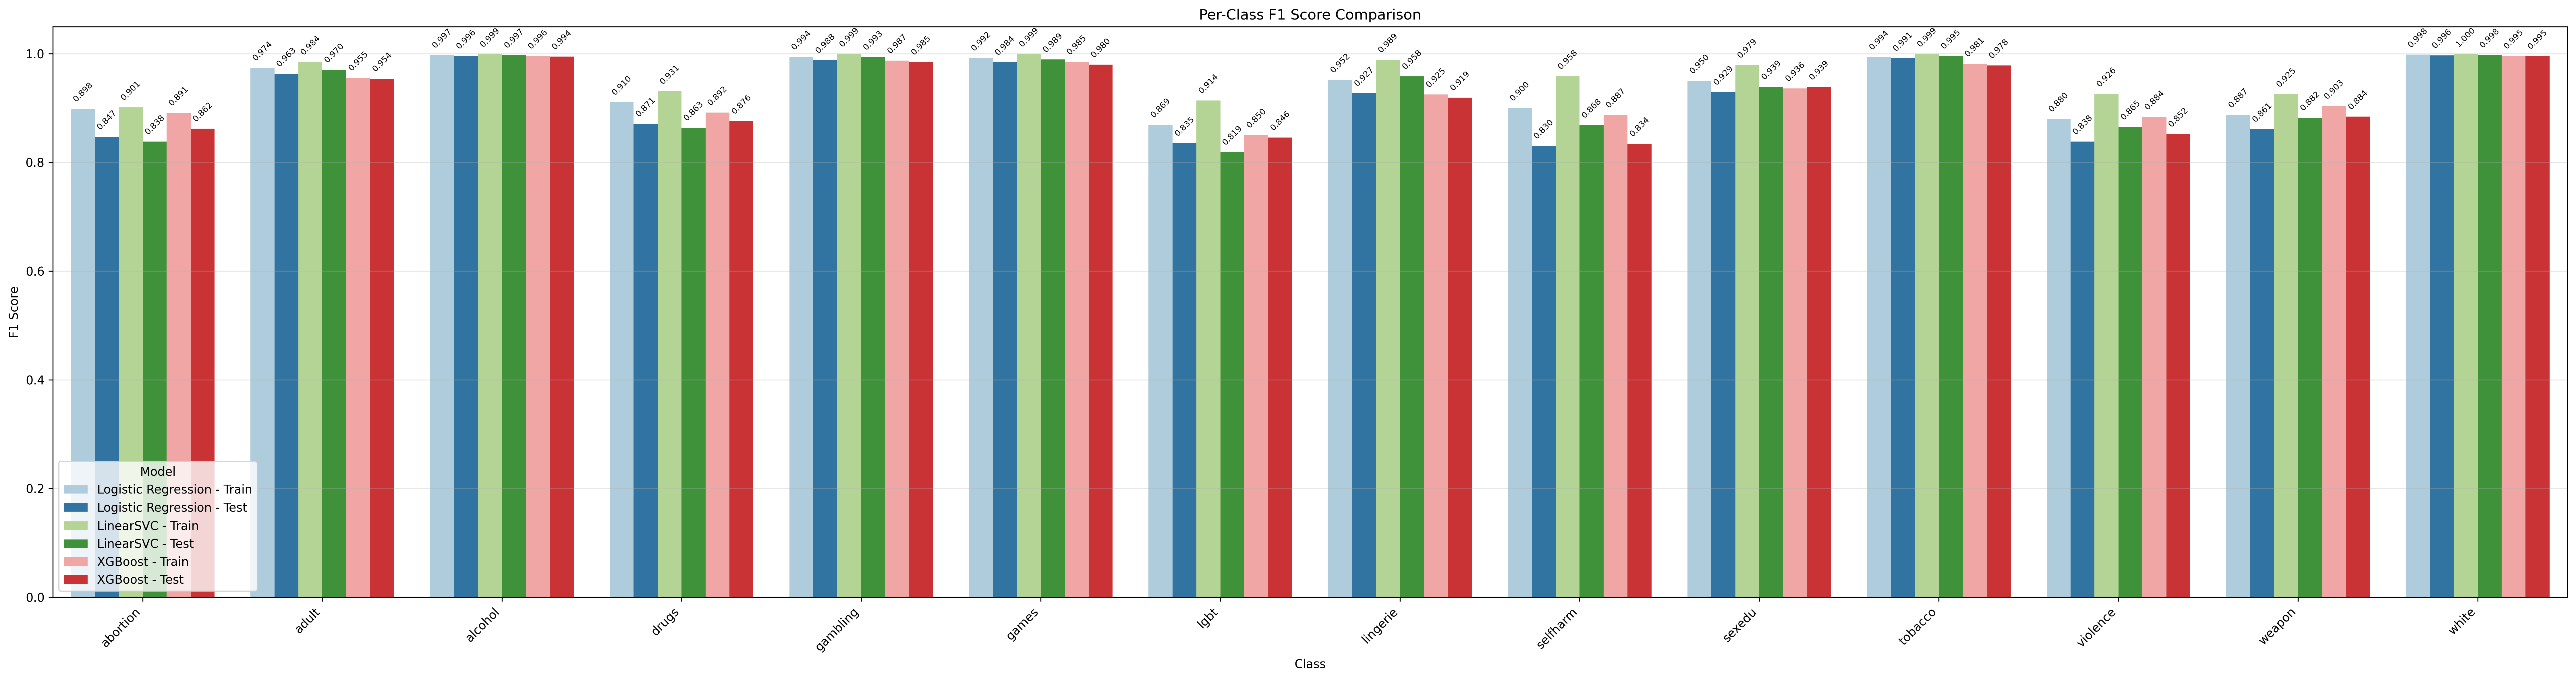
\includegraphics[keepaspectratio]{figures/28_v4.9.1_combined_comparison_f1-score.png}}

}

\caption{Comparing XGBoost, LR, and LinearSVC train-test performances by
category.}

\end{figure}%

\begin{figure}[H]

{\centering \pandocbounded{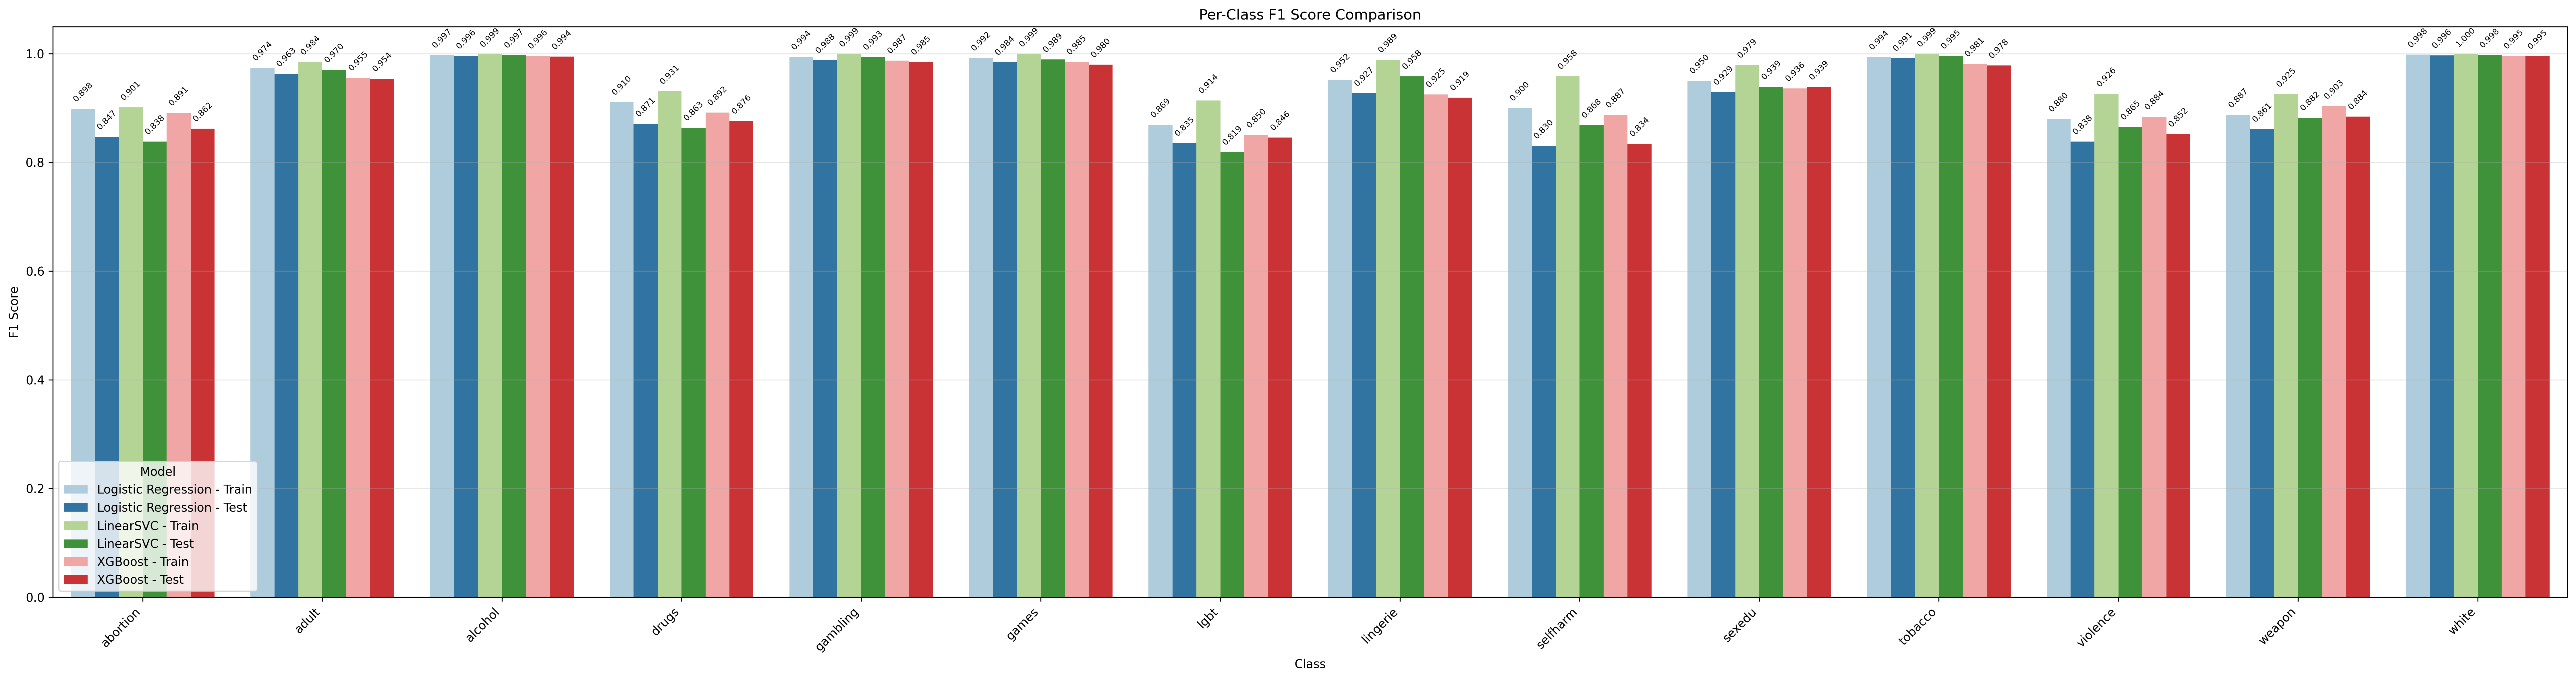
\includegraphics[keepaspectratio]{figures/28_v4.9.1_combined_comparison_f1-score.png}}

}

\caption{Comparing XGBoost, LR, and LinearSVC test performances by
category, support size per category.}

\end{figure}%

LinearSVC demonstrates the most consistent performance gap between
training and testing phases, indicating robust generalization
capabilities essential for real-world educational environments where
content patterns may differ from training distributions. Conversely,
XGBoost shows larger train-test disparities across multiple categories,
particularly in self-harm, violence, and weapons classification,
suggesting potential overfitting despite regularization efforts.
Logistic Regression strikes a middle ground, showing moderate
overfitting patterns but maintaining stable performance across
categories with varying support sizes. Given the deployment constraints
of client-side inference on resource-limited devices and the critical
need for consistent classification decisions in educational settings,
these generalization characteristics heavily favor linear approaches
over ensemble methods.

\subsubsection{Final Model}\label{final-model}

\begin{figure}[H]

{\centering \pandocbounded{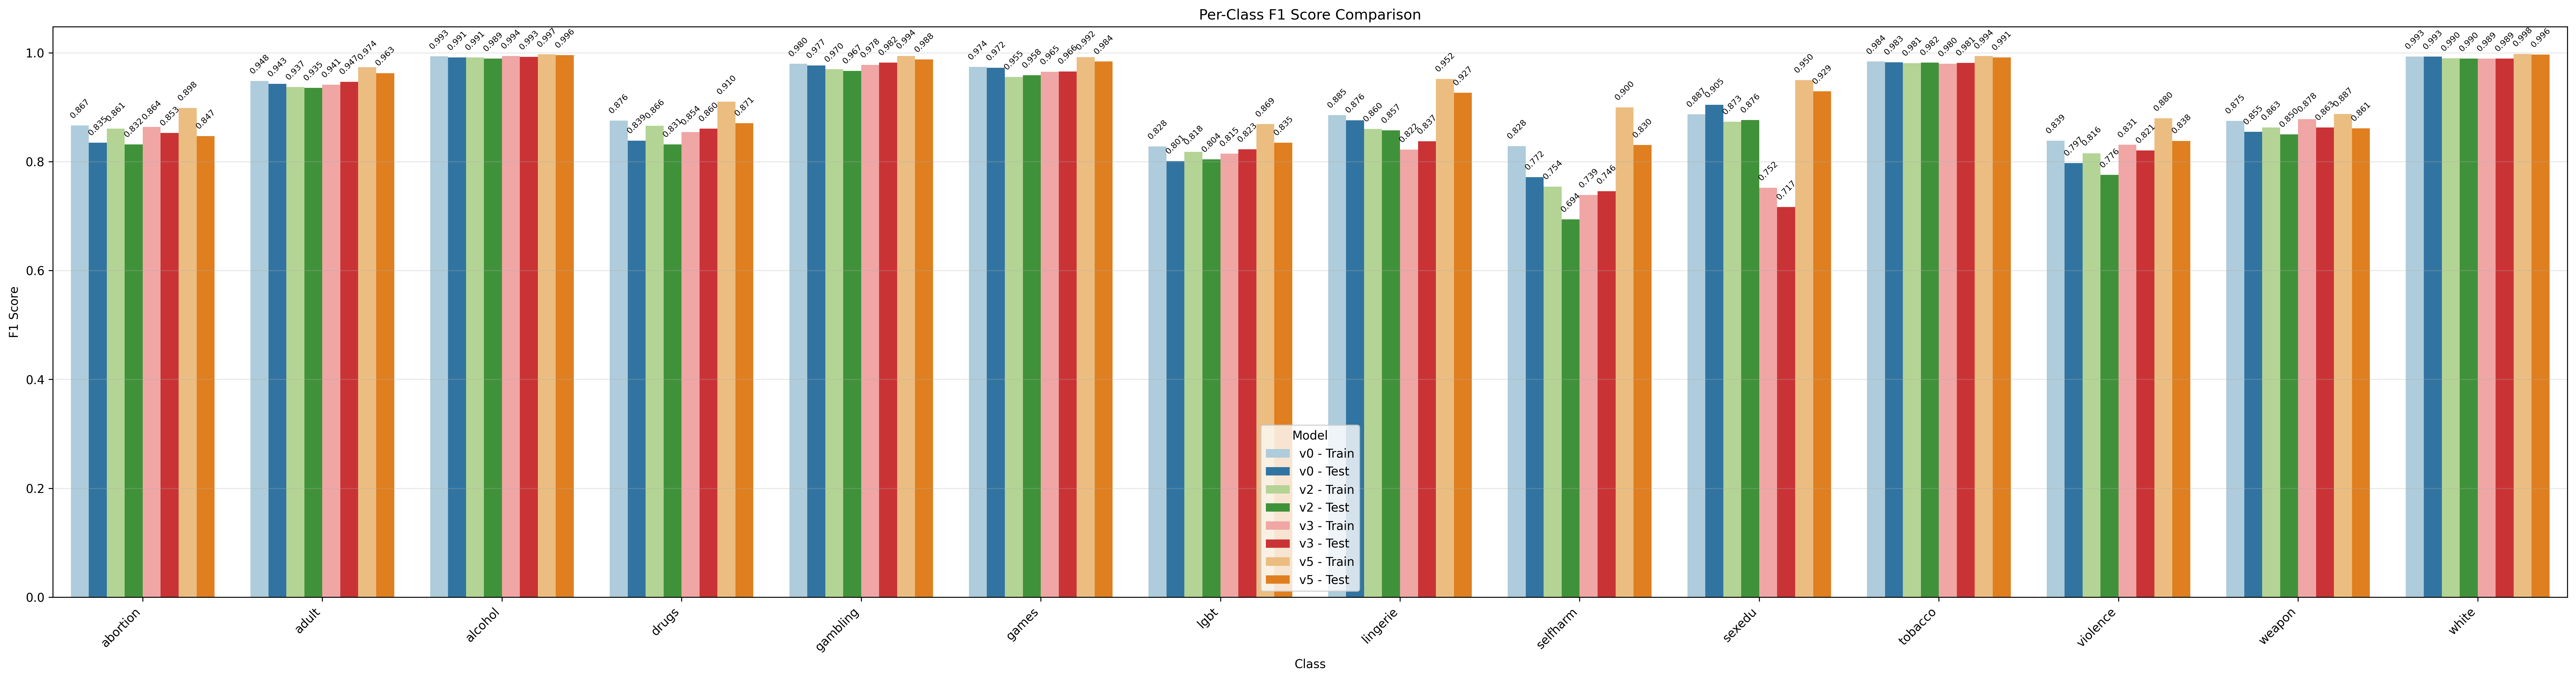
\includegraphics[keepaspectratio]{figures/29_v4.9.2_combined_comparison_f1-score.png}}

}

\caption{Per-class train--test F1-macro score comparison for Logistic
Regression model candidates: v0 (initial baseline), v2/v3 (optimized for
high recall), and v5 (optimized for F1-macro performance).}

\end{figure}%

The progression from V0 to V5 demonstrates systematic improvement in
both overall performance and category-specific classification accuracy.
The f1-macro result analysis reveals that V5 achieves superior balance
compared to earlier iterations, particularly evident in challenging
categories such as self-harm, violence, and weapons where V2/V3 models
optimized for high recall showed significant precision degradation.

\begin{figure}[H]

{\centering \pandocbounded{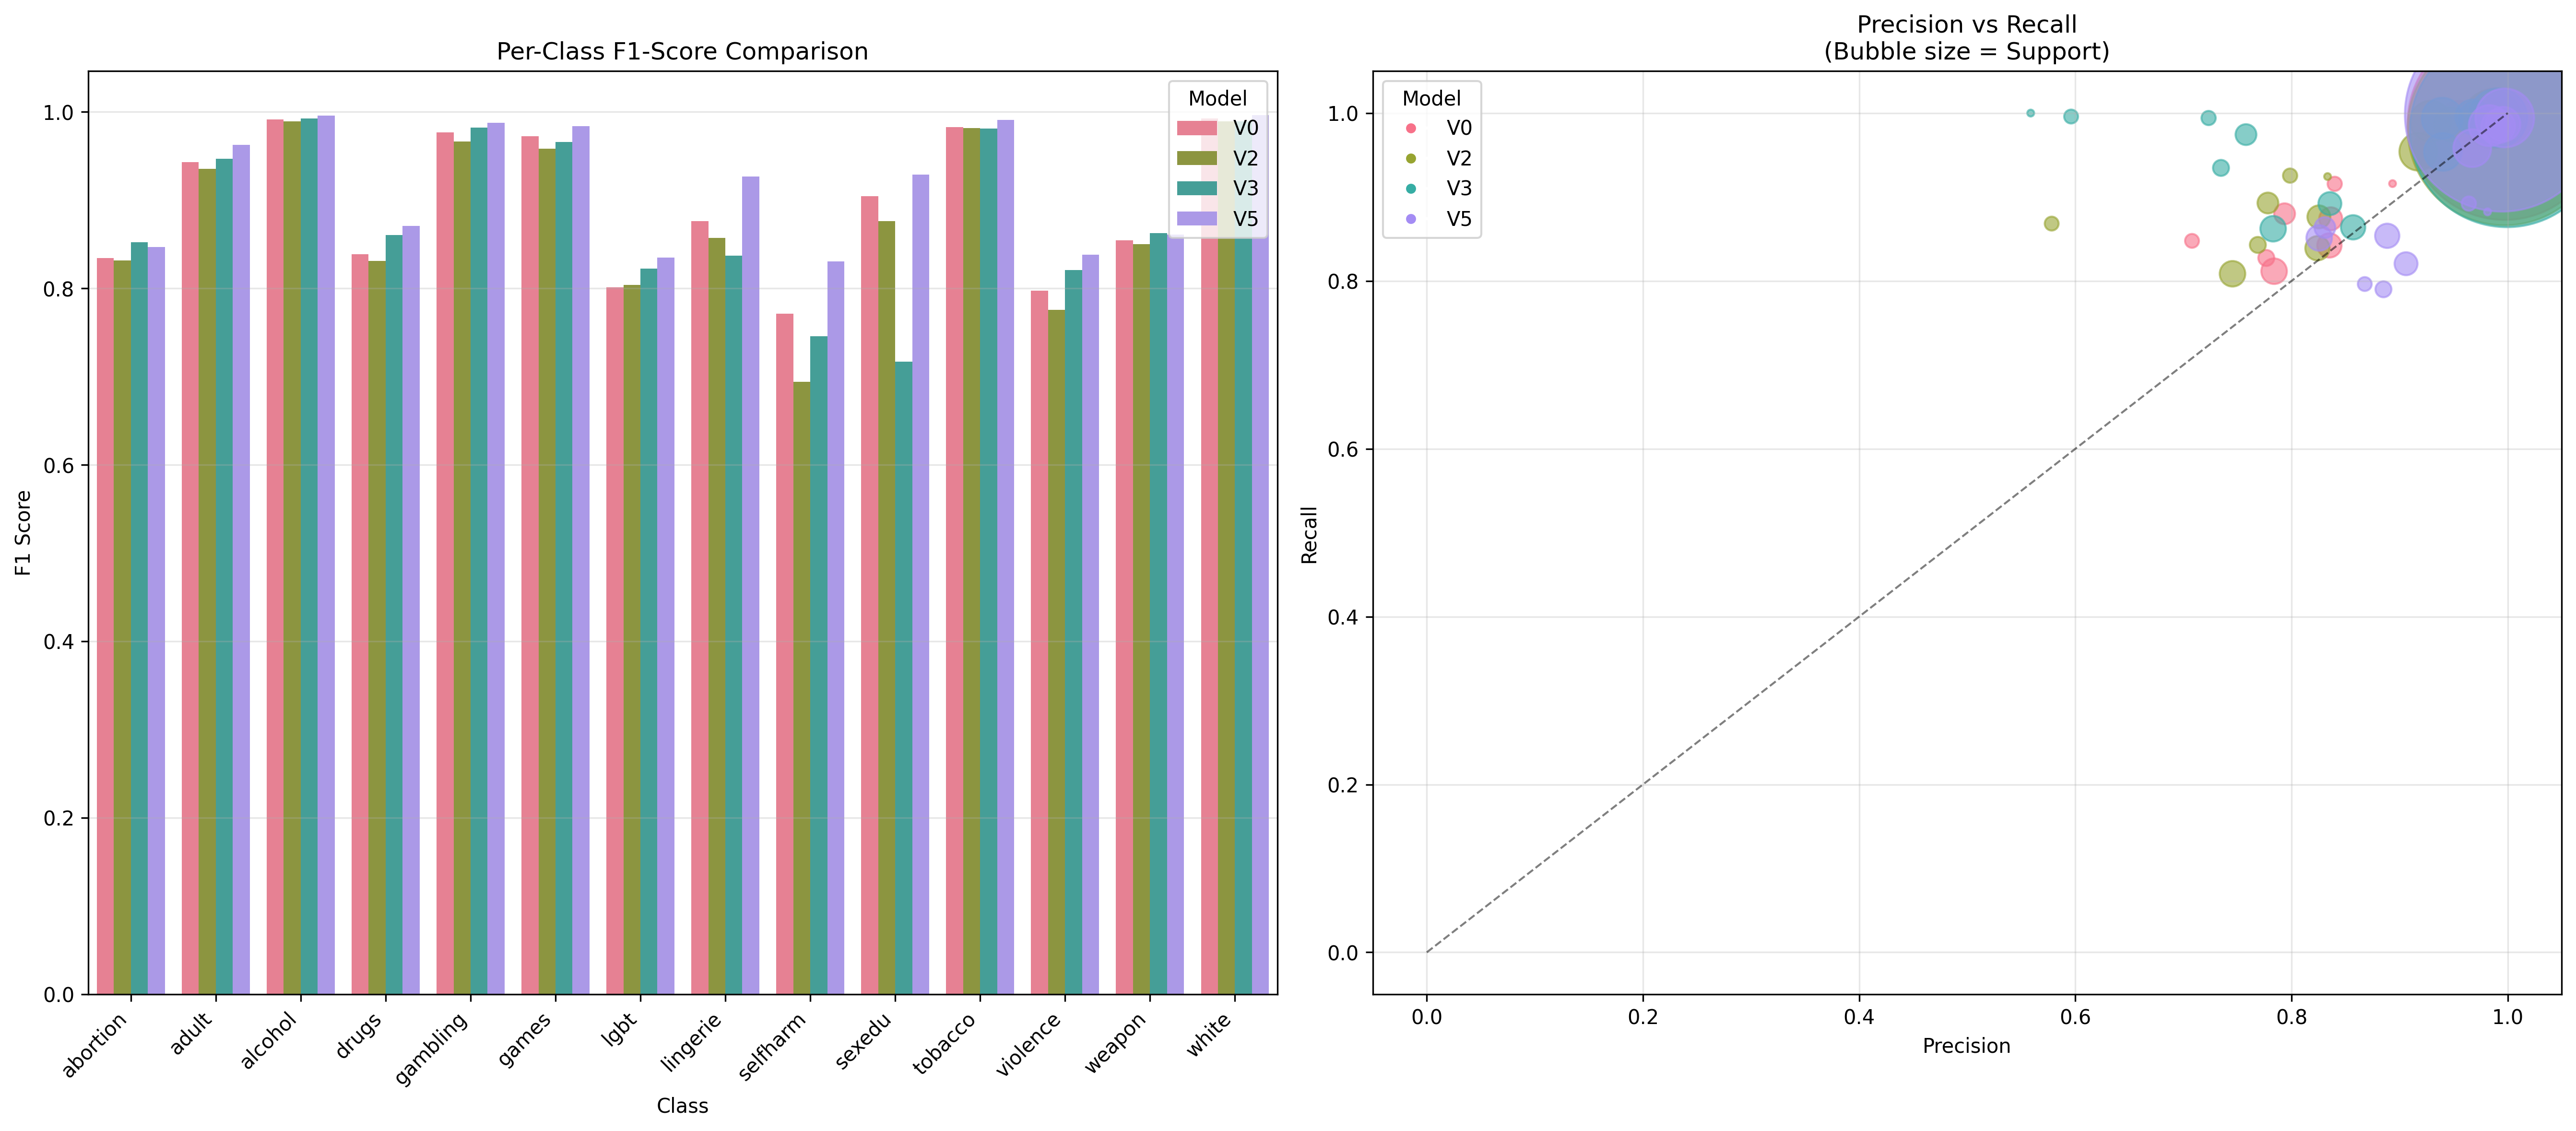
\includegraphics[keepaspectratio]{figures/29_v4.9.2_comparison_performance_summary.png}}

}

\caption{Per-class test F1-macro score comparison with recall--precision
trade-off and class support indication for Logistic Regression model
candidates: v0, v2/v3, and v5.}

\end{figure}%

The bubble size visualization indicates that V5 maintains competitive
performance across categories with varying support sizes, addressing the
dataset imbalance challenges that plagued earlier versions. Notably, V5
shows marked improvement in minority classes like sexedu and lingerie
while preserving strong performance in high-support categories such as
alcohol and games, indicating successful regularization that prevents
the model from overfitting to majority classes.

\begin{figure}[H]

{\centering \pandocbounded{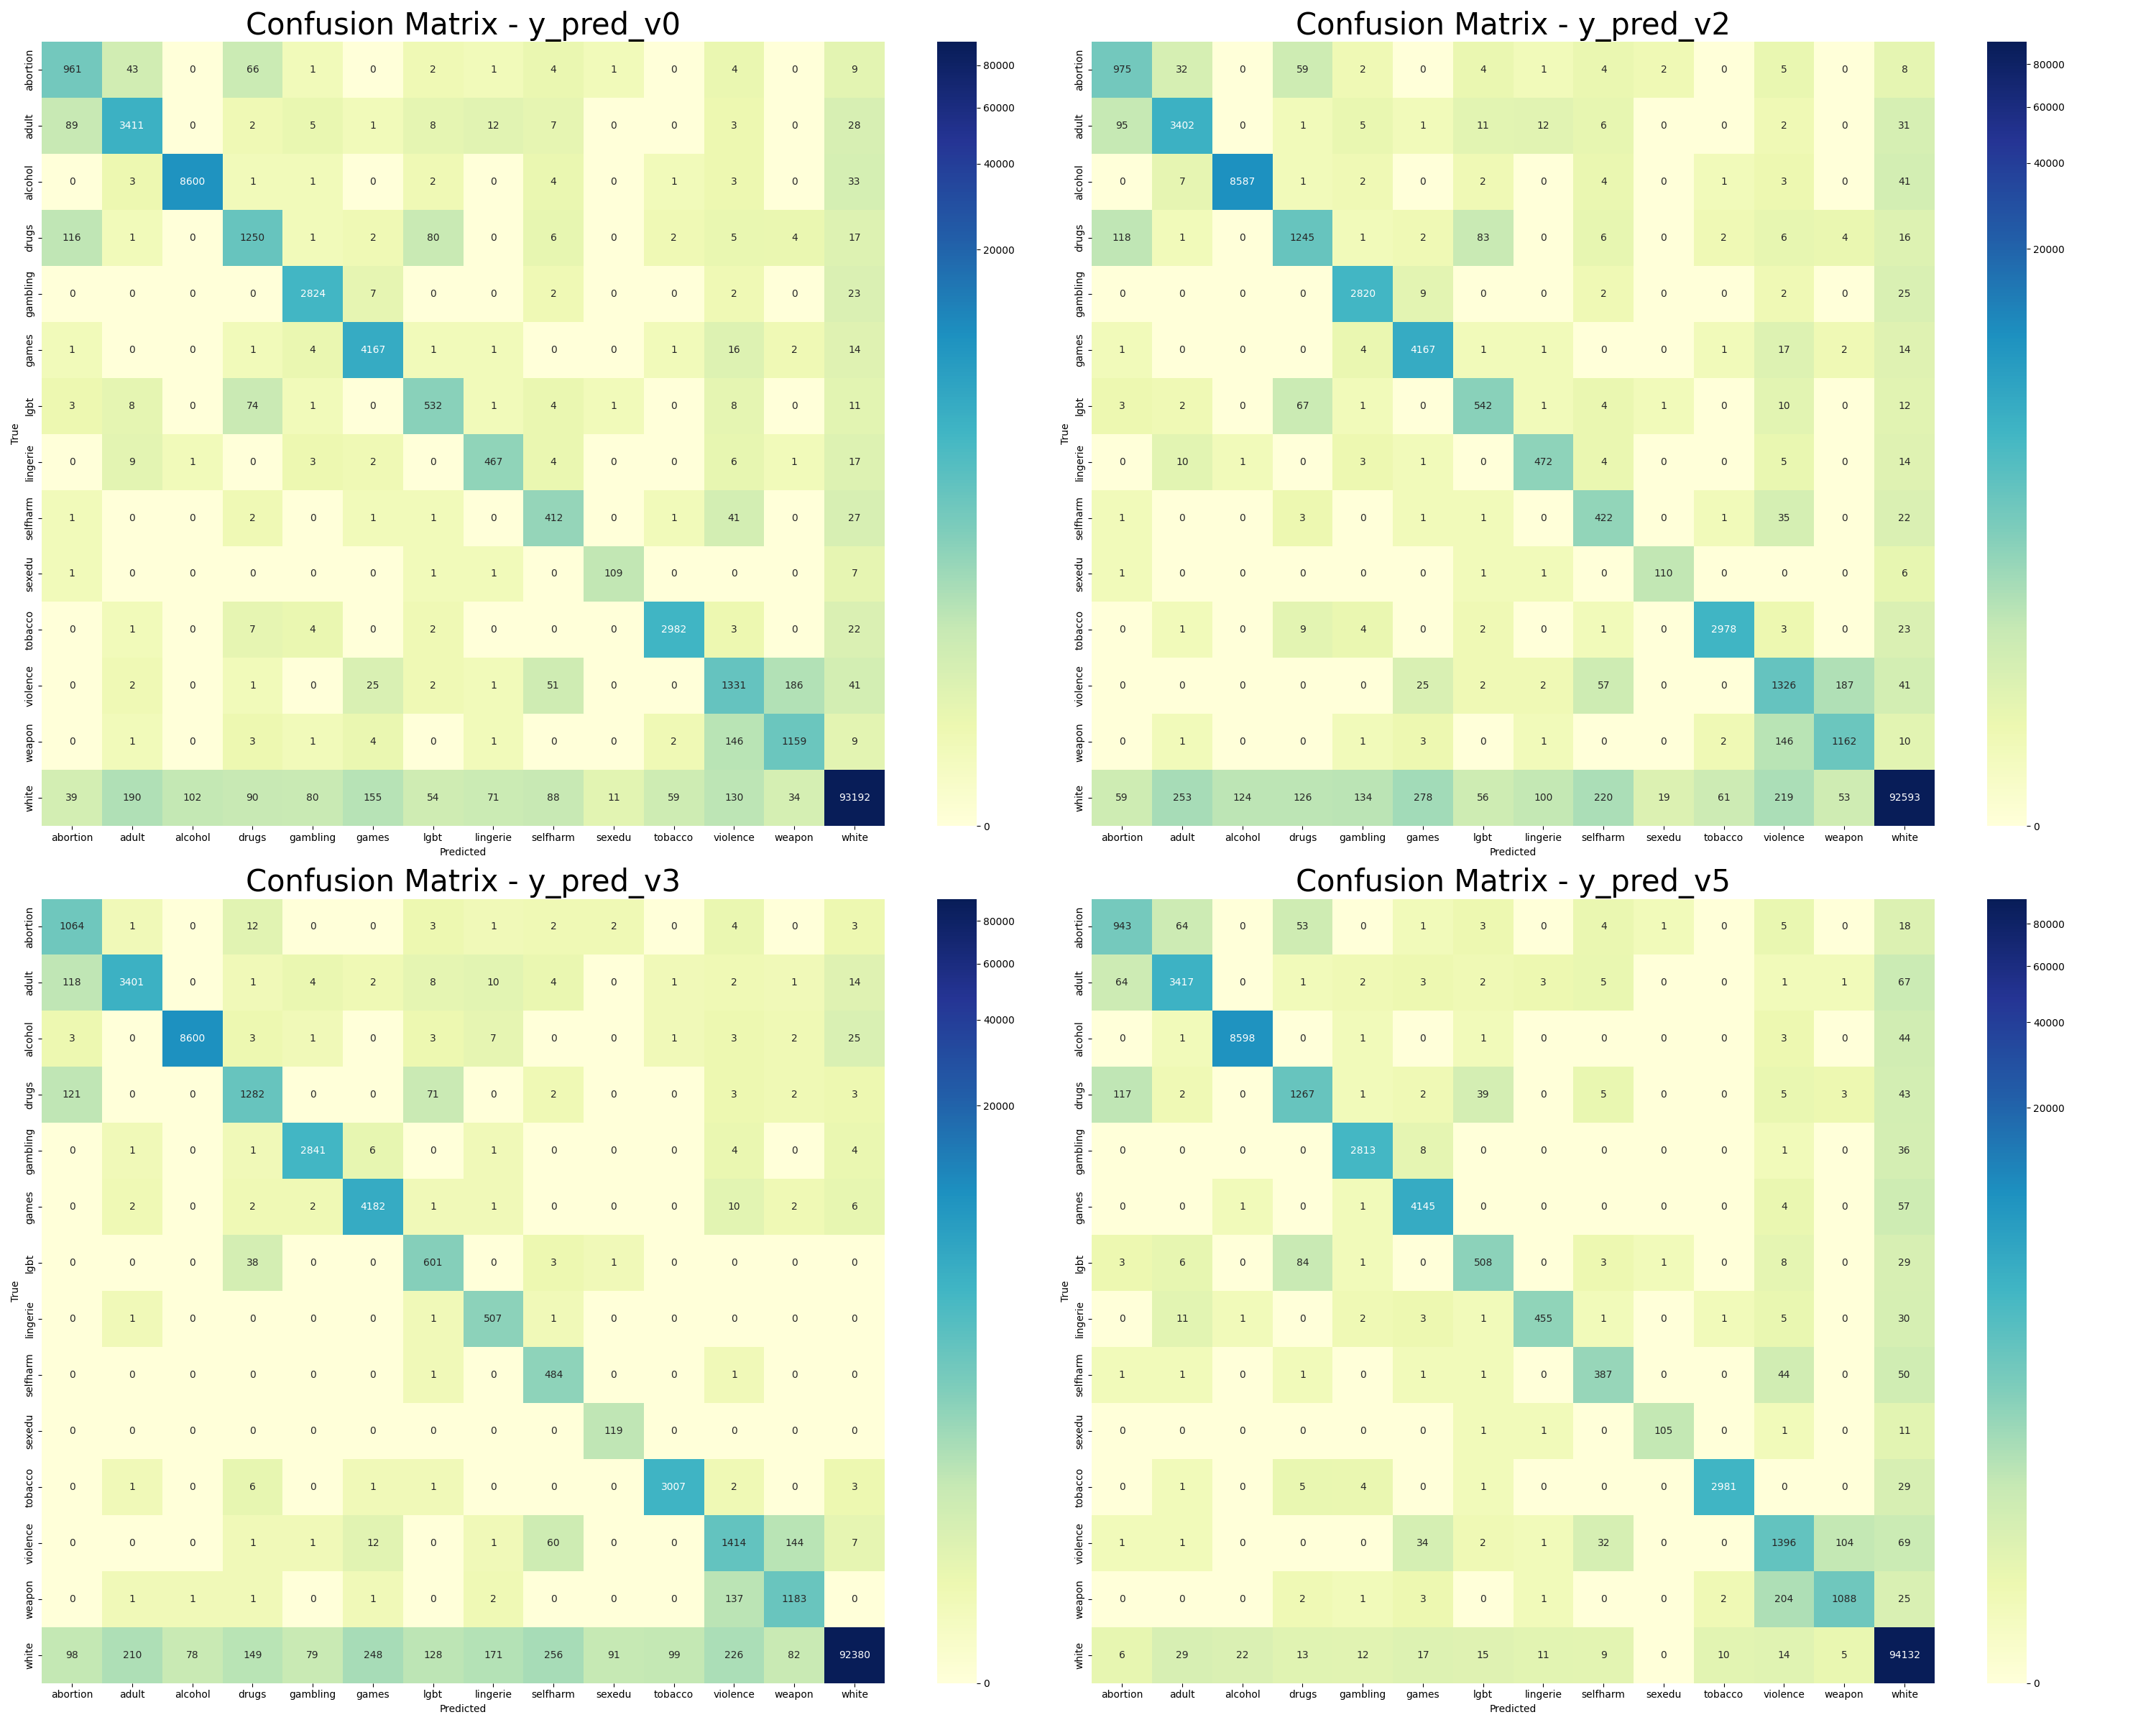
\includegraphics[keepaspectratio]{figures/29_v4.9.2_test_cm_comparison.png}}

}

\caption{Confusion matrices for the top 4 Logistic Regression model
candidates, comparing classification performance across classes.}

\end{figure}%

V5 demonstrates substantially cleaner diagonal patterns compared to V0,
with significant reduction in off-diagonal misclassifications that
characterized earlier versions. The most pronounced improvements appear
in previously problematic category pairs, such as the reduction of
drugs-lgbt confusion and the better separation of adult content from
lingerie classifications. This enhanced discrimination capability stems
from the optimized regularization parameters. The consistent train-test
performance gaps across all model versions validate the generalization
capabilities, with V5 showing the most stable performance differential,
crucial for deployment in production environments where distribution
shift is expected.

From a deployment perspective, the V5 configuration represents an
optimal compromise between computational efficiency and classification
accuracy for client-side implementation. The relatively low
regularization strength (C=220.77) allows the model to capture complex
feature interactions necessary for distinguishing between nuanced
Chinese content categories during training, while the L2 penalty
prevents overfitting to the specific linguistic patterns in our training
corpus. The surprisingly low 154-iteration convergence profile indicates
that the stopping threshold was reached rather early and did not show
signs of gradient oscilation. This hyperparameter configuration,
combined with the multinomial approach, positions V5 as the foundation
model for CWCM deployment while maintaining compatibility with the
planned transformer-based CWCM-V2 secondary layer.

\section{Discussion}\label{discussion}

\subsection{Model Selection}\label{model-selection-1}

Linear methods in NLP have long been the norm given the complexity of
computational cost associated with non-linear methods and before the
arrival of advanced computing resources and methods during the previous
decade. While it may be tempting to reach for non-linear methods for
text classification, given the limitation of client-side computational
resources still relying on low-end CPUs and integrated graphics for
processing, we require a fast and efficient linear implementation of the
CWCM classifier, both during the initial stage of standalone model
deployment as well as during the second phase where CWCM works in
conjunction with CWCM-V2.

As seen during the initial phases of general model comparison and
selection, the Passive Aggressive Classifier (PAC) exhibited the best
raw performance with untuned hyperparameters (Crammer et al., 2006).
While scikit-learn's implementation of PAC is a method wrapper around a
linear model, what is interesting to note is that both PAC and LinearSVC
share the same hinge loss function. While there are some non-trivial
differences between squared hinge and hinge loss, the loss function no
longer considers a datapoint relevant to updating the models parameters
once a datapoint has been correctly classified, contributing to how the
model effectively generalizes to unseen data in production (Lee \& Lin,
2013). The shared loss function means that while the two models are not
identical in practice, they are both linear models that share enough
traits to substitute one for the other during training. In addition,
LinearSVC also has the additional advantage of being particularly robust
to previously unseen data as it relies on support vectors as its method
of classification.

\begin{figure}[H]

{\centering \pandocbounded{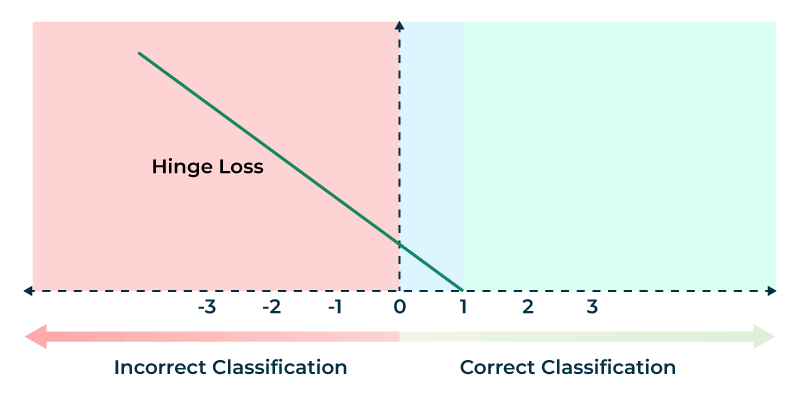
\includegraphics[keepaspectratio]{figures/hinge_loss.png}}

}

\caption{Hinge Loss in SVM (GeeksforGeeks, 2025)}

\end{figure}%

This is what sets the final LinearSVC candidate apart from the two other
modes, one being Logistic Regression (linear model using cross entropy
loss) and the other being XGBoost (boosted decision tree model also
using categorical cross-entropy loss), both of which did not outperform
the former. It is also worth noting that while during testing that the
LinearSVC model performs slightly better in terms of F1-macro score
(0.9270) against Logistic Regression V5 (0.9183) as well as XGBoost \#21
(0.9177) even without custom model weights that emphasise the confusion
categories. However, while using custom weights for LinearSVC did go
unexplored and despite the slight empirical advantage of LinearSVC's
F1-macro score, we still opted for Logistic Regression due to the ease
of explainability of model performance as well as the fact that hinge
loss focuses on accuracy and margin maximization and not predicting
probabilities, which plays a significant role in adjusting sensitivities
during model deployment. At the same time, while there might be some
academic significance behind a 1-2\% increase in model performance, this
difference is almost rendered obsolete during production as most linear
models tend to overfit and degrade significantly in performance once
deployed, especially given the performance of the current CWCM model
(Mutsam et al., 2024).

\subsection{Logistic Regression vs the
Rest}\label{logistic-regression-vs-the-rest}

Before diving into the statistical significance of the model itself,
there is a noteworthy characteristic of the current model to discuss. It
relates to choosing the multinomial solving algorithm for multi-class
classification as opposed to using the one-vs-rest (OVR) method. As we
know, multinomial regression assumes the Independence of Irrelevant
Alternatives (IIA), which is difficult to achieve in real-world
applications, especially when it comes to NLP classification tasks.
However, despite the theoretical disadvantage of using multinomial
classification and the former CWCM model using OVR as a solving method,
the multinomial method produced the most optimal results when searching
for optimal hyperparameters during this round.

\subsection{Statistical Performance
Analysis}\label{statistical-performance-analysis}

The comprehensive evaluation of Logistic Regression against two baseline
models reveals statistically significant performance differences through
rigorous hypothesis testing. When comparing Logistic Regression to
XGBoost as the baseline model (\(\mu_0 = 0.9183\)), the analysis of 130
cross-validation iterations demonstrated a statistically significant
underperformance with a sample mean F1 score of 0.91551262. The
one-sample t-test yielded a test statistic of \(t = -7.60\), which far
exceeds the critical value threshold, resulting in a p-value approaching
zero (\(p < 0.000001\)).

The effect size analysis reveals a Cohen's d of -0.66684, indicating a
medium practical effect beyond mere statistical significance. This
suggests that while XGBoost performs measurably worse than Logistic
Regression, the difference represents a meaningful but not extreme
performance gap. The 95\% confidence interval {[}0.91478727,
0.91623796{]} notably excludes the baseline F1 score, providing
additional evidence for the significant difference.

At the same time, the comparison with LinearSVC as baseline proves even
more pronounced, with Logistic Regression achieving a mean F1 score of
0.90592817 across 66 cross-validation iterations. This second analysis
produced a more extreme test statistic (\(t = -9.05\)) and a
substantially larger effect size (Cohen's d = -1.11), categorized as a
large effect.

The statistical power analysis confirms that both tests achieved
near-perfect power (\(\geq 0.999\)), indicating that the sample sizes
were more than adequate to detect the observed performance differences.
This high statistical power eliminates concerns about Type II errors and
provides confidence that the detected differences represent genuine
performance gaps rather than sampling artifacts.

\subsection{K-Fold Cross-Validation
Performance}\label{k-fold-cross-validation-performance}

The cross-validation results demonstrate notable differences in model
stability between the two comparison scenarios. In the XGBoost
comparison, the boosted tree model exhibited relatively stable
performance with F1 scores ranging from 0.87315251 to 0.91841217 and a
standard deviation of 0.00417999, indicating consistent but suboptimal
performance across folds. However, the Shapiro-Wilk normality test
(\(W = 0.315\), \(p < 0.001\)) revealed severe non-normality in the F1
score distribution, suggesting the presence of outliers or skewed
performance patterns that may indicate instability under certain data
conditions.

Conversely, the LinearSVC comparison showed greater performance
variability with F1 scores spanning from 0.87741934 to 0.92930788 and a
higher standard deviation of 0.01111018, yet maintained distributional
normality (\(W = 0.989\), \(p = 0.836\)). This pattern suggests that
while LinearSVC demonstrates more variable performance against Logistic
Regression, the variability follows expected statistical patterns
without systematic bias or extreme outliers.

The cross-validation methodology successfully captured the inherent
performance uncertainty through repeated sampling, with the larger
sample size (\(n = 130\)) in the XGBoost comparison providing more
precise estimates of the true performance difference, as evidenced by
the smaller standard error (SE = 0.00036661 vs.~0.00136757).

\begin{longtable}[]{@{}
  >{\raggedright\arraybackslash}p{(\linewidth - 4\tabcolsep) * \real{0.4648}}
  >{\raggedright\arraybackslash}p{(\linewidth - 4\tabcolsep) * \real{0.2676}}
  >{\raggedright\arraybackslash}p{(\linewidth - 4\tabcolsep) * \real{0.2676}}@{}}
\caption{Statistical Metrics for both models.}\tabularnewline
\toprule\noalign{}
\begin{minipage}[b]{\linewidth}\raggedright
Statistical Metric
\end{minipage} & \begin{minipage}[b]{\linewidth}\raggedright
XGBoost Baseline
\end{minipage} & \begin{minipage}[b]{\linewidth}\raggedright
LinearSVC Baseline
\end{minipage} \\
\midrule\noalign{}
\endfirsthead
\toprule\noalign{}
\begin{minipage}[b]{\linewidth}\raggedright
Statistical Metric
\end{minipage} & \begin{minipage}[b]{\linewidth}\raggedright
XGBoost Baseline
\end{minipage} & \begin{minipage}[b]{\linewidth}\raggedright
LinearSVC Baseline
\end{minipage} \\
\midrule\noalign{}
\endhead
\bottomrule\noalign{}
\endlastfoot
Sample Size (n) & 130 & 66 \\
Baseline F1 Score (\(\mu_0\)) & 0.9183 & 0.9183 \\
Mean F1 per Model & 0.91551 & 0.90593 \\
Standard Deviation & 0.00418 & 0.01111 \\
Standard Error & 0.00037 & 0.00137 \\
Test Statistic (t) & -7.603 & -9.047 \\
Degrees of Freedom & 129 & 65 \\
P-value & \textless{} 0.000001 & \textless{} 0.000001 \\
Effect Size (Cohen's d) & -0.667 & -1.114 \\
Effect Magnitude & Medium & Large \\
95\% Confidence Interval & {[}0.9148, 0.9162{]} & {[}0.9032,
0.9087{]} \\
Performance Range & 0.8732 - 0.9184 & 0.8774 - 0.9293 \\
Normality Test (p-value) & \textless{} 0.001 & 0.836 \\
Statistical Power & \textgreater{} 0.999 & 1.000 \\
Statistical Decision & Reject \(H_0\) & Reject \(H_0\) \\
Performance Gap & -0.0028 & -0.0124 \\
\end{longtable}

This table clearly demonstrates that Logistic Regression significantly
outperforms both baseline models, with a more pronounced surplus against
LinearSVC (large effect) compared to XGBoost (medium effect). The
statistical evidence is overwhelming in both cases, with near-perfect
statistical power ensuring reliable detection of the performance
differences. However, while it is worth noting that while LinearSVC
shows strong indications of normality, the conclusion for XGBoost's
normality test skews strongly in favor of rejection, indicating that
further analysis may be required.

\begin{figure}[H]

{\centering \pandocbounded{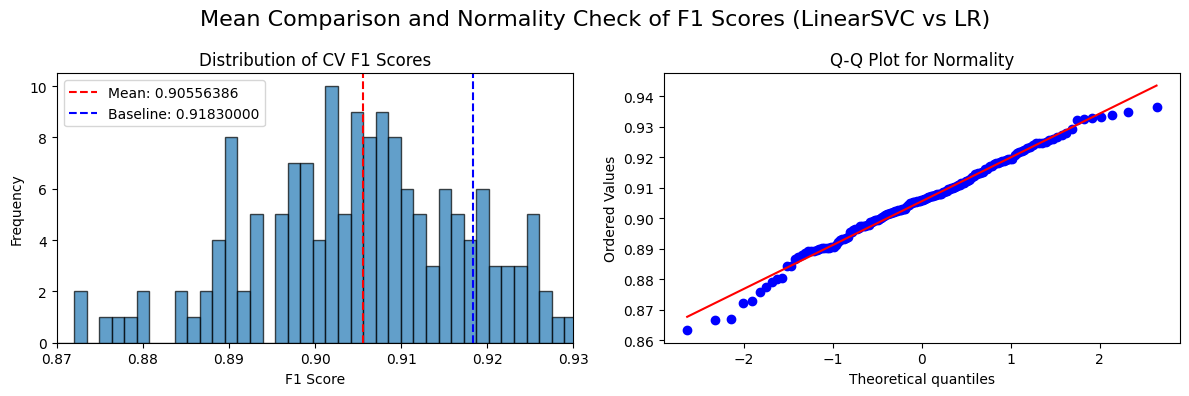
\includegraphics[keepaspectratio]{figures/30_4.9.4-svm.png}}

}

\caption{Comparing mean F1-Scores and QQ plots for LinearSVC against LR
baseline metric.}

\end{figure}%

\begin{figure}[H]

{\centering \pandocbounded{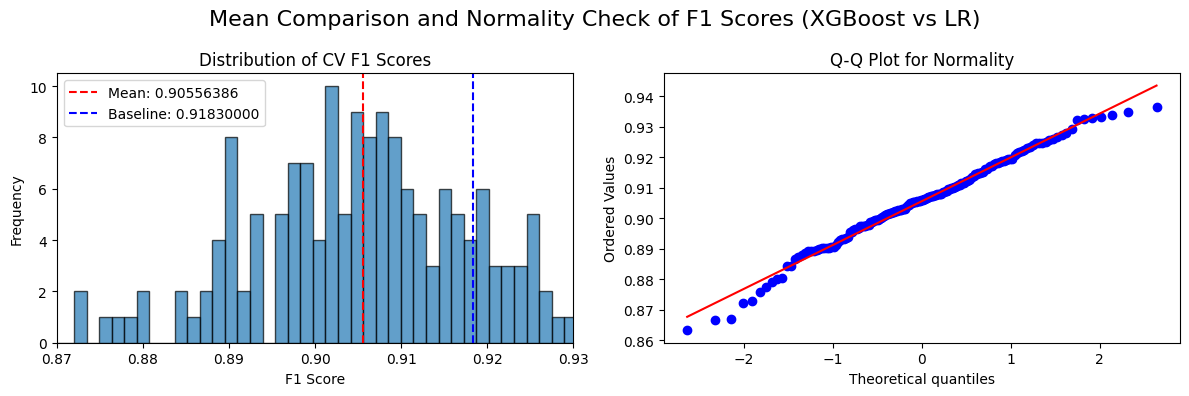
\includegraphics[keepaspectratio]{figures/30_4.9.4-xgb.png}}

}

\caption{Comparing mean F1-Scores and QQ plots for XGBoost against LR
baseline metric.}

\end{figure}%

\subsection{Statistical Significance of Dataset Size
Constraints}\label{statistical-significance-of-dataset-size-constraints}

As noted in previous sections, there are significant concerns regarding
dataset size constraints across the 13 content categories. The dataset
exhibits extreme imbalance, with certain categories containing
substantially fewer data points compared to others, ranging from 398
samples (sexedu) to 28,825 samples (alcohol) - a ratio of approximately
72:1. It is therefore of great interest whether dataset size
systematically impacts model performance across categories, exposing
potentially significant correlations that warrant careful consideration
for future data collection efforts.

The statistical correlation analysis demonstrates significant positive
relationships between dataset size and key performance metrics. Using
Spearman rank correlation to account for the extreme class imbalance and
potential non-linear relationships, the analysis revealed
medium-to-strong correlations across multiple performance dimensions.
F1-macro exhibits a significant correlation with log-transformed sample
size (\(\rho = 0.6868\), \(p = 0.009509\)), indicating that categories
with larger datasets tend to achieve substantially better F1-macro
performance. This relationship exceeds the Bonferroni-corrected
significance threshold (\(\alpha = 0.0167\)), providing strong evidence
for a systematic relationship between data availability and model
effectiveness.

\begin{figure}[H]

{\centering \pandocbounded{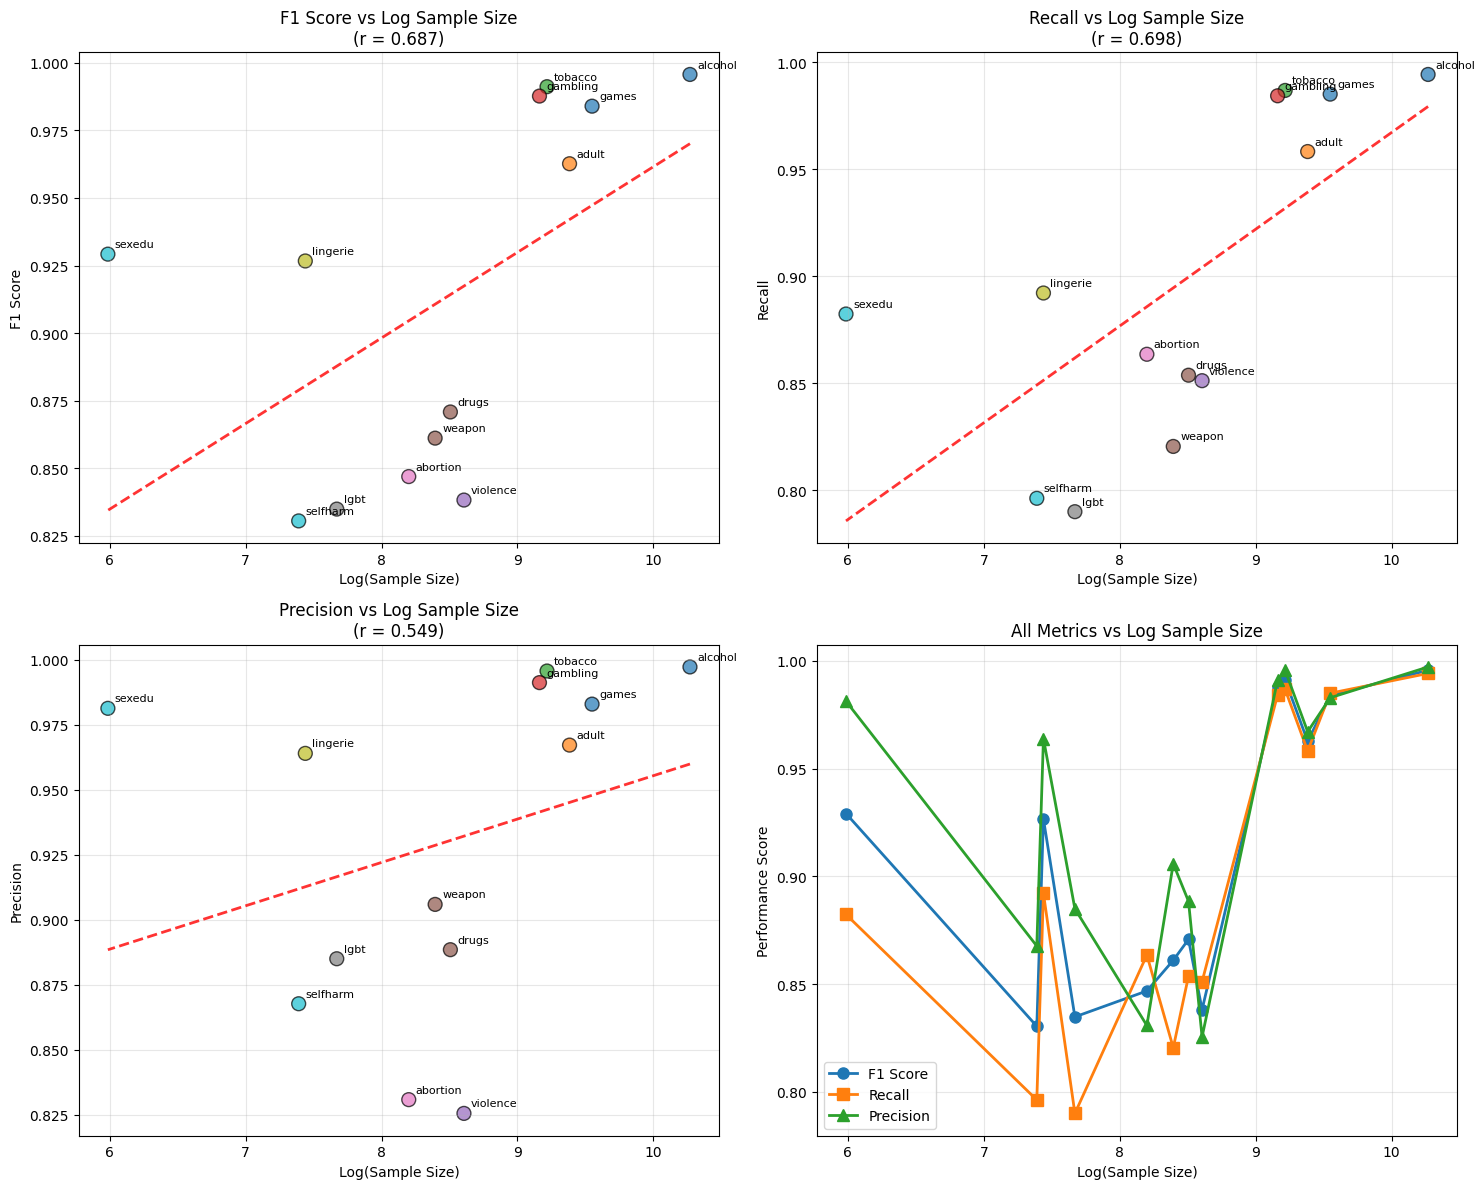
\includegraphics[keepaspectratio]{figures/31_4.9.4-3_metrics_plotted.png}}

}

\caption{F1-macro, recall, and precision fitted against log(sample
size);all metrics plotted against log(sample size)}

\end{figure}%

Similarly, recall performance demonstrates an even stronger correlation
with dataset size (\(\rho = 0.6978\), \(p = 0.008001\)), suggesting that
the model's ability to correctly identify positive instances improves
markedly with increased training examples. This finding aligns with
machine learning theory, where larger datasets typically enable better
boundary definition and reduced overfitting, particularly for minority
classes.

However, precision shows a more complex relationship (\(\rho = 0.5495\),
\(p = 0.051771\)), failing to reach statistical significance after
multiple comparison correction, indicating that the relationship between
dataset size and precision may be influenced by category-specific
characteristics beyond sample size alone.

The extreme disparity in category representation becomes evident when
examining the logarithmic distribution of sample sizes across
categories. The analysis reveals that categories with fewer than 2,000
samples (lgbt, lingerie, selfharm, sexedu) demonstrate highly variable
performance patterns, with some achieving surprisingly strong results
despite limited data. Notably, sexedu and lingerie achieve F1 scores of
0.9292 and 0.9267 respectively, suggesting that certain categories may
be inherently more discriminable or contain higher-quality features that
compensate for limited sample sizes. Dataset size by category compared
with performance metrics by category.

\begin{figure}[H]

{\centering \pandocbounded{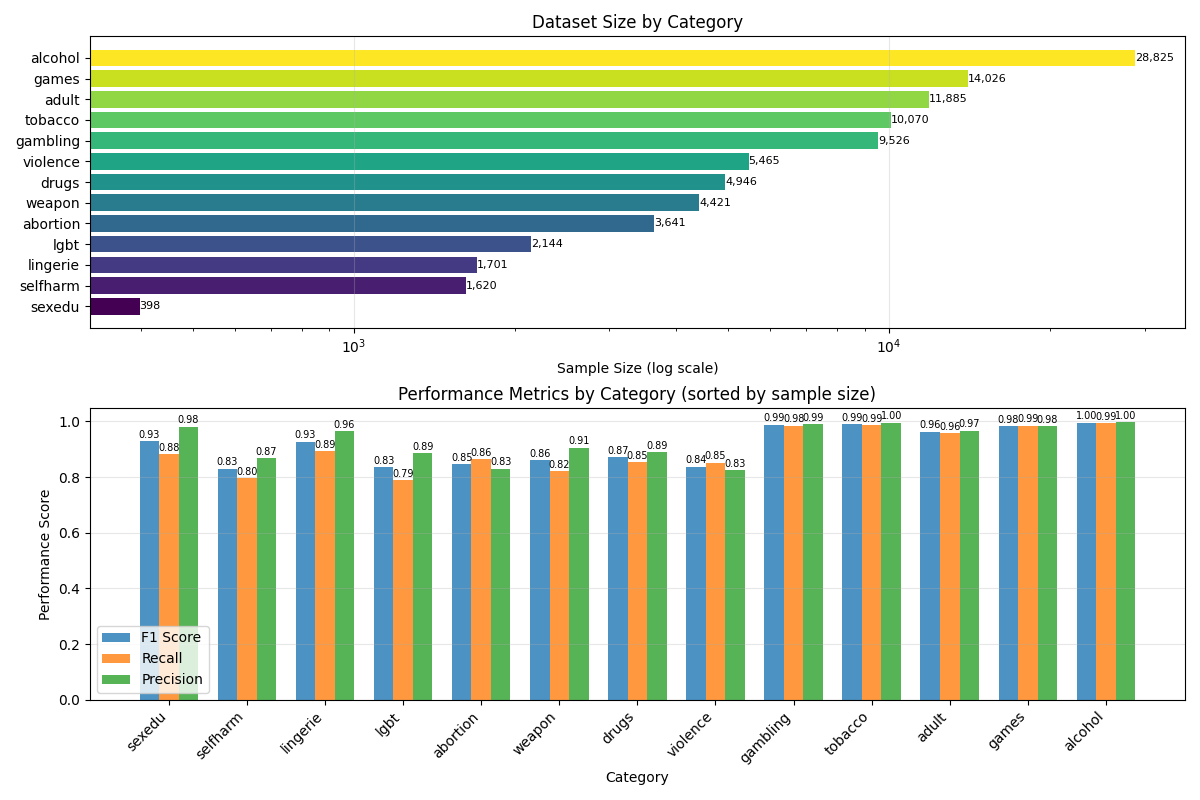
\includegraphics[keepaspectratio]{figures/32_4.9.4-dataset-size-by-category.png}}

}

\caption{Dataset size by category compared with performance metrics by
category.}

\end{figure}%

Conversely, categories with intermediate sample sizes (2,000-6,000
samples) show more consistent underperformance, particularly violence
(\(F1 = 0.8382\)), abortion (\(F1 = 0.8469\)), and selfharm
(\(F1 = 0.8305\)). This pattern suggests a complex, non-linear
relationship where moderate increases in sample size may not uniformly
translate to performance improvements, potentially due to inherent
content complexity within these specific categories.

\begin{figure}[H]

{\centering \pandocbounded{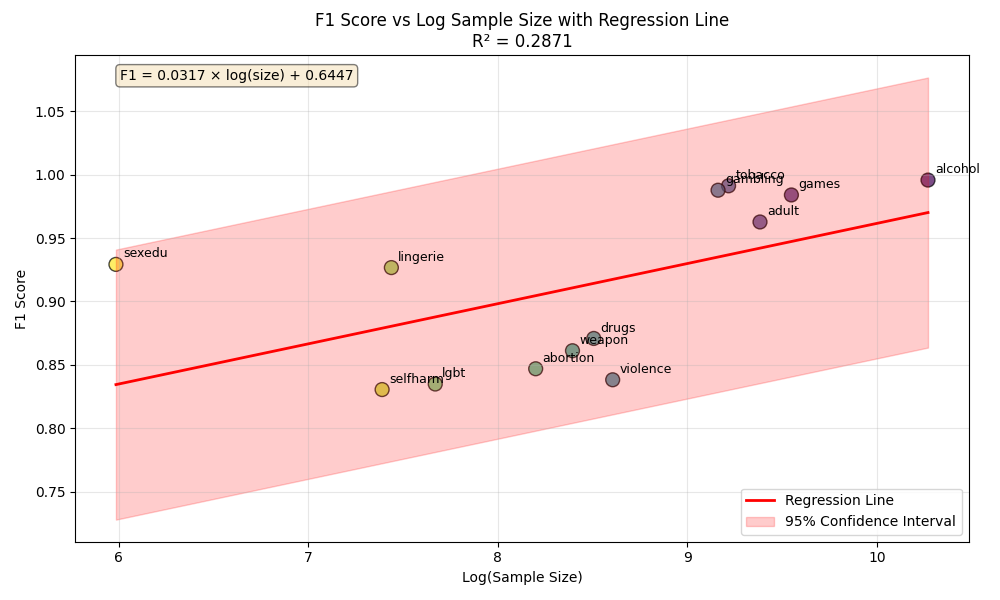
\includegraphics[keepaspectratio]{figures/33_4.9.4-f1-score-with-regression-line.png}}

}

\caption{F1-macro score vs log(sample size) against regression line with
95\% CI.}

\end{figure}%

The linear regression analysis quantifies the relationship between log
sample size and F1 performance with \(R^2 = 0.2871\), meaning that the
model explains approximately \(28.7%
\) of the variance in F1 performance through sample size alone,
indicating that while dataset size represents a meaningful predictor of
performance, other factors account for the majority of performance
variation. The positive slope coefficient (0.0317) confirms that each
unit increase in log sample size corresponds to an expected 0.0317
improvement in F1 score, providing a quantitative basis for data
collection prioritization.

The regression confidence intervals reveal substantial uncertainty
around the prediction line, particularly for categories with extreme
sample sizes. This uncertainty underscores the complexity of the
relationship and suggests that simple data augmentation may not
uniformly resolve performance disparities across all categories. The
relatively low R² value suggests that category-specific factors such as
content complexity, feature discriminability, and linguistic
characteristics play substantial roles in determining classification
performance beyond mere sample quantity.

These statistical findings provide strong empirical evidence for
prioritizing strategic data collection efforts, particularly for
underrepresented categories showing both small sample sizes and
suboptimal performance. The significant correlations (p \textless{}
0.01) for both F1 and recall metrics demonstrate that targeted data
augmentation can yield measurable performance improvements. However, the
analysis also reveals that a purely quantitative approach to data
collection may be insufficient, as evidenced by the strong performance
of some small categories and the variable relationship observed in
precision metrics.

\subsection{Implementation
Considerations}\label{implementation-considerations}

The implementation of our enhanced Chinese Web Classification Model
reveals several critical considerations that balance technical
constraints with real-world applicability. Model assumptions present
both challenges and opportunities within our specific context. While the
dataset exhibits significant multicollinearity due to the inherent
nature of overlapping content categories---such as violence and weapons,
adult content and sex education, or adult material and lingerie---our
preprocessing pipeline effectively mitigates these concerns through
strategic feature selection. The combination of TextRank and
TF-IDF-based feature extraction substantially reduces dimensionality
while preserving discriminative power, transforming a potentially
problematic characteristic into a manageable constraint. However,
logistic regression's susceptibility to overfitting, particularly given
our loss function formulation and the sparse nature of certain harmful
categories, remains a limitation that requires ongoing monitoring
through our production deployment metrics.

The practical impact of this classification system extends far beyond
technical performance metrics, directly affecting the digital safety of
hundreds of thousands of students across Taiwan's K-12 education system.
Our decision threshold analysis reflects this responsibility through
category-specific calibration: maintaining higher thresholds for
definitively inappropriate categories like games, adult content, and sex
education to ensure robust filtering, while implementing lower
thresholds for self-harm related content. This nuanced approach
acknowledges that self-harm detection serves a dual purpose, feeding
into our ActivePulse wellness monitoring system where false negatives
could have severe consequences for student wellbeing, making sensitivity
more critical than specificity in this particular domain.

From a cost-benefit perspective, the local deployment architecture of
CWCM provides significant advantages over alternative approaches. The
entirely client-side implementation eliminates ongoing API costs while
maintaining privacy and reducing latency---critical factors when
processing the browsing activities of hundreds of thousands of users
simultaneously. This approach represents substantial cost savings
compared to monolithic cloud-based solutions or LLM API calls that would
introduce prohibitive overhead and scalability challenges. While
logistic regression offers implementation simplicity comparable to
LinearSVM, it serves as our baseline model for comparison, with
production performance metrics ultimately determining the optimal
approach for our secondary detection layer development. The real-world
validation of these modeling decisions will emerge through continuous
monitoring of classification accuracy, user feedback, and administrator
responses in our deployed environment, informing the iterative
refinement necessary for maintaining effective content filtering in
Taiwan's evolving digital education landscape.

\section{Ethical Considerations}\label{ethical-considerations}

The development and deployment of automated content filtering systems in
educational environments raises significant ethical considerations
encompassing privacy implications, potential biases, cultural
sensitivity, and the balance between digital safety and access to
information. The CWCM operates primarily through client-side processing
to minimize data exposure, yet still requires access to web content for
classification tasks, representing a form of digital surveillance
managed through privacy-protective measures including zero-trust data
handling that ensures personally identifiable information is not linked
to browsing patterns. Our pursuit of ISO 27001 certification
demonstrates commitment to maintaining robust information security
standards, though technical safeguards alone are insufficient, requiring
transparency with school administrators about system operation, data
collection practices, and decision-making processes to maintain trust
and ensure informed consent (\emph{{Information security, cybersecurity
and privacy protection --- Information security management systems ---
Requirements}}, 2022).

Machine learning systems inevitably reflect biases present in their
training data and development processes, with our dataset constructed
primarily from web content identified through automated collection
methods and manual labeling processes that may introduce systematic
biases, complicated by the cultural and linguistic context of
Traditional Chinese content that may not represent the full diversity of
perspectives within Taiwan's educational community. Of particular
concern is the system's potential for differential performance across
content categories, as evidenced by our statistical analysis showing
significant performance variations correlated with dataset size, where
categories with limited training data may experience higher rates of
misclassification, potentially leading to inconsistent filtering
decisions. To mitigate these risks, we have implemented ongoing
performance monitoring across all content categories and maintain
detailed classification logs enabling retrospective analysis of system
decisions, with the client-side deployment architecture allowing for
category-specific threshold adjustments that enable educational
administrators to calibrate system sensitivity based on local context
and institutional policies.

The classification of content as ``harmful'' or ``appropriate'' is
inherently subjective and culturally dependent, with our category
definitions reflecting contemporary Taiwanese educational policy and
cultural norms that may evolve over time and may not align with all
community perspectives. We acknowledge that different educational
contexts may require different approaches to content filtering, and the
system's effectiveness depends on its alignment with local educational
objectives and community values, addressed through the modular
architecture of CWCM that allows for customization of category
definitions and classification thresholds, enabling institutions to
adapt the system to their specific needs while maintaining the
underlying technical infrastructure.

Content filtering systems face the fundamental challenge of balancing
student protection against the risk of over-censorship that could limit
educational opportunities and intellectual freedom, where overly
restrictive filtering may prevent students from accessing legitimate
educational resources, while insufficient filtering may expose students
to inappropriate content. This is addressed through several mechanisms
including the dual-layer architecture (CWCM and planned CWCM-V2)
designed to provide nuanced classification that can distinguish between
different types of content within the same domain, category-specific
threshold systems that allow for fine-tuned control over filtering
sensitivity, and most importantly, the system's design to support rather
than replace human judgment, providing administrators and educators with
tools to make informed decisions about content access.

The imperative for effective content filtering extends beyond technical
considerations to encompass well-documented public health concerns, as
extensive research demonstrates the profound impact of inappropriate
digital content exposure on student academic performance, mental health,
and cognitive development. Violence exposure in educational contexts has
been shown to significantly impair academic achievement through
disrupted school attachment and reduced motivation to succeed, while
also causing sleep disturbances that further compromise learning
outcomes (Lepore \& Kliewer, 2013; Sonsteng-Person et al., 2023). The
proliferation of digital media has introduced additional challenges,
with problematic internet use emerging as a growing concern for
adolescent health and well-being in our increasingly connected world
(Dadi et al., 2024).

Recent health advisories from major international organizations,
including the World Health Organization's warnings about teens, screens,
and mental health, and the U.S. Surgeon General's advisory on social
media and youth mental health, underscore the critical nature of these
concerns at a policy level (Office of the Surgeon General, 2023; World
Health Organization, 2024). The phenomenon of ``brain rot'' caused by
digital overload has gained recognition as a legitimate threat to
cognitive functioning, with research indicating that excessive exposure
to low-quality digital content can impair attention, memory, and
critical thinking skills essential for academic success
(\emph{Demystifying the New Dilemma of Brain Rot in the Digital Era},
2025; Lotkowski, 2025; Shanmugasundaram \& Tamilarasu, 2023). While some
studies have identified potential positive effects of certain types of
digital media under specific conditions (Egami et al., 2024), the
overwhelming consensus in the literature emphasizes the need for careful
curation of digital environments to protect developing minds from
harmful content (Heiden et al., 2019). These findings provide compelling
justification for implementing sophisticated content filtering systems
like CWCM, as the educational and psychological benefits of protecting
students from inappropriate content far outweigh the minimal privacy
considerations involved in automated classification systems designed
with robust data protection measures.

\section{Future Work}\label{future-work}

The evolution of CWCM encompasses immediate technical enhancements and
longer-term architectural improvements. Our immediate priorities focus
on deploying CWCM-V2 as a secondary detection layer using
transformer-based architectures to capture contextual information that
TF-IDF approaches miss. This dual-layer system will enable CWCM to
operate in high-recall mode while CWCM-V2 provides precision refinement
for challenging categories including self-harm, violence, and weapons.

Production evaluation will inform critical architectural decisions
through systematic comparison of Logistic Regression against LinearSVC
and XGBoost under real-world conditions. Key areas for investigation
include one-vs-rest versus multinomial classification strategies,
ensemble methods combining multiple linear models, and detailed analysis
of sigmoid versus softmax decision functions. The integration of online
learning mechanisms will enable continuous model adaptation based on
administrator feedback and emerging content patterns.

Data collection improvements address current dataset limitations through
tiered collection strategies prioritizing categories with significant
sample size-performance correlations. The training data contains
substantial noise, including non-Chinese datapoints, which requires
systematic cleaning to improve CWCM-V2 performance during fine-tuning.
Automated data collection pipelines will target underperforming
categories, while considerations for user-based data collection will
expedite the acquisition process. With CWCM-V2 deployment, CWCM
requirements shift from high F1-score performance to high recall
performance, necessitating continued experimentation with linear model
architectures for optimal integration with transformer-based attention
models.

The system's long-term development includes multilingual support
extending beyond Traditional Chinese, multimodal analysis capabilities
for harmful content in images and videos, and federated learning
frameworks enabling knowledge sharing across educational institutions
while maintaining privacy requirements. Integration with large language
models for content understanding, real-time sentiment analysis for early
intervention, and predictive modeling for proactive content curation
will transform reactive filtering into anticipatory protection. The
architecture will evolve to support personalized learning pathways
balancing content accessibility with age-appropriate safeguards while
maintaining integration with existing educational technology
infrastructure.

This development roadmap positions CWCM as an adaptive content filtering
system capable of evolving with educational needs while maintaining
effective protection of digital learning environments.

\section{Conclusion}\label{conclusion}

This study successfully developed a comprehensive enhancement to the
Chinese Web Classification Model (CWCM), addressing critical limitations
in content filtering for educational environments through systematic
data collection, rigorous algorithmic evaluation, and statistical
validation. The project constructed a substantial dataset of 429,066
Chinese web content samples with focused augmentation of harmful
categories including drugs, tobacco, and weapons, establishing a robust
foundation for machine learning-based content classification in
educational technology applications.

Our methodology evaluated over 34 machine learning algorithms through
rigorous 10-fold cross-validation, employing sophisticated preprocessing
techniques including Jieba-based text segmentation and custom TF-IDF
vectorization with strategically extracted feature dictionaries totaling
4,783 features. The optimized Logistic Regression model achieved a
macro-averaged F1-score of 0.9183, demonstrating statistically
significant superior performance compared to baseline models including
XGBoost (\(p < 0.000001\)) and LinearSVC (\(p < 0.000001\)). Statistical
correlation analysis revealed strong positive relationships between
dataset size and performance metrics (\(\rho = 0.6868\) for F1-score,
\(p = 0.009\)), providing empirical evidence for strategic data
collection priorities and informing future model development approaches.

The technical implementation successfully addresses critical deployment
constraints through client-side JavaScript architecture, enabling
real-time inference on resource-limited devices while maintaining
privacy and eliminating API dependencies. This approach represents
substantial advantages over cloud-based solutions in terms of cost,
latency, and scalability for educational institutions serving hundreds
of thousands of students. The model's multinomial classification
approach and category-specific threshold calibration demonstrate
practical considerations for balancing precision and recall across
diverse content categories, with particular attention to sensitive areas
such as self-harm detection for student wellness monitoring.

While the enhanced CWCM model represents significant theoretical and
practical improvements over existing approaches, definitive performance
validation requires extensive production deployment and AB-testing in
real educational environments. The project's comprehensive analysis of
traditional machine learning approaches---including support vector
machines, boosted trees, and linear methods---demonstrated that
statistical approaches achieve substantial classification performance
but remain limited in capturing complex semantic relationships inherent
in natural language content. This finding establishes a clear foundation
for future work incorporating transformer-based architectures in
CWCM-V2, designed to complement the current linear model through
enhanced contextual understanding.

The broader implications of this research extend beyond technical
achievement to address fundamental challenges in educational technology
deployment, digital safety, and ethical AI implementation in sensitive
environments. By providing an effective, deployable solution for Chinese
content filtering that balances accuracy, computational efficiency, and
practical implementation requirements, this work contributes
meaningfully to protecting digital learning environments while
maintaining educational accessibility and intellectual freedom. The
established methodology and findings provide a replicable framework for
content classification systems in diverse linguistic and cultural
contexts, supporting the global expansion of effective educational
technology solutions.

\section*{Appendices}\label{appendices}
\addcontentsline{toc}{section}{Appendices}

\subsection{Libraries Used}\label{libraries-used}

import os import time import random from tqdm import tqdm from selenium
import webdriver from selenium.webdriver.chrome.service import Service
from selenium.webdriver.chrome.options import Options from
selenium.webdriver.common.by import By from
selenium.webdriver.support.ui import WebDriverWait from
selenium.webdriver.support import expected\_conditions as EC from
urllib.parse import quote\_plus

from app.scrape\_logger import ScrapeLogger from app.browser import
Browser, user\_agents

import os import sys import base64 import requests from tqdm import tqdm
import concurrent.futures from bs4 import BeautifulSoup from dotenv
import load\_dotenv from urllib.parse import urlparse

from openai import OpenAI from google import genai from google.genai
import types

from error\_logger import ErrorLogger from extractor import
extract\_text, is\_valid\_website from topics import topic\_dict\_small,
topic\_dict\_medium, topic\_dict\_max

\section*{References}\label{references}
\addcontentsline{toc}{section}{References}

\phantomsection\label{refs}
\begin{CSLReferences}{1}{0}
\bibitem[\citeproctext]{ref-elith2008boosted}
A working guide to boosted regression trees. (2008). \emph{Journal of
Animal Ecology}, \emph{77}(4).
\url{https://besjournals.onlinelibrary.wiley.com/doi/10.1111/j.1365-2656.2008.01390.x}

\bibitem[\citeproctext]{ref-tensorflow2015_whitepaper}
Abadi, M., Agarwal, A., Barham, P., Brevdo, E., Chen, Z., Citro, C.,
Corrado, G. S., Davis, A., Dean, J., Devin, M., Ghemawat, S.,
Goodfellow, I., Harp, A., Irving, G., Isard, M., Jia, Y., Jozefowicz,
R., Kaiser, L., Kudlur, M., \ldots{} Zheng, X. (2016). TensorFlow:
Large-scale machine learning on heterogeneous distributed systems.
\emph{arXiv Preprint arXiv:1603.04467}.
\url{https://www.tensorflow.org/}

\bibitem[\citeproctext]{ref-bmcmedresmethodol2024calibrated}
Better calibrated probabilities in machine learning models. (2024).
\emph{BMC Medical Research Methodology}.
\url{https://bmcmedresmethodol.biomedcentral.com/articles/10.1186/s12874-024-02389-x}

\bibitem[\citeproctext]{ref-blei2003latent}
Blei, D. M., Ng, A. Y., \& Jordan, M. I. (2003). Latent dirichlet
allocation. \emph{Journal of Machine Learning Research}, \emph{3},
993--1022.

\bibitem[\citeproctext]{ref-chang2015prevention}
Chang, F.-C., Chang, Y. C., Lee, C.-M., Lung, C.-N., Liao, H.-J., Lee,
S., Miao, N.-F., Lin, S.-H., \& Zeng, W. (2015). Effects of a
school-based drug use prevention programme for middle-school students in
taiwan. \emph{Drugs: Education, Prevention and Policy}, \emph{22},
43--51. \url{https://api.semanticscholar.org/CorpusID:73334129}

\bibitem[\citeproctext]{ref-chen2016xgboost}
Chen, T., \& Guestrin, C. (2016). XGBoost: A scalable tree boosting
system. \emph{arXiv Preprint arXiv:1603.02754}.
\url{https://arxiv.org/abs/1603.02754}

\bibitem[\citeproctext]{ref-crammer2006pa}
Crammer, K., Dekel, O., Keshet, J., Shalev-Shwartz, S., \& Singer, Y.
(2006). Online passive-aggressive algorithms. \emph{Journal of Machine
Learning Research}, \emph{7}, 551--585.
\url{http://www.jmlr.org/papers/v7/crammer06a.html}

\bibitem[\citeproctext]{ref-Dadi2024}
Dadi, A. F., Dachew, B. A., \& Tessema, G. A. (2024). Problematic
internet use: A growing concern for adolescent health and well-being in
a digital era. \emph{Journal of Global Health}, \emph{14}, 03034.
\url{https://doi.org/10.7189/jogh.14.03034}

\bibitem[\citeproctext]{ref-BrainRot2025}
\emph{Demystifying the new dilemma of brain rot in the digital era}.
(2025). \url{https://pmc.ncbi.nlm.nih.gov/articles/PMC11939997/}

\bibitem[\citeproctext]{ref-scikitlearn_linearsvc}
developers, S. (n.d.). \emph{Linear models - scikit-learn
documentation}.
\url{https://scikit-learn.org/stable/modules/linear_model.html}.

\bibitem[\citeproctext]{ref-devlin2018bert}
Devlin, J., Chang, M.-W., Lee, K., \& Toutanova, K. (2018). BERT:
Pre-training of deep bidirectional transformers for language
understanding. \emph{arXiv Preprint arXiv:1810.04805}.
\url{https://arxiv.org/abs/1810.04805}

\bibitem[\citeproctext]{ref-frontiers2025digital}
Digital education research trends 2014-2023. (2025). \emph{Frontiers in
Education}.
\url{https://www.frontiersin.org/journals/education/articles/10.3389/feduc.2025.1533588/full}

\bibitem[\citeproctext]{ref-Egami2024}
Egami, H., Rahman, Md. S., Yamamoto, T., Egami, C., \& Wakabayashi, T.
(2024). Causal effect of video gaming on mental well-being in japan
2020--2022. \emph{Nature Human Behaviour}, \emph{8}(10), 1943--1956.
\url{https://doi.org/10.1038/s41562-024-01948-y}

\bibitem[\citeproctext]{ref-kibana}
Elastic. (2025). \emph{Kibana: Data visualization and exploration}.
\url{https://www.elastic.co/kibana}.

\bibitem[\citeproctext]{ref-fan2008liblinear}
Fan, R.-E., Chang, K.-W., Hsieh, C.-J., Wang, X.-R., \& Lin, C.-J.
(2008). LIBLINEAR: A library for large linear classification.
\emph{Journal of Machine Learning Research}, \emph{9}, 1871--1874.

\bibitem[\citeproctext]{ref-stanford2023finetuning}
\emph{Fine-tuning strategies for task adaptation}. (2023). Stanford
University.
\url{https://web.stanford.edu/class/archive/cs/cs224n/cs224n.1234/final-reports/final-report-169710070.pdf}

\bibitem[\citeproctext]{ref-jieba}
fxsjy. (n.d.). \emph{{jieba: Chinese text segmentation}} (Version refer
to GitHub for current release) {[}Computer software{]}.
\url{https://github.com/fxsjy/jieba}

\bibitem[\citeproctext]{ref-geeksforgeeks2025hinge}
GeeksforGeeks. (2025). \emph{Hinge-loss \& relationship with support
vector machines}. GeeksforGeeks;
\url{https://www.geeksforgeeks.org/hinge-loss-relationship-with-support-vector-machines/}.

\bibitem[\citeproctext]{ref-vonDerHeiden2019}
Heiden, J. M. von der, Braun, B., Müller, K. W., \& Egloff, B. (2019).
The association between video gaming and psychological functioning.
\emph{Frontiers in Psychology}, \emph{10}, 1731.
\url{https://doi.org/10.3389/fpsyg.2019.01731}

\bibitem[\citeproctext]{ref-hochreiter1997lstm}
Hochreiter, S., \& Schmidhuber, J. (1997). Long short-term memory.
\emph{Neural Computation}.
\url{https://www.bioinf.jku.at/publications/older/2604.pdf}

\bibitem[\citeproctext]{ref-holoniq2025}
HolonIQ. (2025). \emph{Global education technology market to reach
\$404B by 2025}.
\url{https://www.holoniq.com/notes/global-education-technology-market-to-reach-404b-by-2025}

\bibitem[\citeproctext]{ref-ISO27001}
\emph{{Information security, cybersecurity and privacy protection ---
Information security management systems --- Requirements}} (Vol. 3).
(2022). (Vol. 3) {[}Standard{]}. International Organization for
Standardization.

\bibitem[\citeproctext]{ref-jare2023defendnet}
Jare, A., \& Kolte, S. (2023). DefendNet: Harnessing AI/ML for dynamic
DNS and web filtering. \emph{Semantic Scholar}.
\url{https://www.semanticscholar.org/paper/DefendNet\%3A-Harnessing-AI-ML-for-Dynamic-DNS-and-Jare-Kolte/d2b8abf7ff9a85d7d58e85ca319bdc902a92497f}

\bibitem[\citeproctext]{ref-jolliffe2002principal}
Jolliffe, I. T. (2002). \emph{Principal component analysis} (2nd ed.).
Springer.

\bibitem[\citeproctext]{ref-osti_6910294}
Jordan, M. I. (1986). \emph{Serial order: A parallel distributed
processing approach. Technical report, june 1985-march 1986}. California
Univ., San Diego, La Jolla (USA). Inst. for Cognitive Science.
\url{https://www.osti.gov/biblio/6910294}

\bibitem[\citeproctext]{ref-junco2014media}
Junco, R. (2014). Media multitasking and academic performance.
\emph{Computers \& Education}.
\url{https://www.sciencedirect.com/science/article/abs/pii/S0360131514001158}

\bibitem[\citeproctext]{ref-lee2013l2multiclass}
Lee, C.-P., \& Lin, C.-J. (2013). A study on L2-loss (squared
hinge-loss) multiclass SVM. \emph{Neural Computation}, \emph{25}(5),
1302--1323. \url{https://doi.org/10.1162/NECO/_a/_00434}

\bibitem[\citeproctext]{ref-Lepore2013}
Lepore, S. J., \& Kliewer, W. (2013). Violence exposure, sleep
disturbance, and poor academic performance in middle school.
\emph{Journal of Abnormal Child Psychology}, \emph{41}(8), 1179--1189.
\url{https://doi.org/10.1007/s10802-013-9709-0}

\bibitem[\citeproctext]{ref-Levine2012}
Levine, L. E., Waite, B. M., \& Bowman, L. L. (2012). Mobile media use,
multitasking and distractibility. \emph{International Journal of Cyber
Behavior, Psychology and Learning}, \emph{2}(3), 15--29.
\url{https://doi.org/10.4018/ijcbpl.2012070102}

\bibitem[\citeproctext]{ref-ke2017lightgbm}
LightGBM: A highly efficient gradient boosting decision tree. (2017).
\emph{Advances in Neural Information Processing Systems}.
\url{https://proceedings.neurips.cc/paper_files/paper/2017/file/6449f44a102fde848669bdd9eb6b76fa-Paper.pdf}

\bibitem[\citeproctext]{ref-lin2021healthliteracy}
Lin, L. C., Huang, C. M., Hsu, H. P., Liao, J. Y., Lin, C. Y., \& Guo,
J. L. (2021). Integrating health literacy into a theory-based drug-use
prevention program: A quasi-experimental study among junior high
students in taiwan. \emph{BMC Public Health}, \emph{21}(1), 1768.
\url{https://doi.org/10.1186/s12889-021-11830-5}

\bibitem[\citeproctext]{ref-liu2019roberta}
Liu, Y., Ott, M., Goyal, N., Du, J., Joshi, M., Chen, D., Levy, O.,
Lewis, M., Zettlemoyer, L., \& Stoyanov, V. (2019). RoBERTa: A robustly
optimized BERT pretraining approach. \emph{arXiv Preprint
arXiv:1907.11692}. \url{https://arxiv.org/abs/1907.11692}

\bibitem[\citeproctext]{ref-InspiraHealth2025}
Lotkowski, S. (2025). \emph{Brain rot explained: How digital overload
affects your mind}. Inspira Health Network.
\url{https://www.inspirahealthnetwork.org/news/healthy-living/brain-rot-explained-how-digital-overload-affects-your-mind}

\bibitem[\citeproctext]{ref-mihalcea2004textrank}
Mihalcea, R., \& Tarau, P. (2004). TextRank: Bringing order into text.
\emph{Proceedings of the 2004 Conference on Empirical Methods in Natural
Language Processing}, 404--411.

\bibitem[\citeproctext]{ref-steep_drop_performance}
Mutsam, N., Fuchs, A., Ziegler, F., \& Pernkopf, F. (2024). Data-scarce
condition modeling requires model-based prior regularization.
\emph{ICASSP 2024 - 2024 IEEE International Conference on Acoustics,
Speech and Signal Processing (ICASSP)}, 6695--6699.
\url{https://doi.org/10.1109/ICASSP48485.2024.10446987}

\bibitem[\citeproctext]{ref-oecd2023pisa}
OECD. (2023). \emph{PISA 2022 assessment and analytical framework}.
Organisation for Economic Co-operation; Development.
\url{https://www.oecd.org/content/dam/oecd/en/publications/reports/2023/08/pisa-2022-assessment-and-analytical-framework_a124aec8/dfe0bf9c-en.pdf}

\bibitem[\citeproctext]{ref-oecd2024screen}
OECD. (2024). \emph{Managing screen time: PISA 2022 results}.
Organisation for Economic Co-operation; Development.
\url{https://www.oecd.org/content/dam/oecd/en/publications/reports/2024/05/managing-screen-time_023f2390/7c225af4-en.pdf}

\bibitem[\citeproctext]{ref-SurgeonGeneral2023}
Office of the Surgeon General. (2023). \emph{Social media and youth
mental health: The u.s. Surgeon general's advisory}. U.S. Department of
Health; Human Services.
\url{https://www.hhs.gov/surgeongeneral/reports-and-publications/youth-mental-health/social-media/index.html}

\bibitem[\citeproctext]{ref-peters2018elmo}
Peters, M. E., Neumann, M., Iyyer, M., Gardner, M., Clark, C., Lee, K.,
\& Zettlemoyer, L. (2018). Deep contextualized word representations.
\emph{Proceedings of the 2018 Conference of the North American Chapter
of the Association for Computational Linguistics: Human Language
Technologies}. \url{https://aclanthology.org/N18-1202.pdf}

\bibitem[\citeproctext]{ref-press2021alibi}
Press, O., Smith, N. A., \& Lewis, M. (2021). Train short, test long:
Attention with linear biases enables input length extrapolation.
\emph{arXiv Preprint arXiv:2108.12409}.
\url{https://arxiv.org/abs/2108.12409}

\bibitem[\citeproctext]{ref-qureshi2023digital}
Qureshi, M. I., \& Khan, N. (2023). Digital technologies in education
4.0. Does it enhance the learning experience? \emph{Semantic Scholar}.
\url{https://www.semanticscholar.org/paper/Digital-Technologies-in-Education-4.0.-Does-it-the-Qureshi-Khan/ba699042e175b7aa3d48a49787131b3a2b7a7dd0}

\bibitem[\citeproctext]{ref-radford2018gpt}
Radford, A., Narasimhan, K., Salimans, T., \& Sutskever, I. (2018).
\emph{Improving language understanding by generative pre-training}.
OpenAI.
\url{https://cdn.openai.com/research-covers/language-unsupervised/language_understanding_paper.pdf}

\bibitem[\citeproctext]{ref-RAGAN201478}
Ragan, E. D., Jennings, S. R., Massey, J. D., \& Doolittle, P. E.
(2014). Unregulated use of laptops over time in large lecture classes.
\emph{Computers \& Education}, \emph{78}, 78--86.
https://doi.org/\url{https://doi.org/10.1016/j.compedu.2014.05.002}

\bibitem[\citeproctext]{ref-sanh2019distilbert}
Sanh, V., Debut, L., Chaumond, J., \& Wolf, T. (2019). DistilBERT, a
distilled version of BERT: Smaller, faster, cheaper and lighter.
\emph{arXiv Preprint arXiv:1910.01108}.
\url{https://arxiv.org/pdf/1910.01108}

\bibitem[\citeproctext]{ref-schmidt2019recurrent}
Schmidt, R. M. (2019). Recurrent neural networks (RNNs): A gentle
introduction and overview. \emph{arXiv Preprint arXiv:1912.05911}.
\url{https://arxiv.org/abs/1912.05911}

\bibitem[\citeproctext]{ref-seal2006preventing}
Seal, N. (2006). Preventing tobacco and drug use among thai high school
students through life skills training. \emph{Nursing \& Health
Sciences}, \emph{8 3}, 164--168.
\url{https://api.semanticscholar.org/CorpusID:7553748}

\bibitem[\citeproctext]{ref-Shanmugasundaram2023}
Shanmugasundaram, M., \& Tamilarasu, A. (2023). The impact of digital
technology, social media, and artificial intelligence on cognitive
functions: A review. \emph{Frontiers in Cognition}, \emph{2}, 1203077.
\url{https://doi.org/10.3389/fcogn.2023.1203077}

\bibitem[\citeproctext]{ref-Sharma2014SeleniumTA}
Sharma, M. (2014). \emph{Selenium tool: A web based automation testing
framework}. \url{https://api.semanticscholar.org/CorpusID:18049611}

\bibitem[\citeproctext]{ref-smith2024bert_architecture_diagram}
Smith, B. (2024). \emph{A comparison of the architectures for the
transformer, GPT, and BERT}. A Complete Guide to BERT with Code, Towards
Data Science.
\url{https://towardsdatascience.com/a-complete-guide-to-bert-with-code-9f87602e4a11/}

\bibitem[\citeproctext]{ref-SonstengPerson2023}
Sonsteng-Person, M., Jaggers, J. W., \& Loomis, A. M. (2023). Academic
achievement after violence exposure: The indirect effects of school
attachment and motivation to succeed. \emph{Journal of Child and
Adolescent Trauma}, \emph{16}(3), 717--729.
\url{https://doi.org/10.1007/s40653-023-00546-w}

\bibitem[\citeproctext]{ref-iza2018students}
\emph{Student device usage patterns} (11455). (2018). Institute for
Labor Economics. \url{https://docs.iza.org/dp11455.pdf}

\bibitem[\citeproctext]{ref-sturua2023jinabert}
Sturua, S., Wang, N., Kosson, A., \& Xiao, H. (2023). JinaBERT:
Extending BERT for long documents with ALiBi. \emph{arXiv Preprint
arXiv:2310.19923}. \url{https://arxiv.org/pdf/2310.19923}

\bibitem[\citeproctext]{ref-chen2021taiwan}
Substance use among adolescents in taiwan: A systematic review. (2021).
\emph{PMC}. \url{https://pmc.ncbi.nlm.nih.gov/articles/PMC8479915/}

\bibitem[\citeproctext]{ref-svm2018ideal}
Support vector machines as ideal candidates for sparse data
classification. (2018). \emph{Artificial Intelligence in Medicine}.
\url{https://www.sciencedirect.com/science/article/abs/pii/S0933365718303294?via=ihub}

\bibitem[\citeproctext]{ref-dimensionality2017}
Support vector machines performance in high dimensional data. (2017).
\emph{European Journal of Operational Research}.
\url{https://linkinghub.elsevier.com/retrieve/pii/S0377221717307713}

\bibitem[\citeproctext]{ref-cognitive2013task}
Task switching and cognitive performance. (2013). \emph{PsycNet APA}.
\url{https://psycnet.apa.org/record/2013-03177-002}

\bibitem[\citeproctext]{ref-tripathi2021rnn_lstm_diagram}
Tripathi, A. (2021). \emph{RNN unit vs LSTM unit architecture
comparison}. What is the main difference between RNN and LSTM \textbar{}
NLP \textbar{} RNN vs LSTM, Data Science Duniya.
\url{https://ashutoshtripathi.com/2021/07/02/what-is-the-main-difference-between-rnn-and-lstm-nlp-rnn-vs-lstm/}

\bibitem[\citeproctext]{ref-unesco2023gem}
UNESCO. (2023). \emph{Global education monitoring report 2023:
Technology in education: A tool on whose terms?} UNESCO.
\url{https://www.unesco.org/gem-report/sites/default/files/medias/fichiers/2023/07/Summary_v5.pdf}

\bibitem[\citeproctext]{ref-maaten2008visualizing}
Van der Maaten, L., \& Hinton, G. (2008). Visualizing data using t-SNE.
\emph{Journal of Machine Learning Research}, \emph{9}(11), 2579--2605.

\bibitem[\citeproctext]{ref-vaswani2017attention}
Vaswani, A., Shazeer, N., Parmar, N., Uszkoreit, J., Jones, L., Gomez,
A. N., Kaiser, Ł., \& Polosukhin, I. (2017). Attention is all you need.
\emph{arXiv Preprint arXiv:1706.03762}.
\url{https://arxiv.org/abs/1706.03762}

\bibitem[\citeproctext]{ref-wang2018glue}
Wang, A., Singh, A., Michael, J., Hill, F., Levy, O., \& Bowman, S. R.
(2018). GLUE: A multi-task benchmark and analysis platform for natural
language understanding. \emph{International Conference on Learning
Representations}. \url{https://openreview.net/pdf?id=rJ4km2R5t7}

\bibitem[\citeproctext]{ref-Ward2017}
Ward, A. F., Duke, K., Gneezy, A., \& Bos, M. W. (2017). Brain drain:
The mere presence of one's own smartphone reduces available cognitive
capacity. \emph{Journal of the Association for Consumer Research},
\emph{2}(2), 140--154. \url{https://doi.org/10.1086/691462}

\bibitem[\citeproctext]{ref-wen2018efficient}
Wen, Z. (2018). Efficient computing algorithm for high dimensional
support vector machines. \emph{Semantic Scholar}.
\url{https://www.semanticscholar.org/paper/Efficient-Computing-Algorithm-for-High-Dimensional-Wen/67982784a395129e0683d973d2cd1ddaea30a6ef}

\bibitem[\citeproctext]{ref-WHO2024}
World Health Organization. (2024). \emph{Teens, screens and mental
health}.
\url{https://www.who.int/europe/news/item/25-09-2024-teens--screens-and-mental-health}

\bibitem[\citeproctext]{ref-nodejieba}
Wu, Y., \& contributors. (2025). \emph{NodeJieba: Node.js chinese word
segmentation}. \url{https://github.com/yanyiwu/nodejieba}.

\end{CSLReferences}




\end{document}
